%\pdfoutput=1
% Uncomment line above if submitting to arXiv and using pdflatex

% $Id: main.tex 97873 2016-09-08 18:28:41Z michaelt $
% ============================================================================
% Purpose: Template for LHCb documents
% Authors: Tomasz Skwarnicki, Roger Forty, Ulrik Egede
% Created on: 2010-09-24
% ============================================================================
\documentclass[12pt,a4paper]{article}
%%\documentclass[12pt,letter]{article}
% For two column text, add "twocolumn" as an option to the document
% class. Also uncomment the two "onecolumn" and "twocolumn" lines
% around the title page below.

% Variables that controls behaviour
\usepackage{ifthen} % for conditional statements
\newboolean{pdflatex}
\setboolean{pdflatex}{true} % False for eps figures 

\newboolean{articletitles}
\setboolean{articletitles}{true} % False removes titles in references

\newboolean{uprightparticles}
\setboolean{uprightparticles}{false} %True for upright particle symbols

\newboolean{inbibliography}
\setboolean{inbibliography}{false} %True once you enter the bibliography


\newcommand{\phs}{\ensuremath{\Phi_4}}  %% phase space
\newcommand{\phsd}{\ensuremath{\phi_4}} %% phase space density
\newcommand{\dphs}{\ensuremath{\mathrm{d}\phs}}  

\newcommand{\phsPoint}{\ensuremath{\mathbf{x}}}
\newcommand{\dphsPoint}{\ensuremath{\mathrm{d}^5x}}
\newcommand{\phsPointCP}{\ensuremath{\overline{\mathbf{x}}}}
\newcommand{\dphsPointCP}{\ensuremath{\mathrm{d}^5\overline{x}}}

\newcommand{\cleoc}{{C}{L}{E}{O}{-}{c}}

\newcommand{\prt}[1]{\ensuremath{#1}} %% for particle names
\newcommand{\DDbar}{\prt{D\overline{D}}}
\newcommand{\fourpi}{\prt{\pi^+\pi^-\pi^+\pi^-}}
\newcommand{\KKpipi}{\prt{K^+K^-\pi^+\pi^-}}

\newcommand{\eqnref}[1]{Eq.~\ref{#1}}
\newcommand{\eqnPRDref}[1]{Eq.~(\ref{#1})}
\newcommand{\Eqnref}[1]{Equation~\ref{#1}}
\newcommand{\EqnPRDref}[1]{Equation~(\ref{#1})}
\newcommand{\figref}[1]{Fig.~\ref{#1}}
\newcommand{\Figref}[1]{Figure~\ref{#1}}
\newcommand{\tabref}[1]{Tab.~\ref{#1}}
\newcommand{\Tabref}[1]{Table~\ref{#1}}
\newcommand{\secref}[1]{Sec.~\ref{#1}}
\newcommand{\Secref}[1]{Section~\ref{#1}}
\newcommand{\appref}[1]{App.~\ref{#1}}
\newcommand{\Appref}[1]{Appendix~\ref{#1}}

%%

\input{preamble}

\usepackage{pifont}
\definecolor{darkgreen}{rgb}{0.0,0.5,0.0}
\definecolor{darkred}{rgb}{0.5,0.0,0.0}

\renewcommand{\thefigure}{\arabic{section}.\arabic{figure}}
\makeatletter \@addtoreset{figure}{section} \makeatother

\renewcommand{\theequation}{\arabic{section}.\arabic{equation}}
\makeatletter \@addtoreset{equation}{section} \makeatother

\renewcommand{\thetable}{\arabic{section}.\arabic{table}}
\makeatletter \@addtoreset{table}{section} \makeatother

\usepackage{longtable} % only for template; not usually to be used in PAPERs
\usepackage[labelfont=bf]{caption}

%\usepackage{tikz}
%  \usetikzlibrary{shapes}
%  \usetikzlibrary{patterns,circuits.ee.IEC}
%\usepackage{tkz-euclide}
%\usetkzobj{all}

%\usetikzlibrary{external}
%\tikzexternalize
%\tikzexternalize[prefix=./]

\usepackage{booktabs}
\usepackage[nottoc]{tocbibind}
\usepackage{cite}
\usepackage{subcaption}

\usepackage{multirow}
\usepackage{rotating}

\usepackage[draft, textwidth=1.75cm]{todonotes} % added by PN on 24 Feb 2017 to better deal with tracking comments within the paper
%\usepackage[disable]{todonotes} % this hides all comments when TeXing the paper
\newcommand{\comment}[1]{\todo[color=blue!40, size=\tiny, fancyline]{#1}}
\newcommand{\pretextcomment}[1]{\todo[color=blue!40, inline, nolist]{#1}}
\setlength{\marginparwidth}{2.25cm} % currently needed to get todos to look right
\reversemarginpar 
\begin{document}

%%%%%%%%%%%%%%%%%%%%%%%%%
%%%%% Title     %%%%%%%%%
%%%%%%%%%%%%%%%%%%%%%%%%%
\renewcommand{\thefootnote}{\fnsymbol{footnote}}
\setcounter{footnote}{1}

% %%%%%%% CHOOSE TITLE PAGE--------
%\onecolumn
%\input{title-LHCb-INT}
% $Id: title-LHCb-ANA.tex 39841 2013-07-26 10:31:08Z roldeman $
% ===============================================================================
% Purpose: LHCb-ANA Note title page template
% Author: 
% Created on: 2010-10-05
% ===============================================================================

%%%%%%%%%%%%%%%%%%%%%%%%%
%%%%%  TITLE PAGE  %%%%%%
%%%%%%%%%%%%%%%%%%%%%%%%%
\begin{titlepage}

% Header ---------------------------------------------------
\vspace*{-1.5cm}

\noindent
\begin{tabular*}{\linewidth}{lc@{\extracolsep{\fill}}r@{\extracolsep{0pt}}}
\ifthenelse{\boolean{pdflatex}}% Logo format choice
{\vspace*{-2.7cm}\mbox{\!\!\!\includegraphics[width=.14\textwidth]{lhcb-logo.pdf}} & &}%
{\vspace*{-1.2cm}\mbox{\!\!\!\includegraphics[width=.12\textwidth]{lhcb-logo.eps}} & &}
 \\
 & & LHCb-ANA-2018-021 \\  % ID 
 & & \today \\ % Date - Can also hardwire e.g.: 23 March 2010
 & & v3.1 \\
\hline
\end{tabular*}

\vspace*{4.0cm}

% Title --------------------------------------------------
{\normalfont\bfseries\boldmath\huge
\begin{center}
Measurement of the CKM angle $\gamma$ using $\Bs\to\Ds\kaon\pion\pion$ decays
\end{center}
}

\vspace*{2.0cm}

% Authors -------------------------------------------------
\begin{center}
P. d'Argent$^1$, E. Gersabeck$^2$, M. Kecke$^1$, M. Schiller$^3$
\bigskip\\
{\normalfont\itshape\footnotesize
$ ^1$Physikalisches Institut, Ruprecht-Karls-Universit\"at Heidelberg, Heidelberg, Germany\\
$ ^2$School of Physics and Astronomy, University of Manchester, Manchester, United Kingdom\\
$ ^3$School of Physics and Astronomy, University of Glasgow, Glasgow, United Kingdom\\
}
\end{center}

\vspace{\fill}

% Abstract -----------------------------------------------
\begin{abstract}
  \noindent
We present the first measurement of the weak phase $\gamma-2\beta_s$ obtained from a time-dependent (amplitude) analysis of 
$\Bs \to \Ds K \pi \pi$ decays using 
proton-proton collision data corresponding to an integrated luminosity of  $7 \invfb$ recorded by the LHCb detector.

\end{abstract}

\vspace*{2.0cm}
\vspace{\fill}

\end{titlepage}


\pagestyle{empty}  % no page number for the title 

%%%%%%%%%%%%%%%%%%%%%%%%%%%%%%%%
%%%%%  EOD OF TITLE PAGE  %%%%%%
%%%%%%%%%%%%%%%%%%%%%%%%%%%%%%%%

%  empty page follows the title page ----
\newpage
\setcounter{page}{2}
\mbox{~}

\cleardoublepage

%\input{title-LHCb-CONF}
%% $Id: title-LHCb-PAPER.tex 122889 2018-08-17 17:59:55Z pkoppenb $
% ===============================================================================
% Purpose: LHCb-PAPER journal paper title page template
% Author: 
% Created on: 2010-09-25
% ===============================================================================

%%%%%%%%%%%%%%%%%%%%%%%%%
%%%%%  TITLE PAGE  %%%%%%
%%%%%%%%%%%%%%%%%%%%%%%%%
\begin{titlepage}
\pagenumbering{roman}

% Header ---------------------------------------------------
\vspace*{-1.5cm}
\centerline{\large EUROPEAN ORGANIZATION FOR NUCLEAR RESEARCH (CERN)}
\vspace*{1.5cm}
\noindent
\begin{tabular*}{\linewidth}{lc@{\extracolsep{\fill}}r@{\extracolsep{0pt}}}
\ifthenelse{\boolean{pdflatex}}% Logo format choice
{\vspace*{-1.5cm}\mbox{\!\!\!\includegraphics[width=.14\textwidth]{figs/lhcb-logo.pdf}} & &}%
{\vspace*{-1.2cm}\mbox{\!\!\!\includegraphics[width=.12\textwidth]{figs/lhcb-logo.eps}} & &}%
\\
 & & CERN-EP-20XX-ZZZ \\  % ID 
 & & LHCb-PAPER-20XX-YYY \\  % ID 
 & & \today \\ % Date - Can also hardwire e.g.: 23 March 2010
 & & \\
% not in paper \hline
\end{tabular*}

\vspace*{1.5cm}

% Title --------------------------------------------------
{\normalfont\bfseries\boldmath\huge
\begin{center}
% DO NOT EDIT HERE. Instead edit macro in main.tex to keep metadata correct
  \papertitle 
\end{center}
}

%\vspace*{2.0cm}

% Authors -------------------------------------------------
\begin{center}
%In the footnote, replace 'paper' by 'Letter' in case of submission to PRL or PLB 
% Edit macro in main.tex to keep metadata correct
\paperauthors\footnote{Authors are listed at the end of this paper.}
\end{center}

\vspace{\fill}

% Abstract -----------------------------------------------
\begin{abstract}
  \noindent \small
The measurement of the CKM angle $\gamma$, as well as the \CP-violating parameters in $\Bs\to\Dspm\Kpm\pion\pion$ decays, is reported.
For the measurement, a data set of $pp$ collisions, corresponding to an integrated luminosity of 7 $\invfb$, recorded with the \lhcb detector, is used.
The CP-violating parameters are measured to be $C_{f} = y \pm Y \pm y$, $A^{\DG}_{f} = x \pm X \pm x$, $A^{\DG}_{\bar{f}} = x \pm Y \pm x$, $S_{f} = x \pm X \pm x$ and $S_{\bar{f}} = x \pm Y \pm x$, 
where the uncertainties are statistical and systematic, respectively. 
These parameters are used in combination with the world-average of the weak $\Bs$ mixing phase $\beta_{s}$, to obtain a model-independent meaurement of the CKM angle $\gamma$.
The measurement yields $\gamma = (2000^{+x}_{-a})\degrees$ modulo $180\degrees$, where the uncertainty contains both statistical and systematic errors.
A model-dependent measurement, using an amplitude model to describe the non-trivial phase-space of this decay, yields $\gamma = (1934^{+x}_{-a})\degrees$.
Using a sample of $\Bs\to\Ds\pion\pion\pion$ decays, found in the same \lhcb data set, the $\Bs$ oscillation fequency is measured to be $\dms = xx.xx \pm yy.yy \pm zz.zz$, 
where the uncertainties are statistical and systematic, respectively. \normalsize
\end{abstract}

\vspace*{2.0cm}

\begin{center}
  Submitted to JHEP / Phys.~Rev.~D / Phys.~Rev.~Lett. / Phys.~Lett.~B / Eur.~Phys.~J.~C / Nucl.~Phys.~B 
\end{center}

\vspace{\fill}

{\footnotesize 
% Edit macro in main.tex to keep metadata correct
\centerline{\copyright~\papercopyright. \href{\paperlicenceurl}{\paperlicence}.}}
\vspace*{2mm}

\end{titlepage}


%%%%%%%%%%%%%%%%%%%%%%%%%%%%%%%%
%%%%%  EOD OF TITLE PAGE  %%%%%%
%%%%%%%%%%%%%%%%%%%%%%%%%%%%%%%%

%  empty page follows the title page ----
\newpage
\setcounter{page}{2}
\mbox{~}
%\newpage
%
%% Author List ----------------------------
%%  You need to get a new author list!
%\input{LHCb_authorlist.tex}
%
%The author list for journal publications is provided by the Membership Committee shortly after 'approval to go to paper' has been given.
%%It will be made available on the page
%%\verb!http://www.physik.uzh.ch/~strauman/forMemCo/LHCb-PAPER-XXXX-XXX/! .
%It will be sent to you by email shortly after a paper number has beens assigned.
%The author list should be included already at first circulation, 
%to allow new members of the collaboration to verify whether they have been included correctly.
%Occasionally a misspelled name is corrected or associated institutions become full members.
%In that case, a new author list will be sent to you.
%In case line numbering doesn't work well after including the authorlist, try moving the \verb!\bigskip! after the last author to a separate line.
%
%
%The authorship for Conference Reports should be ``The LHCb
%  collaboration'', with a footnote giving the name(s) of the contact
%  author(s), but without the full list of collaboration names.



\cleardoublepage








%\twocolumn
% %%%%%%%%%%%%% ---------

\renewcommand{\thefootnote}{\arabic{footnote}}
\setcounter{footnote}{0}


\pagenumbering{gobble}
%%%%%%%%%%%%%%%%%%%%%%%%%%%%%%%%
%%%%%  Table of Content   %%%%%%
%%%%%%%%%%%%%%%%%%%%%%%%%%%%%%%%
%%%% Uncomment next 2 lines if desired
\tableofcontents
\cleardoublepage


%%%%%%%%%%%%%%%%%%%%%%%%%
%%%%% Main text %%%%%%%%%
%%%%%%%%%%%%%%%%%%%%%%%%%

\pagestyle{plain} % restore page numbers for the main text
\setcounter{page}{1}
\pagenumbering{arabic}

%% Uncomment during review phase. 
%% Comment before a final submission.
\linenumbers

%% !TEX root = main.tex

\setcounter{section}{-1}
\section{To do list}

\begin{enumerate}
	\item Efficiencies for 2012. Need MC12 for normalization channel?
	\item Check BDT performance on data
	\item Systematics
\end{enumerate}

\clearpage

%{\Large\color{darkgreen}\checkmark} 
%{\Large\color{darkred}\ding{56}} 

\clearpage
\section{Introduction}
\label{sec:Introduction}
 
This is the template for typesetting LHCb notes and journal papers.
It should be used for any document in LHCb~\cite{Alves:2008zz} that is to be
publicly available. The format should be used for uploading to
preprint servers and only afterwards should specific typesetting
required for journals or conference proceedings be applied. The main
\LaTeX file contains several options as described in the Latex comment
lines.
 
It is expected that these guidelines are implemented for papers already
before they go into the first collaboration wide review.
 
This template also contains the guidelines for how publications and
conference reports should be written.
The symbols defined in \texttt{lhcb-symbols-def.tex} are compatible with
LHCb guidelines.
 
The front page should be adjusted according to what is
written. Default versions are available for papers, conference reports
and analysis notes. Just comment out what you require in the
\texttt{main.tex} file.
 
This directory contains a file called \texttt{Makefile}.
Typing \texttt{make} will apply all Latex and Bibtex commands
in the correct order to produce a pdf file of the document.
The default Latex compiler is pdflatex, which requires figures
to be in pdf format.
To change to plain Latex, edit line 9 of \texttt{Makefile}.
Typing \texttt{make clean} will remove all temporary files generated by (pdf)latex.
 
There is also a PRL template, which is called \texttt{main-prl.tex}.  You need
to have \textsc{REVTeX 4.1} installed~\cite{REVTeX} to compile this. Typing
\texttt{make prl} produces a PRL-style PDF file. Note that this version is not
meant for LHCb-wide circulation, nor for submission to the arXiv. It is just
available to have a look-and-feel of the final PRL version. Typing \texttt{make
 count} will count the words in the main body.
 
 %This template now lives on {\tt overleaf} at \url{https://www.overleaf.com/read/hdmcxdrpdszd}. It is temporarily mapped to {\tt svn} during the transition away from {\tt svn}.  Overleaf documents can be {\tt git}-cloned, which is the recommended way of working, or edited using the web interface. The latter permits making suggestions and comments.\todo{Use {\tt $\backslash$todo} to make comments visible in the pdf.}
% * <patrick.koppenburg@cern.ch> 2018-05-29T05:06:09.535Z:
%
% This is a comment.
%
% ^.


\clearpage
% !TEX root = main.tex
\section{Formalism}

\subsection{Decay rates and \CP-observables}

%We define the purely hadronic amplitudes for a given phasespace point $x$.
%The weak phase dependence is written latter explicitly in the pdf.

%\begin{align}
%	A(B_s^0 \to D_s^{-} K^{+} \pi\pi) &\equiv A(x) = \sum_i a_i \, A_i(x)   \\
%	A(\bar B_s^0 \to D_s^{-} K^{+} \pi\pi) &\equiv \bar A(x) = \sum_i \bar a_i \,\bar A_i(x)   \\
%	A(\bar B_s^0 \to D_s^{+} K^{-} \pi\pi) &= A(x)  \, \, \text{(Assuming no direct CPV)} \\
%	A(B_s^0 \to D_s^{+} K^{-} \pi\pi) &= \bar A(x)  \, \, \text{(Assuming no direct CPV)} 
%\end{align}



%\begin{align}
%	A(B_s^0 \to D_s^{-} K^{+} \pi\pi) &\equiv A(x) = \sum_i a_i \, A_i(x)   \\
%	A(B_s^0 \to D_s^{+} K^{-} \pi\pi) &\equiv \bar A(\bar x) = \sum_i \bar a_i \,\bar A_i(\bar x)    \\
%	A(\bar B_s^0 \to D_s^{-} K^{+} \pi\pi) &= \bar A(x)  \, \, \text{(Assuming no direct CPV)} \\
%	A(\bar B_s^0 \to D_s^{+} K^{-} \pi\pi) &= A(\bar x)  \, \, \text{(Assuming no direct CPV)} 
%\end{align}

%The full time-dependent amplitude pdf is given by:

The differential decay rate of $B_s^{0}$ or $\bar B_s^{0}$ decays to the final state $D_s^{-} K^{+} \pi\pi$ or $D_s^{+} K^{-} \pi\pi$
is given by: 
\begin{equation}
\begin{split}
\label{eq:PDF_full}
%	P(x,t,q_t,q_f) &\propto  [
	\frac{ \text{d}\Gamma(\phsPoint,t,q,f)}{ e^{- \Gamma_s t} \, \text{d}t \, \text{d}\Phi_4} &\propto  
	 \left( \vert \mathcal A^c_{f}(\phsPoint) \vert^2 + \vert \mathcal A^u_{f}(\phsPoint) \vert^2 \right) \, \text{cosh} \left( \frac{\Delta \Gamma_s \, t}{2}\right) \\
	 & + q \, f \,  \left( \vert \mathcal A^c_{f}(\phsPoint) \vert^2 - \vert \mathcal A^u_{f}(\phsPoint)  \vert^2 \right) \, \text{cos} \left(\Delta m_s \, t \right)  \\
	 & -2 \text{Re}\left( \mathcal A^c_{f}(\phsPoint)^{*}  \, \mathcal A^u_{f}(\phsPoint)  \, e^{-i f (\gamma - 2\beta_s)}  \right) \, \text{sinh} \left( \frac{\Delta \Gamma_s \, t}{2}\right)  \\
	 & -2 \, q \, f \, \text{Im}\left( \mathcal A^c_{f}(\phsPoint)^{*} \, \mathcal A^u_{f}(\phsPoint)  \, e^{-i f (\gamma - 2\beta_s)}  \right)\, \text{sin} \left(\Delta m_s \, t \right)  
\end{split}
\end{equation}
where $q = +1$ (-1) refers to an initially produced $B_s^{0}$ ($\bar B_s^{0}$) flavour eigenstate, $q = 0$ to an undetermined initial flavour,
$f$ = +1  or -1 denotes $D_s^{-} K^{+} \pi\pi$ or $D_s^{+} K^{-} \pi\pi$ final states
and $\Gamma_s$, $\Delta \Gamma_s$ and $\Delta m_s$ are 
the width average, the width difference 
and the mass difference of the two $B_s$ 
mass eigenstates.
%We choose a convention in which $\Delta\Gamma_s = \Gamma_L - \Gamma_H < 0$ and $\Delta m_s = m_H - m_L > 0$, where the indices $H$ and $L$ refer to the heavy and light mass eigenstates of the $B_s$ meson.
We choose a convention in which $\Delta\Gamma_s < 0$ and $\Delta m_s > 0$. 
We further assume $\vert q/p \vert = 1$ for the complex coefficients $p$ and $q$ which relate the $B_s$ meson mass eigenstates to the flavour eigenstates (no \CP violation
in the mixing).
The CKM angle $\gamma$ can be extracted from the \CP violating phase associated to the interference between mixing and decay, $\gamma - 2 \beta_s $, 
since the $B_s^{0}-\bar B_s^{0}$ mixing phase, $\beta_s$, is well constrained from $B_s \to J/\psi \, \phi$ and related modes. 

The static total decay amplitudes  $\mathcal A^c_{f}(\phsPoint)$  and $ \mathcal A^u_{f}(\phsPoint)$ 
are given by the coherent sum over all intermediate state amplitudes $A_i(\phsPoint)$, each weighted by a complex coefficient
describing the relative magnitude and phase
which is to be determined from data,
 \begin{align}
 \mathcal A(B_s^0 \to D_s^{-} K^{+} \pi\pi) &\equiv \mathcal{A}^c_f(\phsPoint) = \sum_i a^c_i \, A_i(\phsPoint)   \\
 \mathcal A(\bar B_s^0 \to D_s^{-} K^{+} \pi\pi) &\equiv \mathcal A^u_f(\phsPoint)  =  \sum_i  a^u_i \, A_i(\phsPoint)   
% \\
 \end{align}
where the superscript $c$ ($u$) indicates a $b \to c$ ($b\to u$) quark-level transition  
and $\phsPoint$ 
represents a unique set of kinematic conditions within the five-dimensional phase space of the decay.
%Each final state particle contributes three observables,
%manifesting in their three-momentum,
%summing up to twelve observables in total.
%%Out of them, four are redundant due to
%Four of them are redundant 
%due to four-momentum conservation and
%%since only spin-0 particles are involved, 
%%there is no preferred direction in space  
%the overall orientation of the system can be integrated out.
%The remaining  five independent degrees of freedom unambiguously determine the kinematics of the decay.
Convenient choices for the kinematic observables
include the invariant mass combinations of the final state particles %, with four-momenta $p_{i}$,
%\begin{align}
%	\nonumber
%	m^{2}_{ij} &= (p_{i}+p_{j})^{2} , \\
%	m^{2}_{ijk} &= (p_{i}+p_{j}+p_{k})^{2} \, 
%\end{align}
or acoplanarity and helicity angles. % \cite{Beneke:2006hg,Aaij:2015kba}.
%It is however important
%to take into account that, while $m^2_{12}, m^2_{23}$ are sufficient
%to fully describe a three-body decay, the obvious extension to
%four-body decays with $m^{2}_{ij}, m^{2}_{ijk}$ requires additional
%care, as these variables alone are insufficient to describe the parity-odd
%moments possible in four-body kinematics.
In practice, we do not need to choose a particular five-dimensional
basis, but use the full four-vectors of the decay in our
analysis. 
The dimensionality is handled by the phase space element which can be written in terms of any set of five independent kinematic observables, $\phsPoint = (x_1, \ldots, x_5)$, as
\begin{equation}
	\dphs = \phsd(\phsPoint) \, \dphsPoint ,
\end{equation}
where $\phi_{4}(\phsPoint ) = \left\vert  \frac{\partial \phs}{\partial(x_1, \ldots x_5)} \right\vert$ is the phase space density.
In contrast to three-body decays, the four-body phase space density
function is not flat in the usual kinematic variables.  
An analytic expression for \phsd\ can be found
in Ref.~\cite{kinematics}, but is not needed in practice, see Sec.~\ref{sec:phasespaceAcceptance}.

\clearpage
Assuming there is no direct \CP violation in the $B_s$ decay implies for the $\CP$ conjugate transition amplitudes:
\begin{align}
\mathcal A(\bar B_s^0 \to \bar f) &=  \mathcal A^c_{\bar f}(\phsPoint) = \mathcal A^c_f(\phsPointCP)  \\       
\mathcal A(B_s^0 \to \bar f) &= \mathcal A^u_{\bar f}(\phsPoint)  = \mathcal A^u_{f}(\phsPointCP) 
\end{align}
where the \CP-conjugate phase space point $\phsPointCP$ is defined such that it is mapped onto $\phsPoint$ by the interchange of final state charges, and the reversal of three-momenta.
%If $\phsPoint$, $\phsPointCP$ are expressed as a function of the
%four-momenta $(E_i, \vec{p}_i)$ (where $i$ labels the particle), this
%implies for \prt{\Dz \to K^+ K^- \pi^+ \pi^-} that
%\begin{align}
%\lefteqn{\phsPointCP\left[ (E_{K^+}, \vec{p}_{K^+}), (E_{K^-}, \vec{p}_{K^-}), (E_{\pi^+}, \vec{p}_{\pi^+}), (E_{\pi^-}, \vec{p}_{\pi^-})\right]} & \nonumber \\
% &\equiv
%\phsPoint\left[ (E_{K^-}, -\vec{p}_{K^-}), (E_{K^+}, -\vec{p}_{K^+}), (E_{\pi^-}, -\vec{p}_{\pi^-}), (E_{\pi^+}, -\vec{p}_{\pi^+})\right],
%\end{align} 
%and equivalently for \prt{\Dz \to \pi^+\pi^-\pi^+\pi^-}. 

The phenomenological description of the intermediate state amplitudes is discussed in Sec.~\ref{ssec:ampModel}.
For a model-independent measurement, the differential decay rate can be integrated over the phase space:
\begin{align}
\label{eq:PDF_intX}
	\nonumber
	\int \frac{\text{d}\Gamma(x,t,q,f)}{e^{- \Gamma_s t} \, \text{d}t \,  \text{d}\Phi_4}  \, \text{d}\Phi_4 &\propto    
	\, \text{cosh} \left( \frac{\Delta \Gamma_s \, t}{2}\right) 
	  + q \, f \, C \, \text{cos} \left( \Delta m_s \, t \right)   \\
	 & +  D_{f} \, \text{sinh} \left( \frac{\Delta \Gamma_s \, t}{2}\right)  
	  - q  \, S_{f}\, \text{sin} \left(\Delta m_s \, t \right)  
\end{align}
where the same convention for the \CP coefficients as for the $B_s \to D_s K$ analysis is used:
\begin{align}
\label{eq:CPcoeff}
	C= & \frac{1-r^2}{1+r^2}   \\
	D_{f} = &  -\frac{2 \, r \, \kappa \, \text{cos}\left(\delta-q_f \, (\gamma-2\beta_s)\right)}{1+r^2}   \\
	S_{f} = & \,  f \, \frac{2 \, r \, \kappa \, \text{sin}\left(\delta-q_f \, (\gamma-2\beta_s)\right)}{1+r^2}   
\end{align}
The coherence factor $\kappa$, the strong phase difference $\delta$ and the ratio of the suppressed ($b\to u$) over favored ($b\to c$) decay mode, averaged over the 
phase space, are defined as:
\begin{align}
\label{eq:coherenceFactor}
	\kappa \, e^{i\delta} &\equiv \, \frac{\int \mathcal A^c_f(x)^{*} \, \mathcal A^u_f(x)  \, \dphs}{\sqrt{\int \vert \mathcal A^c_f(x) \vert^2 \, \dphs} \sqrt{\int \vert \mathcal A^u_f(x) \vert^2 \, \dphs}  } \\
	r &\equiv \, \frac{\sqrt{\int \vert \mathcal A^u_f(x)\vert^2 \, \dphs }}{\sqrt{\int \vert \mathcal A^c_f(x)\vert^2 \, \dphs}} .
\end{align}
The coherence factor dilutes the sensitivity to the weak phase $\gamma$ due to the integration over the interfering amplitudes across the phase space.
The value of $\kappa$ is bounded between zero and unity.
The latter corresponds to the limit of only one contributing intermediate state in which case the same sensitivity as in $B_s \to D_s K$ decays is reached, 
while $\kappa = 0$ would result in no sensitivity to $\gamma$ at all.

\clearpage
\subsection{Amplitude model}
\label{ssec:ampModel}

To construct the intermediate state amplitudes $A_{i}(\phsPoint )$,
the isobar approach is used, which 
assumes that
the decay process can be factorized into subsequent two-body decay amplitudes \cite{isobar1,isobar,isobar2}.
This gives rise to two different decay topologies;
quasi two-body decays
$B_s \to (R_{1} \to h_{1}\,h_{2}) \, (R_{2} \to h_{3}\,h_{4})$ 
or cascade decays
$B_s \to h_{1} \, \left[R_{1} \to h_{2} \,  (R_{2} \to h_{3} \, h_{4}) \right]$.
In either case, the intermediate state amplitude is parameterized as a product of
orbital angular momentum, $L$, dependent 
form factors $B_{L}$, included for each vertex of the decay tree, 
Breit-Wigner propagators $T_{R}$,  included for each resonance $R$,
and an overall angular distribution represented by a spin factor $S$,
\begin{equation}
	A_{i}(\phsPoint ) =  B_{L_{B_s}}(\bold x) \, [B_{L_{R_{1}}}(\phsPoint )  \, T_{R_{1}}(\phsPoint )] \, [B_{L_{R_{2}}}(\phsPoint ) \, T_{R_{2}}(\phsPoint )]  \,  S_{i}(\phsPoint )  \, .
	\label{eq:amp4}
\end{equation}

The following description of the individual components is adapted from Ref.~\cite{dArgent:2017gzv} 
and only included for completeness.

%\clearpage
\subsubsection{Form Factors and Resonance Lineshapes}
\label{ssec:lineshapes}

To account for the finite size of the decaying resonances,
the Blatt-Weisskopf penetration factors, 
derived in Ref.~\cite{Bl2}
by assuming a square well interaction potential with radius $r_{\rm BW}$,
are used as form factors, $B_L$.
They depend on
the breakup momentum $q$, which is defined as the magnitude of the three-momentum of one of the daughters in the rest frame of the decaying resonance
and the orbital angular momentum $L$, between the resonance daughters.
Their explicit expressions are
\begin{align}
         \nonumber
	B_{0}(q)  &= 1 ,  \\ \nonumber
	B_{1}(q)  &= 1 / \sqrt{{1+ (q \, r_{\rm BW})^{2}}} ,  \\
	B_{2}(q)  &= 1 / \sqrt{9+3\,(q \, r_{\rm BW})^{2}+(q \, r_{\rm BW})^{4}} . 
\end{align}
Resonance lineshapes
are described as function of the energy-squared, $s$, by Breit-Wigner propagators
\begin{equation}
	T(s) = \frac{1}
	{m_0^{2} - s - i\,m_{0}\,\Gamma(s)}   \, ,
	\label{eq:BW}
\end{equation}
where the total width, $\Gamma(s)$, is normalized to give the nominal width, $\Gamma_{0}$, when evaluated at the nominal mass $m_{0}$.
%\ie $\Gamma_{0} = \Gamma(s = m_{0}^{2})$.

For a decay into two stable particles $R \to AB$, the energy dependence of the decay width can be described by 
\begin{equation}
	\Gamma_{R \to AB}^{(2)}(s) = \Gamma_{0} \, \frac{m_{0}}{\sqrt s} \, \left(\frac{q}{q_{0}}\right)^{2L+1} \, \frac{B_{L}(q)^{2}}{B_{L}(q_{0})^{2}}  \, ,
	\label{eq:gamma2}
\end{equation}
where $q_{0}$ is the value of the breakup momentum at the resonance pole \cite{BW}.

The energy-dependent width for a three-body decay $R \to ABC$, on the other hand, is considerably more complicated and has no
analytic expression in general. However, it 
can be obtained numerically by integrating the transition amplitude-squared over the phase space,
\begin{equation}
	\Gamma_{R \to ABC}^{(3)}(s) =  \frac{1}{2 \, \sqrt s} \, \int \vert A_{R \to ABC} \vert^{2} \, \text{d}\Phi_{3}   ,
	\label{eq:gamma3}
\end{equation}
and therefore requires knowledge of the resonant substructure. 
The three-body amplitude $A_{R \to ABC}$ can be parameterized 
%in the same way as 
similarly to
the four-body amplitude in \eqnPRDref{eq:amp4}.
In particular, it includes form factors and propagators of intermediate two-body resonances.

Both \eqnPRDref{eq:gamma2} and \eqnPRDref{eq:gamma3} give only the partial width for the decay into a specific channel.
To obtain the total width, a sum over all possible decay channels has to be performed,
\begin{equation}
	\Gamma(s) = \sum_{i} g_{i} \, \Gamma_{i}(s) ,
\end{equation}
where the coupling strength to channel $i$, is given by $g_{i}$.
%Branching fractions ${\cal B}_{i}$ are related to the couplings $g_{i}$ via the equation \cite{PDG2016}
%\begin{equation}
%	{\cal B}_{i} = \int_{s_{min}}^{\infty} \frac{g_{i} \, m_{0} \, \Gamma_{i}(s)}{ \vert M^{2}(s) - s - i \, m_{0} \, \sum_{j} g_{j} \, \Gamma_{j}(s) \vert^{2}} \, \text{d}s  .
%	\label{eq:BF}
%\end{equation}
%As experimental values are usually only available for the branching fractions, \eqnPRDref{eq:BF} needs to be inverted to obtain values for the couplings.
%In practice, this is solved by minimizing the quantity $\chi^{2}(g) = \sum_{i}  \left[ \mathcal B_{i} - \mathcal I_{i}(g) \right]^{2} / \Delta\mathcal B_{i}^{2}$, 
%where $\mathcal I_{i}(g)$ denotes the right-hand side of \eqnPRDref{eq:BF}.
\newline
\\
\noindent The treatment of the lineshape for various resonances considered in this analysis is described in what follows.
The nominal masses and widths of the resonances are taken from the PDG \cite{PDG2016} with the exceptions described below.

 For the broad scalar resonance $\sigma$,
     		the model from Bugg is used \cite{BuggSigma}.
%		Besides $\sigma \to \pi \pi$ decays, it includes contributions from the decay modes $\sigma \to K K$, $\sigma \to \eta \eta$ and $\sigma \to \pi \pi \pi \pi$ 
%		as well as dispersive effects 
%		due to the channel opening of the latter.
	We use the Gounaris-Sakurai parametrization for the $\rho(770)^{0} \to \pi \pi$ propagator \cite{GS}.
	For the decay chain $K_1(1270) \to \rho(770) K$, we include $\rho-\omega$ mixing with the relative magnitude and phase between $\rho$ and $\omega$ fixed 
	to the values determined in Ref.~\cite{Schubiger,Aaij:2648586}.
	The energy-dependent width of the $f_{0}(980)$ resonance is given by the sum of the partial widths into the $\pi\pi$ and $KK$ channels (\ie the Flatt\'{e} lineshape \cite{Flatte}),
%		\begin{equation}
%			\Gamma_{f_{0}(980)}(s) = g_{\pi\pi} \, \Gamma^{(2)}_{f_{0}(980) \to \pi \pi}(s) + g_{KK} \, \Gamma^{(2)}_{f_{0}(980) \to KK}(s),
%		\end{equation}
		where the coupling constants %$g_{\pi\pi}$ and $g_{KK}$, 
		as well as the mass and width are taken from a measurement performed by the BES Collaboration~\cite{Flatte2}.
	     	For the $f_{2}(1270)$ and the $f_{0}(1370)$ mesons we use the total decay widths
		calculated in Ref.~\cite{dArgent:2017gzv} which take the channels $\pi  \pi, K  K, \eta  \eta$ and $\pi \pi \pi \pi$ into account. 	
%		The nominal mass and width of the $f_{0}(1370)$ resonance are taken from an LHCb measurement \cite{LHCb:2012ae}.
	The {Lass} parameterization is used to model the $K\pi$ $S-$wave contribution.
	It consists of the $K_0^*(1430)$ resonance together with an effective range non-resonant component ~\cite{Lass,Aston:1987ir,Aubert:2005ce}:
	\begin{equation}
			T_{Lass}(s) = 
			\frac{\sqrt s}{q \, \text{cot}\, \delta_L- i q}   
			+ e^{2i \, \delta_L} \frac{m_0 \, \Gamma_0 \frac{m_0}{q_0}}{m_0^{2} - s - i\,m_{0}\,\Gamma_{0} \, \frac{m_{0}}{\sqrt s} \, \frac{q}{q_{0}}} 
	\label{eq:Lass}
	\end{equation}
	with $\text{cot}\, \delta_L = \frac{1}{aq} + \frac{1}{2} rq$.
	We use the values for the scattering length $a$ and effective range parameter $r$ from Ref.~\cite{Lass,Aston:1987ir}.
		\EqnPRDref{eq:gamma2} is used for all other resonances decaying into a two-body final state.

		For the resonances $K_1(1270)$ and $K(1460)$, the energy-dependent widths as well as the nominal mass and width are taken from Ref.~\cite{Aaij:2017kbo}.
		We further use the energy-dependent widths for the $K_1(1400)$, $K^*(1410)$ and $K^*(1680)$ mesons from Ref.~\cite{dArgent:2017gzv}. 	
		For all other resonances decaying into a three-body final state, an energy-dependent width distribution is derived from Equation~\ref{eq:gamma3} assuming an uniform phase space population. 

Some particles may not originate from a resonance but are in a state of relative orbital angular momentum.
We denote such non-resonant states by surrounding the particle system with brackets  and indicate the partial wave state with an subscript;
for example $(\pi \pi)_S$ refers to a non-resonant di-pion $S$-wave.
The lineshape for non-resonant states is set to unity.

\clearpage
\subsubsection{Spin Densities}

The spin amplitudes are phenomenological descriptions
of decay processes that 
are required to be Lorentz invariant,
compatible with angular momentum conservation and,
where appropriate, parity conservation.
They are constructed in the covariant Zemach (Rarita-Schwinger) tensor formalism
\cite{Zemach,Rarita,helicity3}.
At this point, we briefly introduce 
the fundamental objects of the covariant tensor formalism 
%are the spin projection operators and angular momentum tensors 
%which connect the only final state observables represented by 
which connect the particle's four-momenta to the spin dynamics of the reaction
and give a general recipe to calculate the spin factors for arbitrary decay trees.
Further details can be found in Refs.~\cite{Zou, Filippini}.

A spin-$S$ particle with four-momentum $p$, and spin projection $\lambda$, is represented 
%in momentum space
by the polarization tensor $\epsilon_{(S)}(p,\lambda)$, which is symmetric, traceless and orthogonal to $p$.
These so-called Rarita-Schwinger conditions reduce the a priori $4^{S}$  elements of the rank-$S$ tensor to 
$2S +1$ independent  elements in accordance with the number of degrees of freedom of a spin-$S$ state\cite{Rarita,Zhu}.

The spin projection operator $P^{\mu_{1} \dots \mu_{S} \nu_{1} \dots \nu_{S}}_{(S)}(p_{R})$,  
for a resonance $R$, with spin $S = \{0,1,2\}$, and four-momentum $p_{R}$,
is given by \cite{Filippini}:
\begin{align}
	\nonumber
	P_{(0)}^{\mu \nu}(p_{R}) &= 1 \\
	\nonumber
	P_{(1)}^{\mu \nu}(p_{R}) &= %\sum_{m} \eps^{\mu}(p,m) \, \eps^{*\nu}(p,m) = 
	- \, g^{\mu \nu} + \frac{p_{R}^{\mu} \, p_{R}^{\nu}}{p_{R}^{2}}    \\
	P_{(2)}^{\mu \nu \alpha \beta}(p_{R})  &=
	 \frac{1}{2} \,  \left[ P_{(1)}^{\mu \alpha}(p_{R})  \, P_{(1)}^{\nu \beta}(p_{R})  + P_{(1)}^{\mu \beta}(p_{R})  \, P_{(1)}^{\nu \alpha}(p_{R}) \right] - \frac{1}{3} \, P_{(1)}^{\mu \nu}(p_{R}) 
	 \, P_{(1)}^{\alpha \beta}(p_{R})    \,,
	\label{eq:pol1}
\end{align}
where $ g^{\mu \nu}$ % = \text{diag} (+1,-1,-1,-,1)$ 
is the Minkowski metric.
Contracted with an arbitrary tensor, the projection operator selects 
the part of the tensor which satisfies the Rarita-Schwinger conditions.
%The states of pure angular momentum $L$ for a two particle system are constructed from their momenta $p_{1}$ and $p_{2}$.
%First, define the total momentum $p_{12}=p_{1}+ p_{2}$ and the relative momentum $q_{12} = p_{1} - p_{2}$.

For a decay process $R \to A B$, with relative orbital angular momentum $L$, between particle $A$ and $B$,
the angular momentum tensor is obtained by 
projecting 
the rank-$L$ tensor $q_R^{\nu_{1}}   \,  q_R^{\nu_{2}}  \dots  \,  q_R^{\nu_{L}} $, constructed from the relative momenta
$q_{R} = p_{A} - p_{B}$,
onto the spin-$L$ subspace,
\begin{equation}
	L_{(L)\mu_{1}  \dots \mu_{L}}(p_{R},q_{R}) = (-1)^{L}  \, P_{(L)\mu_{1}  \dots \mu_{L} \nu_{1}  \dots \nu_{L}}(p_R)  \, 
	 q_R^{\nu_{1}}     \dots  \,  q_R^{\nu_{L}}  .
\end{equation}
Their $\vert \vec q_{R} \vert^{L} $ dependence accounts for the influence of the centrifugal barrier on the transition amplitudes.
For the sake of brevity, the following 
%shortcuts for spin-1 objects are defined:
 notation is introduced,
%for a decay process $R \to 1 \, 2$:
\begin{align}
\nonumber
\eps_{(S)}(R) & \equiv \eps_{(S)}(p_{R},\lambda_{R}) , \\ \nonumber
P_{(S)}(R) & \equiv P_{(S)}(p_{R}), \\
L_{(L)}(R) & \equiv L_{(L)}(p_{R},q_{R})  .
\end{align}


Following the isobar approach, a four-body decay amplitude is described as a product of two-body decay amplitudes.
Each sequential two-body decay $R \to A \, B$, 
with relative orbital angular momentum $L_{AB}$, and total intrinsic spin $S_{AB}$,
contributes a term to the overall spin factor given by
\begin{align}
	\nonumber
	S_{R \to A B}(\bold x \vert L_{AB}, S_{AB} ; \lambda_{R}, \lambda_{A}, \lambda_{B})  &=
	 \eps_{(S_{R})}(R) \, X(S_{R},L_{AB},S_{AB}) \,  L_{(L_{AB})}(R) \,    \\
          &\times \Phi(\bold x \vert S_{AB} ; \lambda_{A} , \lambda_{B}) ,
          \label{eq:spin1}
\end{align}
where
\begin{align}
	 \Phi(\bold x \vert S_{AB} ; \lambda_{A} , \lambda_{B})  &=  P_{(S_{AB})}(R) \, X(S_{AB},S_{A},S_{B})  \, \eps^{*}_{(S_{A})}(A)  \, \eps^{*}_{(S_{B})}(B)  \,   .
          \label{eq:spin2}
\end{align}
%where $\lambda_{X}$ is the spin projection of particle $X$.
%\begin{flalign}
%	 \label{eq:general}
%	 A_{R \to A \, B}(\bold x) &=
%	 B_{L_{AB}}(q_{AB}) \, T_{R}(m^{2}_{AB} \vert m_{R}, \Gamma_{R}) \, S_{R \to A \, B}(\bold x \vert L_{AB}, S_{AB})  \\
%%	\bra{A \, B , L_{AB},S_{AB}} \mathcal M \ket{R}
%	 S_{R \to A \, B}(\bold x \vert L_{AB}, S_{AB}) &= \eps_{(S_{R})}(R) \, X(S_{R},L_{AB},S_{AB}) \,  L_{(L_{AB})}(R) \,    \Phi(\bold x \vert S_{AB})  \\
%	 \Phi(\bold x \vert S_{AB})  &=  P_{(S_{AB})}(R) \, X(S_{AB},S_{A},S_{B})  \, \eps^{*}_{(S_{A})}(A)  \, \eps^{*}_{(S_{B})}(B)  \,   .
%\end{flalign}
Here, a polarization vector is assigned to the decaying particle 
and the complex conjugate vectors for each decay product.
The spin and orbital angular momentum couplings are described by the tensors $P_{(S_{AB})}(R)$
and $L_{(L_{AB})}(R)$, respectively.
Firstly, the two spins $S_{A}$ and $S_{B}$, are coupled to a total spin-$S_{AB}$ state, $\Phi(\bold x \vert S_{AB})$,
by projecting the corresponding polarization vectors  onto the spin-$S_{AB}$
subspace transverse to the momentum of the decaying particle.
Afterwards, the spin and orbital angular momentum tensors are properly contracted with the
polarization vector of the decaying particle to give a Lorentz scalar.
This requires in some cases to include the tensor $\eps_{\alpha\beta\gamma\delta} \, p_{R}^{\delta}$ via
\begin{equation}
	  X(j_{a},j_{b},j_{c}) = 		
	  \begin{cases}
			  1 & \mbox{if } j_{a} + j_{b} + j_{c} \; {\rm even} \\
			   \eps_{\alpha \beta \gamma \delta} \, p_{R}^{\delta} & \mbox{if } j_{a} + j_{b} + j_{c} \; {\rm odd}
	 \end{cases} \, ,
\end{equation}
where $\eps_{\alpha\beta\gamma\delta}$ is the Levi-Civita symbol and $j$ refers to the arguments of $X$ defined in Eqs.~\ref{eq:spin1}~and~\ref{eq:spin2}.
Its antisymmetric nature ensures the correct parity 
transformation behavior of the amplitude. 
%The antisymmetric nature of the $\eps_{\alpha \beta \gamma \delta}$ tensor ensures the correct parity 
%transformation behavior of the amplitude. 
The spin factor for a whole decay chain, for example $R \to (R_{1} \to AB) \, (R_{2} \to CD)$,
 is obtained by combining the two-body terms and performing a sum over all unobservable, intermediary spin projections
\begin{equation}
	\sum_{\lambda_{R_{1}},\lambda_{R_{2}}}   S_{R \to R_{1} R_{2}}(\bold x \vert L_{R_{1}R_{2}} ; \lambda_{R_{1}} , \lambda_{R_{2}}) \, 
	S_{R_{1} \to AB}(\bold x \vert L_{AB} ; \lambda_{R_{1}}) 
	\, S_{R_{2} \to CD}(\bold x \vert L_{CD} ; \lambda_{R_{2}}) ,
\end{equation}
where $\lambda_{R} = \lambda_{A} = \lambda_{B}  = \lambda_{C}  = \lambda_{D} = 0$,  $S_{AB} = S_{CD} = 0$ and $S_{R_{1}R_{2}} =  L_{R_{1}R_{2}}$, as only pseudoscalar initial/final states are involved.

The spin factors for all decay topologies considered in this analysis are explicitly given in Appendix~\ref{a:sf}.

%\clearpage
%\subsection{Measurement Quantities}
%\label{subsec:MQ}
%Here, we define all quantities derived from the amplitude model that are of physical importance. In order to provide implementation-independent measurements in addition to the complex coefficients $a_i$, we define two quantities. Firstly, the fit fractions
%\begin{equation}
%\label{eq:DefineFitFractions}
%	F_{i} \equiv \frac{\int \left\vert   a_{i} \, A_{i}(\phsPoint) \right\vert^{2} \, \text{d}\Phi_{4} }
%	{\int \left\vert  A_{\Dz}(\phsPoint) \right\vert^{2} \, \text{d}\Phi_{4}}, 
%\end{equation}
%which are a measure of the relative strength between the different transitions. Secondly, the interference fractions are given by
%\begin{equation}
%\label{eq:DefineInterferenceFractions}
%	I_{ij} \equiv \frac{\int  2\,\Re[a_{i}a^*_{j} \, A_{i}(\phsPoint) A^*_{j}(\phsPoint) ] \, \text{d}\Phi_{4} }
%	{\int \left\vert  A_{\Dz}(\phsPoint) \right\vert^{2} \, \text{d}\Phi_{4}} ,
%\end{equation}
%which measures the interference effects between amplitude pairs. Constructive interference leads to $I_{ij} > 0$, while destructive interference leads to $I_{ij} < 0$. Note that $\sum_i F_{i} + \sum_{j<k} I_{j,k} = 1$.
%
%The global fractional \CP-even content is defined as,
%%
%%
%\begin{align}
%  F_{+} \equiv \frac{\int \vert A_{+} \vert^{2}  \, \text{d}\Phi_{4}   }
%  {\int \vert  A_{+}  \vert^{2}  + \vert  A_{-}  \vert^{2}  \, \text{d}\Phi_{4} } \label{eqn:CPcont}%\equiv \frac{1}{2}\left ( 1 + \frac{\int A_{\Dz}(\phsPoint) A_{\Dzb}(\phsPoint)^{*}  \, \text{d}\Phi_{4}   } {\int \vert A_{\Dz}(\phsPoint)  \vert^{2}  \, \text{d}\Phi_{4} } \right ),
%\end{align}
%%
%%
%where $A_{\pm} \equiv A_{\Dz}(\phsPoint) \pm A_{\Dzb}(\phsPoint)$ is the decay amplitude for a \D meson in a \CP-even / \CP-odd state.  
%The parameter $F_{+}$, can be determined from an amplitude model (\eqnPRDref{eqn:CPcont}) or by using model-independent methods~\cite{Malde:2015mha}; 
%%where 
%the consistency of the two techniques provides a useful cross-check of the amplitude model.
%The fractional \CP-even content also provides useful input to the determination of the CKM phase $\gamma$~($\phi_3$) in $B^\pm \to D K^\pm$ and related decays. 
%%\comment{PD: Does $f_{All}$ means all possible final states? If not what's the difference between f and $f_{All}$ ?}    
%Additionally, knowledge of $F_{+}$ for all $D$ decay final states can be used to determine the net \CP-content of the \D meson system, which is related to the charm-mixing parameter $y_D$~\cite{Gershon:2015xra}.
%
%Finally, measurements of direct \CP violation will also be reported. For this purpose, the amplitude coefficients are expressed in terms of 
%a \CP-conserving ($c_{i}$) and a \CP-violating ($\Delta c_{i}$) parameter,
%\begin{equation}
%\label{eq:aicidefinition}
%	a_{i} \equiv c_{i} \, (1 + \Delta c_{i}), \, \, \bar{a}_{i} \equiv c_{i} \, (1 - \Delta c_{i}) .
%\end{equation}
%For $\Delta c_{i} = 0$ there is no \CP violation between the corresponding \Dz and \Dzb intermediate state amplitudes.
%%$a_i A_{i}(\phsPoint )$ and the $ \bar{a}_i \overline{A_{i}}(\phsPointCP )$ 
%%\comment{PN: Shouldn't this be 
%%$\overline{A_{i}}(\phsPoint)$ 
%%as per Eq. (4.7),
%%and 
%%{\bfseries not} $\overline{A_{i}}(\phsPointCP )$ 
%%  ?}
%%amplitudes.
%Note that the \CP-violating parameters are included only for distinct weak decay processes as the strong interaction is assumed to be \CP-conserving 
%such that \eg the amplitudes for the processes 
%$\Dz \to \pim \, \left[ a_{1}(1260)^{+}\to \pip \, \rho(770)^{0} \right] $ and 
%$\Dz \to \pim \, \left[ a_{1}(1260)^{+} \to \pip \, \sigma \right]$ share a common 
%$\Delta c_{i}$, while having different \CP-conserving parameters. 


\clearpage
\subsection{Fit implementation}

The hadronic amplitudes are renormalized prior to the amplitude fit such that 
\begin{equation}
	\int  \left\vert   A_{i}(\phsPoint) \right\vert^{2} \, \dphs= 1 .
\end{equation}
This allows us to set more intuitive starting values as the amplitude coefficients are all on a comparable scale.
Moreover, the total amplitudes $\mathcal A^{c(u)}_{f}(\phsPoint)$ are renormalized on-the-fly (\ie at each minimization step) such that
\begin{align}
	\nonumber 
	\int  \left\vert  \mathcal A^{c(u)}_{f}(\phsPoint) \right\vert^{2} \, \dphs  & = 1  \\
	\text{arg}\left( \int \mathcal A^{c}_{f}(\phsPoint)^* \, \mathcal A^{u}_{f}(\phsPoint) \, \dphs \right) & = 0    \,.
\end{align}
As a result, the average amplitude ratio and strong phase difference between the $b\to u$ and $b\to c$ transitions can be introduced as direct fit parameters 
instead of derived quantities that have to be calculated from Equation~\ref{eq:coherenceFactor}
after the fit.
For the differential decay rate follows:
\begin{equation}
\begin{split}
\label{eq:PDF_full2}
	\frac{\text{d}\Gamma(\phsPoint,t,q,f)}{ e^{- \Gamma_s t} \, \text{d}t \, \text{d}\Phi_4} &\propto  
	 \left( \vert \mathcal A^c_{f}(\phsPoint) \vert^2 + r^2 \, \vert \mathcal A^u_{f}(\phsPoint) \vert^2 \right) \, \text{cosh} \left( \frac{\Delta \Gamma_s \, t}{2}\right) \\
	 & + q \, f \,  \left( \vert \mathcal A^c_{f}(\phsPoint) \vert^2 - r^2 \, \vert \mathcal A^u_{f}(\phsPoint)  \vert^2 \right) \, \text{cos} \left(\Delta m_s \, t \right)  \\
	 & -2 \, r \text{Re}\left( \mathcal A^c_{f}(\phsPoint)^{*}  \, \mathcal A^u_{f}(\phsPoint)  \, e^{i \delta - i f (\gamma - 2\beta_s)}  \right) \, \text{sinh} \left( \frac{\Delta \Gamma_s \, t}{2}\right)  \\
	 & -2 \, q \, f \, r \,  \text{Im}\left( \mathcal A^c_{f}(\phsPoint)^{*} \, \mathcal A^u_{f}(\phsPoint)  \, e^{i \delta -i f (\gamma - 2\beta_s)}  \right)\, \text{sin} \left(\Delta m_s \, t \right)  
\end{split}
\end{equation}
This renormalization procedure was found to be crucial for the fit stability since it reduces the correlation between the $a_i^c$ and $a_i^u$ amplitude coefficients significantly.
Due to the overall normalization, one of the complex amplitude coefficients $a_i^c$ can be fixed to unity 
and since $r$ and $\delta$ are included as fit parameters one of the complex amplitude coefficient $a_i^u$ can be additionally fixed to unity.

We force strong decays in the cascade topology to have the same pattern in $b \to c$ and $b \to u$ transitions by the sharing of couplings between related
quasi-two-body final states. 
For example, given the two $a_i^c$ parameters required for
\prt{B_s \to D_s^- \, K_1(1270)^+} with \prt{K_1(1270)^+ \to \rho(770)^0 \, \pi^+}
and \prt{K_1(1270)^+ \to K^*(892) \, \pi^+}, 
the amplitude \prt{\bar B_s \to D_s^- \, K_1(1270)^+} with \prt{K_1(1270)^+ \to \rho(770)^0 \, \pi^+} and
\prt{K_1(1270)^+ \to K^*(892) \, \pi^+} only requires one additional global
complex parameter to represent the different production processes of
\prt{B_s \to D_s^- \, K_1(1270)^+} and \prt{\bar B_s \to D_s^- \, K_1(1270)^+},
while the relative magnitude and phase of \prt{K_1(1270)^+ \to \rho(770)^0 \, \pi^+} and \prt{K_1(1270)^+ \to K^*(892) \, \pi^+} are the same regardless of the production mechanism. 
For this purpose, multiple decay amplitudes of a three-body resonance are defined relative to a given reference channel.

\clearpage
\subsection{Validation}
\label{sec:validation}

The amplitude fit is performed by using the amplitude analysis tool \textsf{MINT2}.
It was previously applied to analyze $D^0 \to 4 \pi$ and $D^0 \to KK\pi\pi$ decays \cite{dArgent:2017gzv}
which have an identical general spin structure (\ie scalar to four scalar decay) to $B_s \to D_s K \pi\pi$ decays. 
In the course of the $D^0 \to hhhh$ analysis, the implementation of the amplitudes were extensively cross-checked against 
other available tools such as \textsf{qft++} \cite{Williams:2008wu}, \textsf{AmpGen} \cite{Aaij:2017kbo} and where possible \textsf{EVTGEN} \cite{Lange:2001uf}.
Since no additional line shapes or spin factors are needed for this analysis, we consider the amplitude calculation as fully validated.

This does, however, not apply to the full time-dependent amplitude pdf which is newly implemented for this analysis.
To cross-check it, we use \textsf{EVTGEN} to generate toy events with time-dependent \CP violation according to the \textsf{SSD\_CP} event model \cite{Lange:2001uf}.
Since this event model does not allow for multiple interfering resonances, we generate only the decay chain 
$B_s \to D_s \left( K_1(1400) \to K^{*}(892) \pi \right)$. Table \ref{tab:InputGenMC}  lists the generated input parameters.
The toy data set is fitted with our \textsf{MINT2} implementation of the full time-dependent amplitude pdf and the phasespace-integrated pdf.
Flat decay-time and phase-space acceptances are used. The true ID of the $B_s$ meson is used to tag the initial flavor (\ie perfect tagging). 
For technical reasons (the extreme case of perfect resolution is currently not implemented in our fitter) we smeared the generated decay-times with a Gaussian of width $45 \fs$. 
We use a Gaussian of the same width to convolute the pdf for fitting. More details of the fit procedures are given in Secs.~\ref{sec:timeFit} and \ref{sec:fullFit}.
The fit projections are shown in Figs.~\ref{fig:FitGenMC} and \ref{fig:FitGenMC2}.

The \CP coefficients $C,D,\bar D,S,\bar S$ are the fit parameters in case of the phasespace-integrated pdf,
which are converted after to the fit to the physical observables $r,\kappa,\delta$ and $\gamma$ using the \textsf{GammaCombo} package \cite{GammaCombo}.
The obtained 1-CL contours are shown in Fig.~\ref{fig:FitGenCL}. % and \ref{fig:FitGenMC2}.
%The full pdf determines $x_\pm = r \, \text{cos}(\delta\pm(\gamma-2\beta_s))$ and $y_\pm = r \, \text{sin}(\delta\pm(\gamma-2\beta_s))$.
The full pdf determines $r,\delta$ and $\gamma$ directly.
As shown in Tab.~\ref{tab:FitGenMC}%, \ref{tab:FitGenMC2} 
and \ref{tab:FitGenMC3}, the fit results are in excellent agreement with the generated input values.
The phasespace-integrated fit is, in addition, performed with the \textsf{B2DX} fitter used for the $B_s \to D_s K$ analysis yielding identical results.
Note though that some parts of the \textsf{B2DX} fitter have been taken over to our \textsf{MINT2} fitter, such that the implementations are not fully independent.

\begin{table}[h]
\caption{Input values used to generate \textsf{EVTGEN} toy events according to the \textsf{SSD\_CP} event model.} 		
%  \scriptsize
  \centering
  \begin{tabular}
    {l c}
    \hline \hline
    $\tau$  & $1.5$ ps \\   
    $\Delta\Gamma$  & $-0.1 \ps^{-1}$ \\   
     $\Delta m_s$  & $17.757 \ps^{-1}$ \\   
     r & 0.37\\
     $\kappa$ & 1\\
     $\delta$ & $10.0^\circ$\\
     $\gamma$ & $71.1^\circ$\\
     $\beta_s$ & $0.0^\circ$\\
    \hline \hline
  \end{tabular}
  \label{tab:InputGenMC}
\end{table}

\clearpage
\begin{figure}[h]
	\centering
		\includegraphics[width=0.45\textwidth, height = !]{figs/timeFit/signal_DsKpipi_CPV_MC/h_t.pdf} 
		%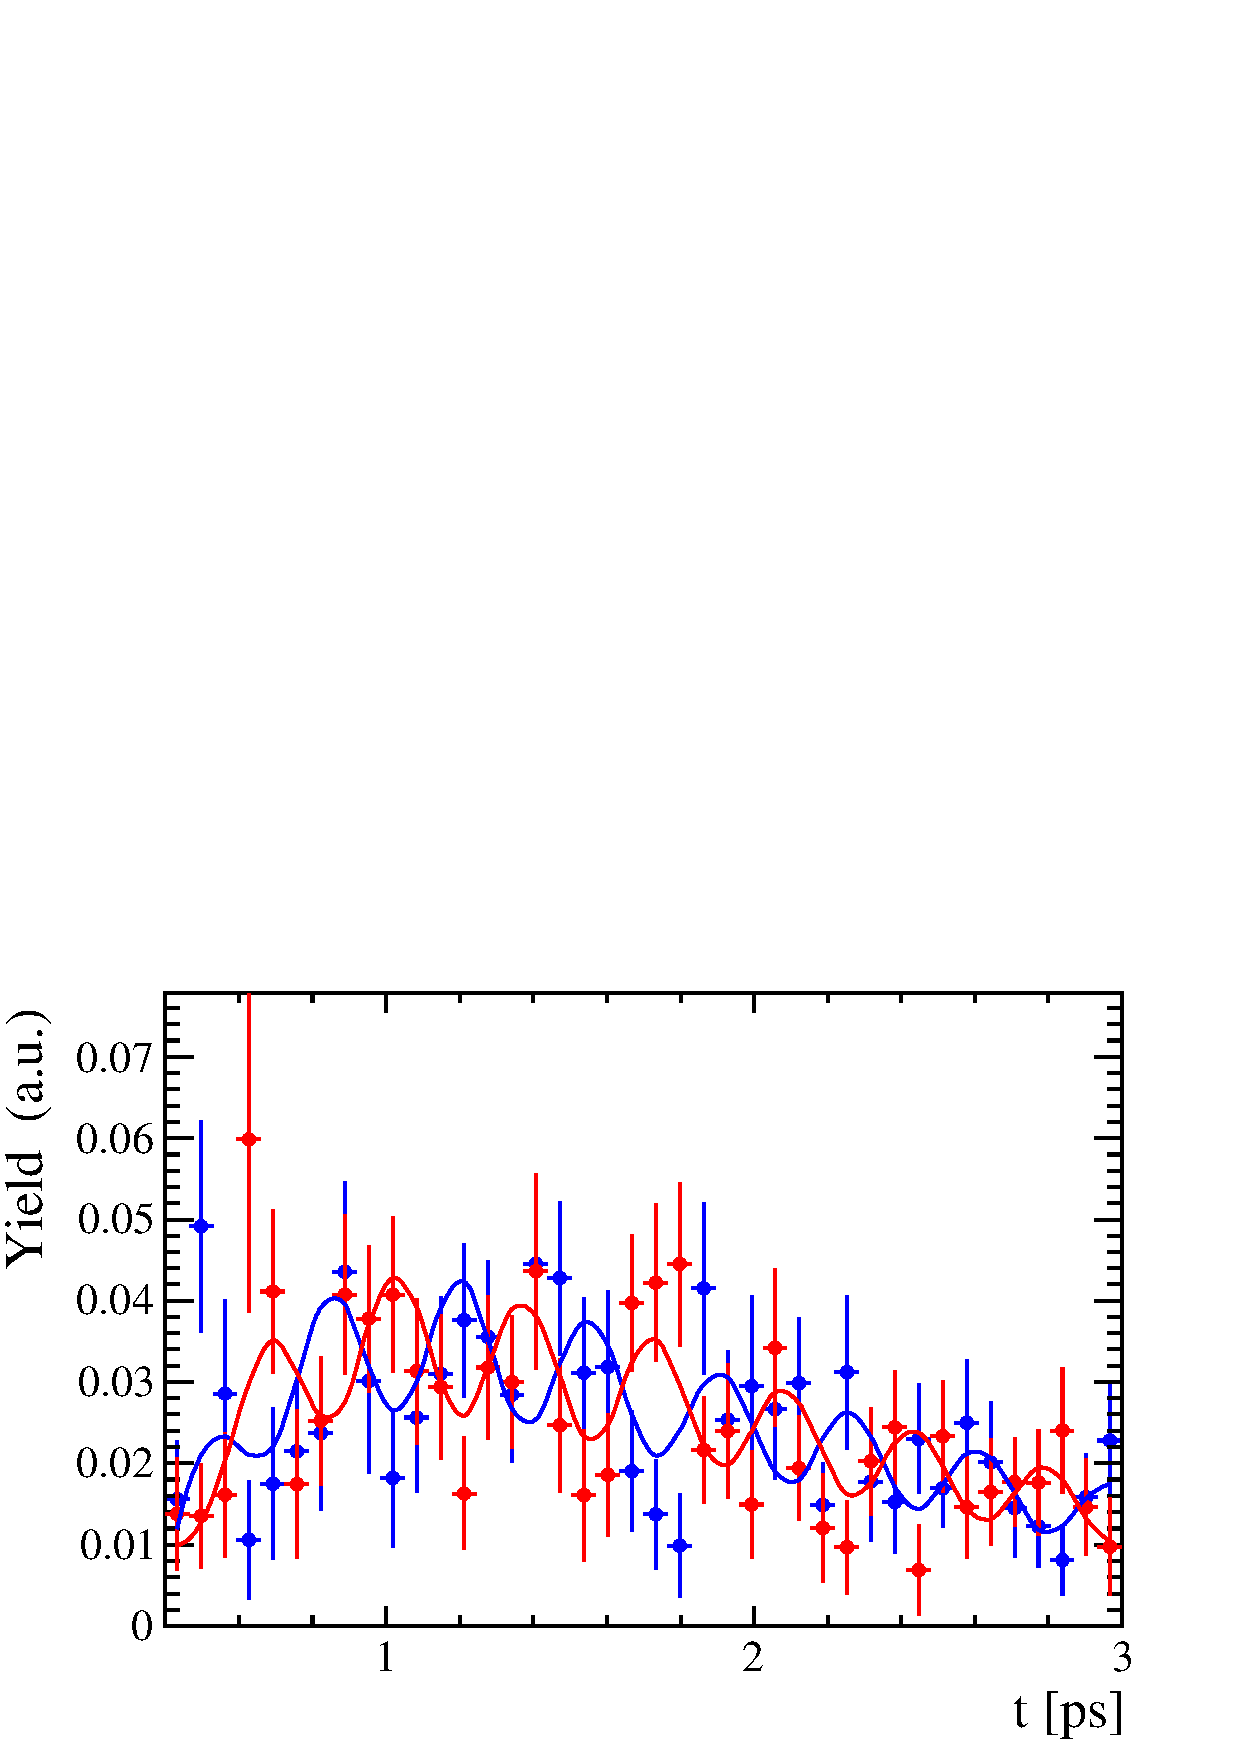
\includegraphics[width=0.32\textwidth, height = !]{figs/timeFit/signal_DsKpipi_CPV_MC/h_t_mixed_m.pdf} 	
		%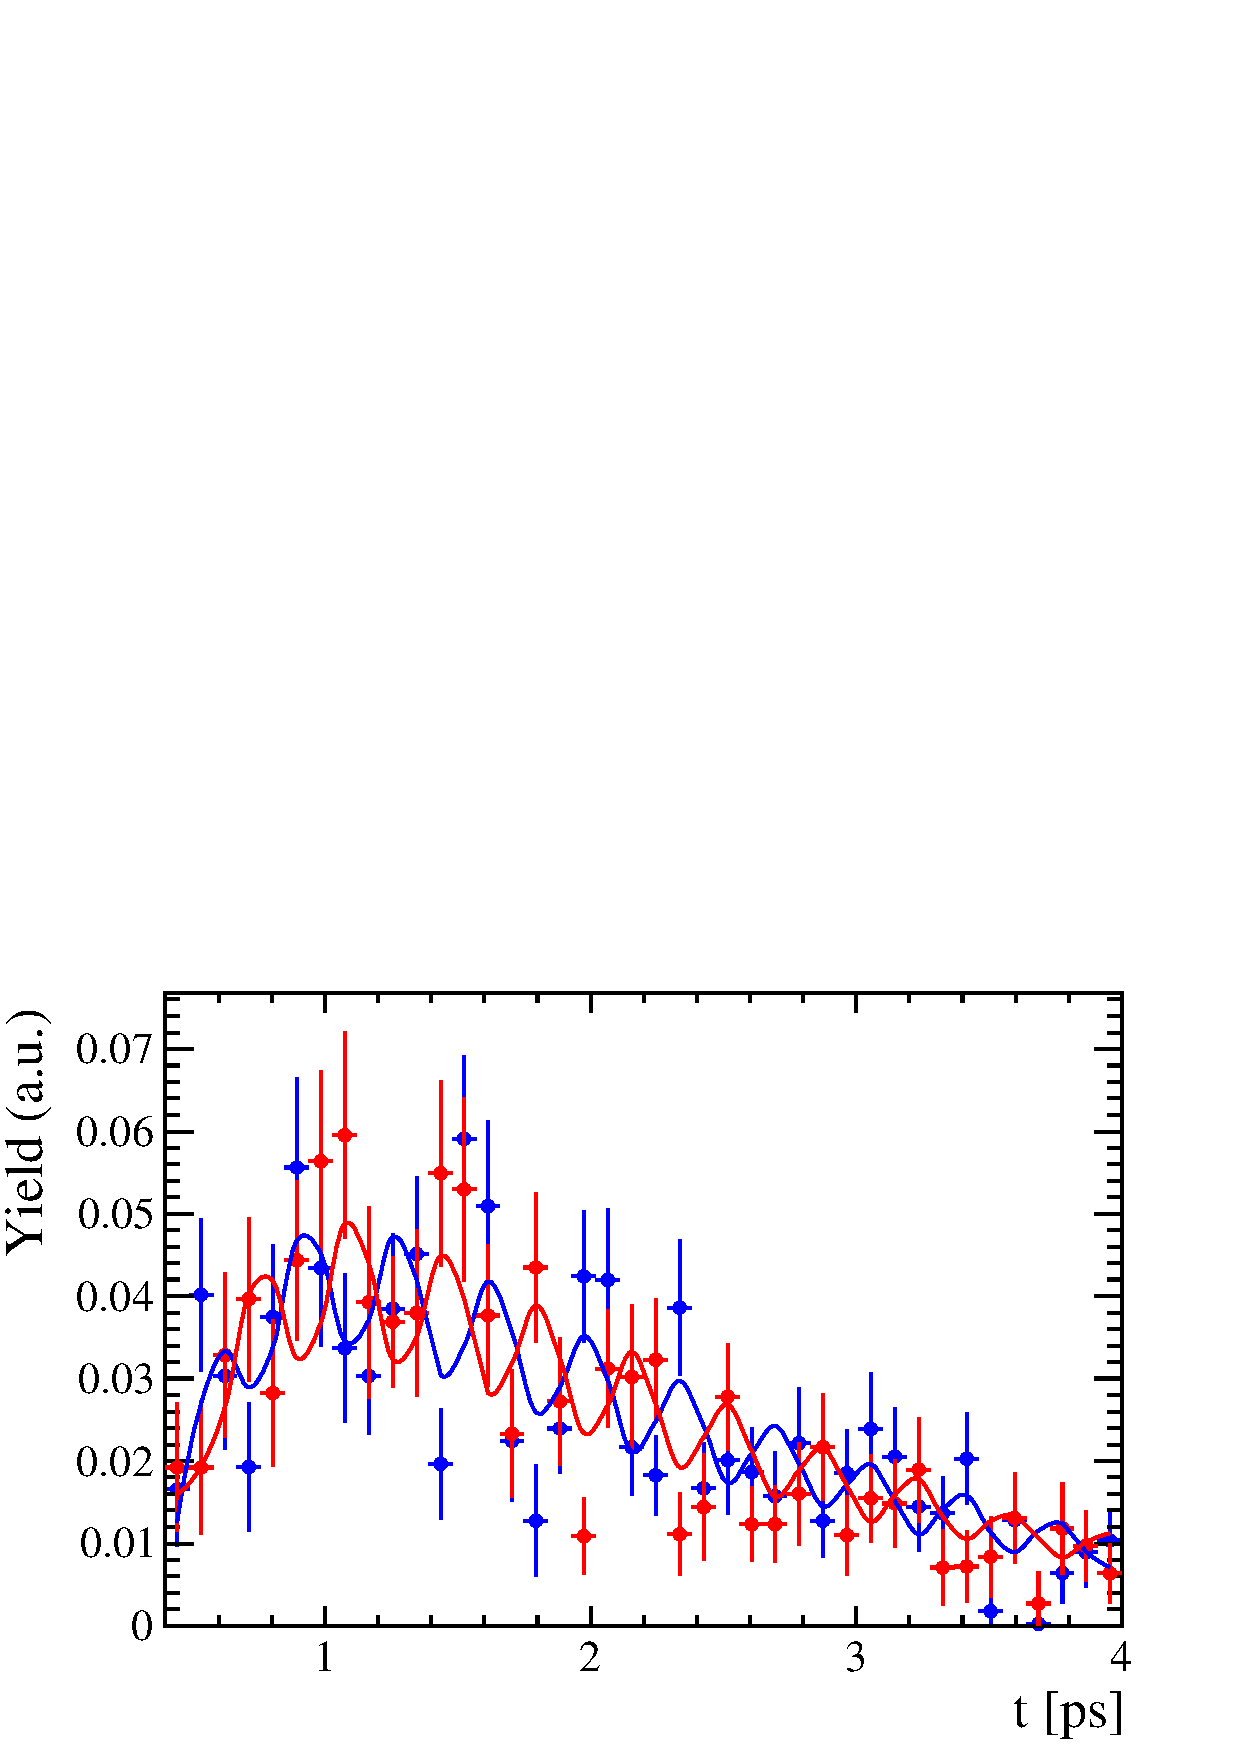
\includegraphics[width=0.32\textwidth, height = !]{figs/timeFit/signal_DsKpipi_CPV_MC/h_t_mixed_p.pdf} 
		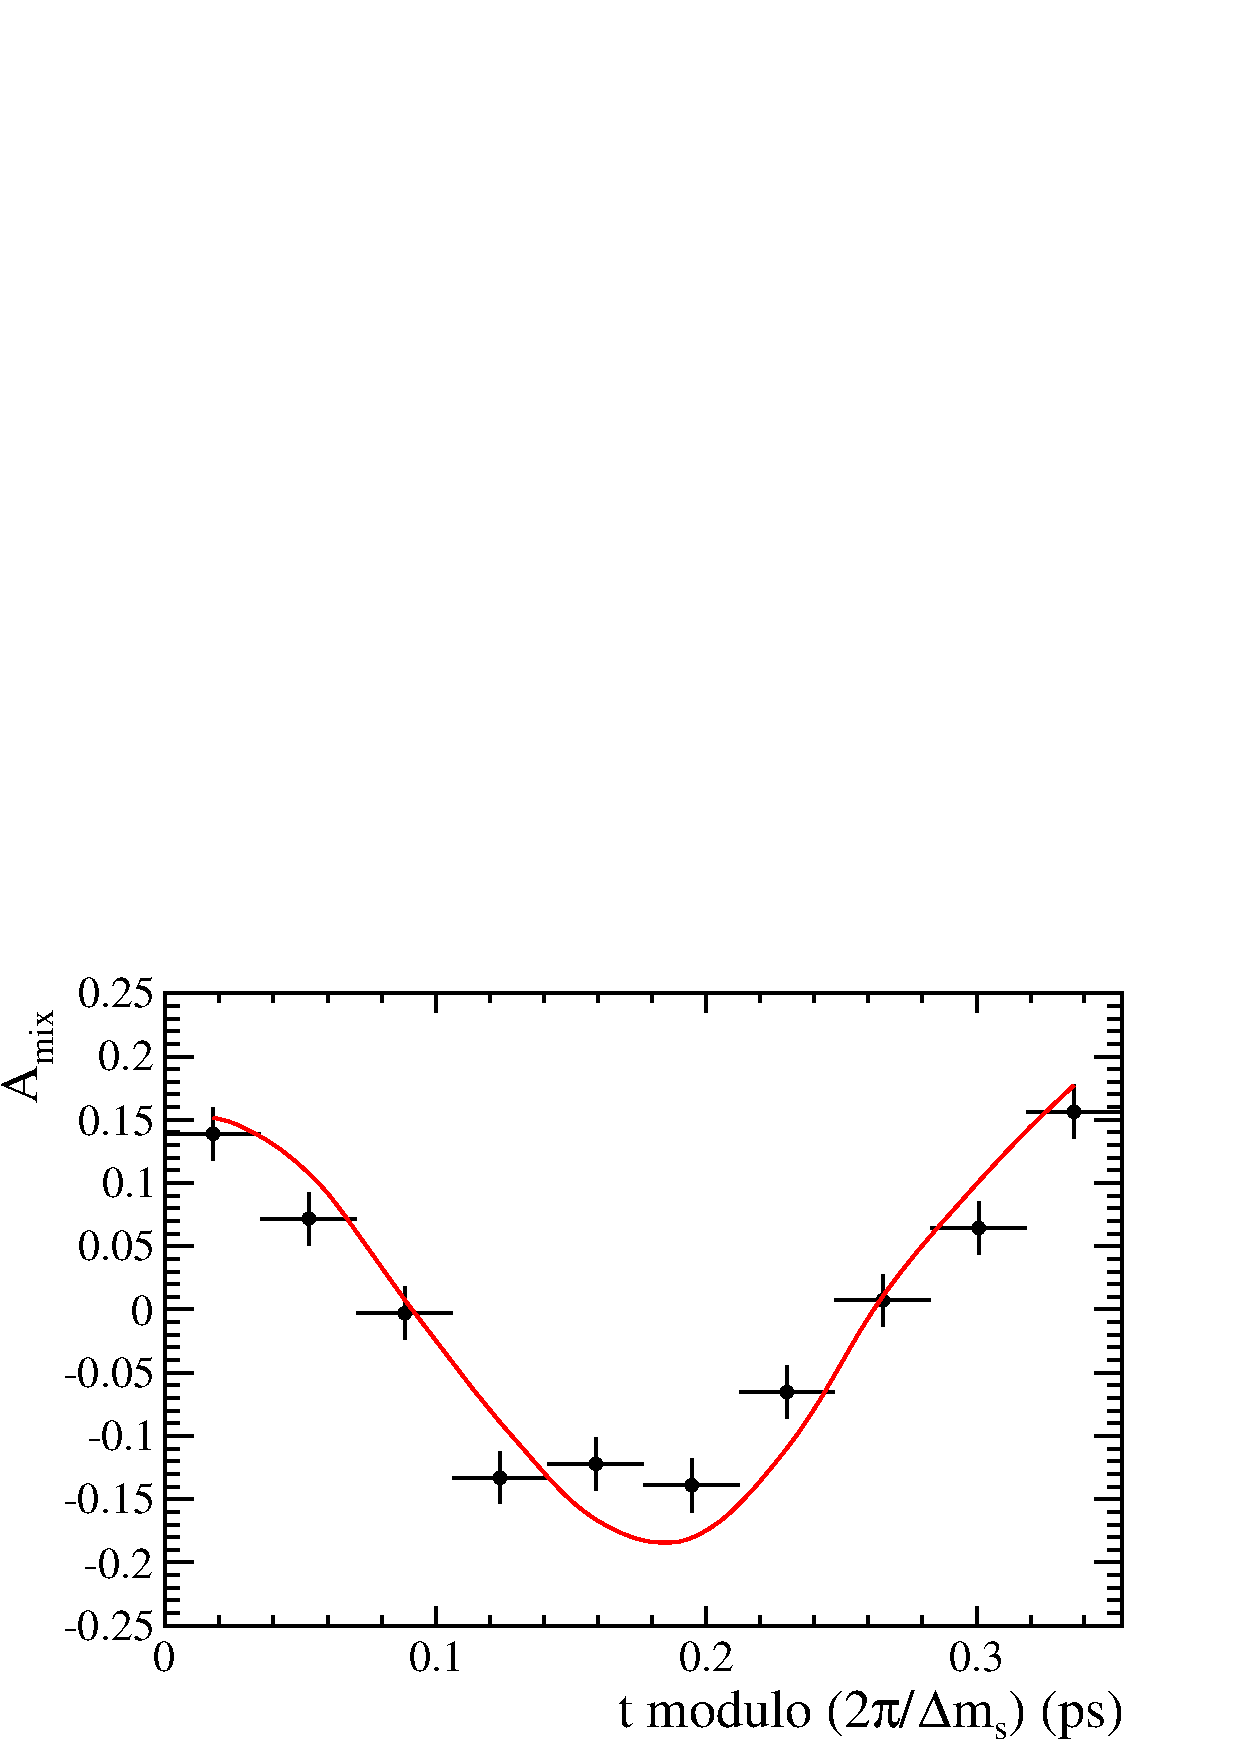
\includegraphics[width=0.45\textwidth, height = !]{figs/timeFit/signal_DsKpipi_CPV_MC/h_asym.pdf} 
		
		\caption{Left: Time distribution of $B_s \to D_s K \pi\pi$ events generated with \textsf{EVTGEN} (points with error bars) and \textsf{MINT2} fit projections (solid line). 
                  Right: Time-dependent asymmetry between mixed and unmixed events folded into one oscillation period for 
                  $D_s^- K^+ \pi\pi$ (red) and $D_s^+ K^- \pi\pi$ (blue) final states.
                  The data points show events generated with \textsf{EVTGEN}, while the solid lines show the \textsf{MINT2} fit projections.}
		\label{fig:FitGenMC}	
\end{figure}	

\begin{figure}[h]
	\centering
		\includegraphics[width=0.32\textwidth, height = !]{figs/fullFit/signal_DsKpipi_CPV_MC/h_t.pdf} 
		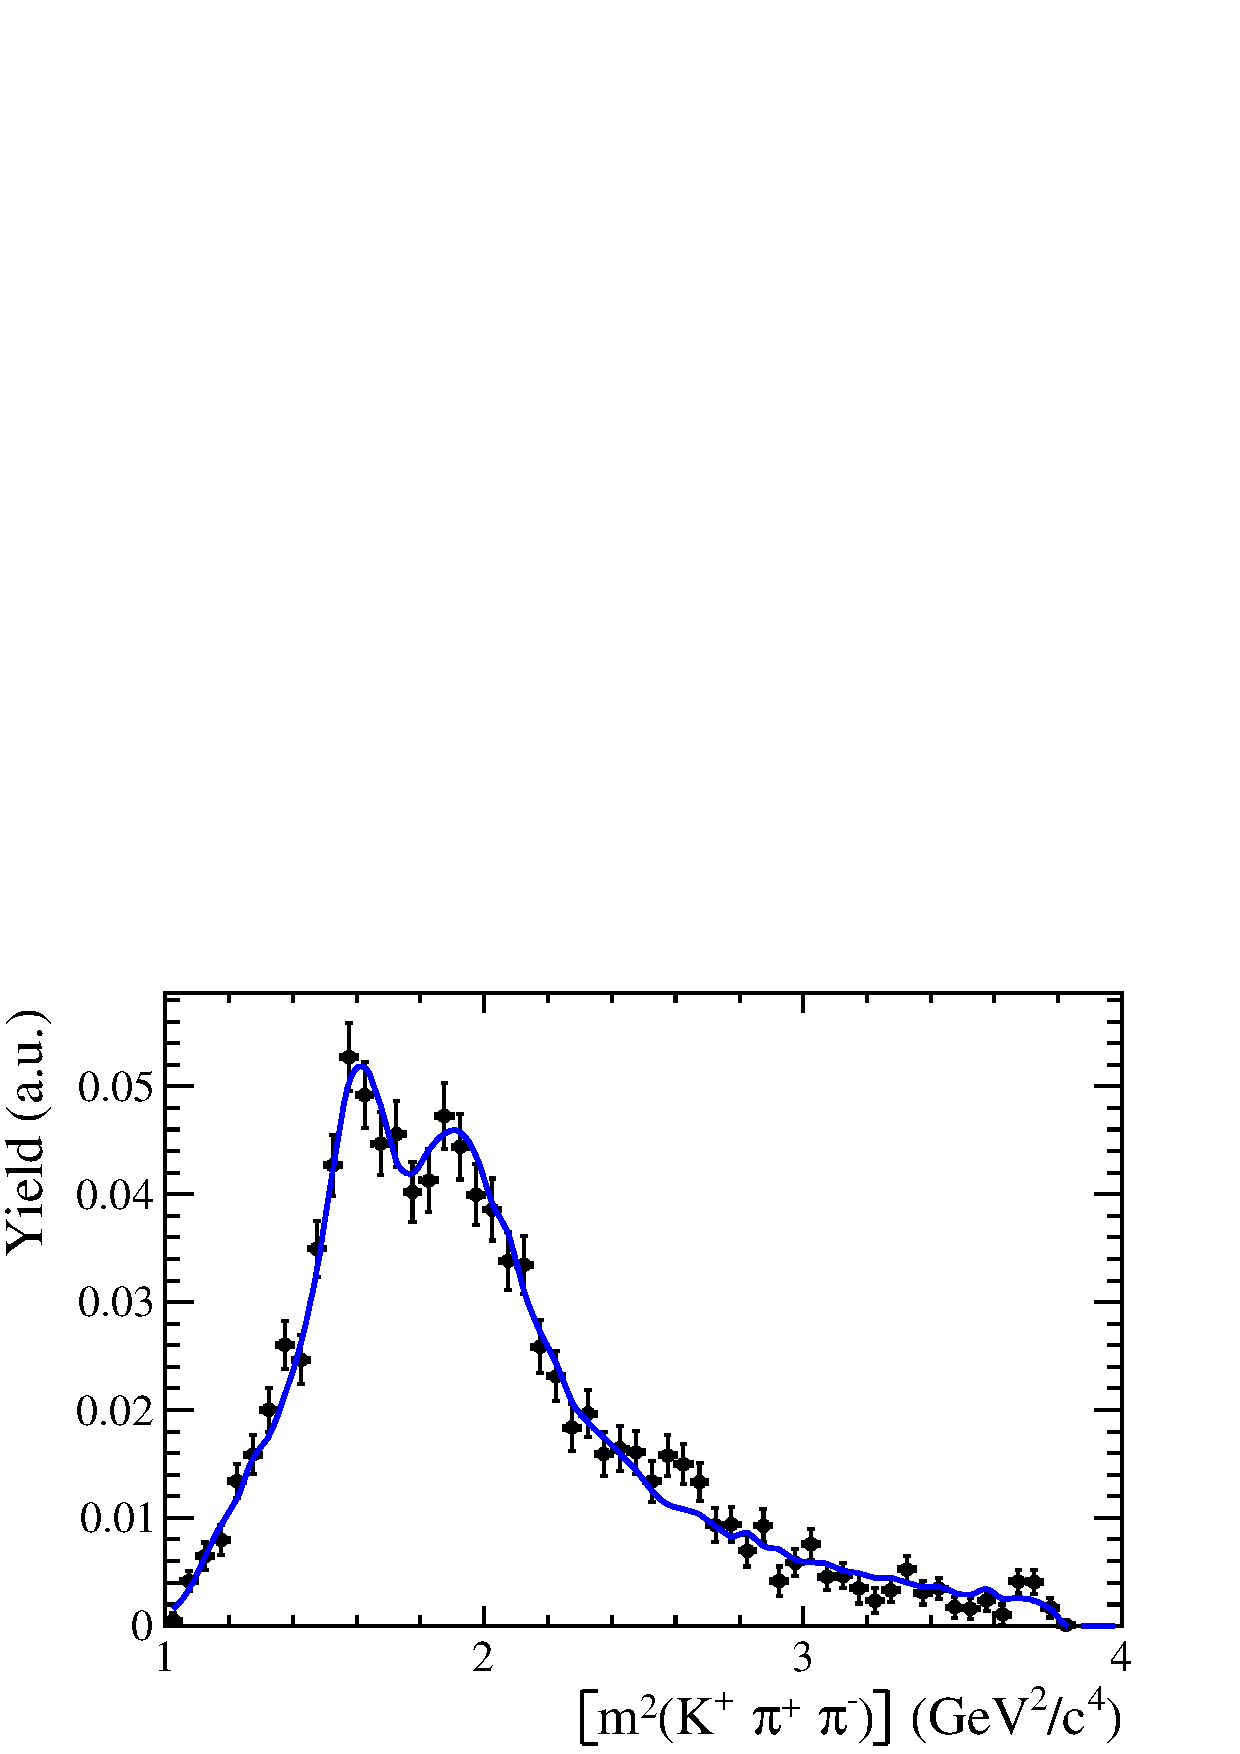
\includegraphics[width=0.32\textwidth, height = !]{figs/fullFit/signal_DsKpipi_CPV_MC/s_Kpipi.pdf} 
		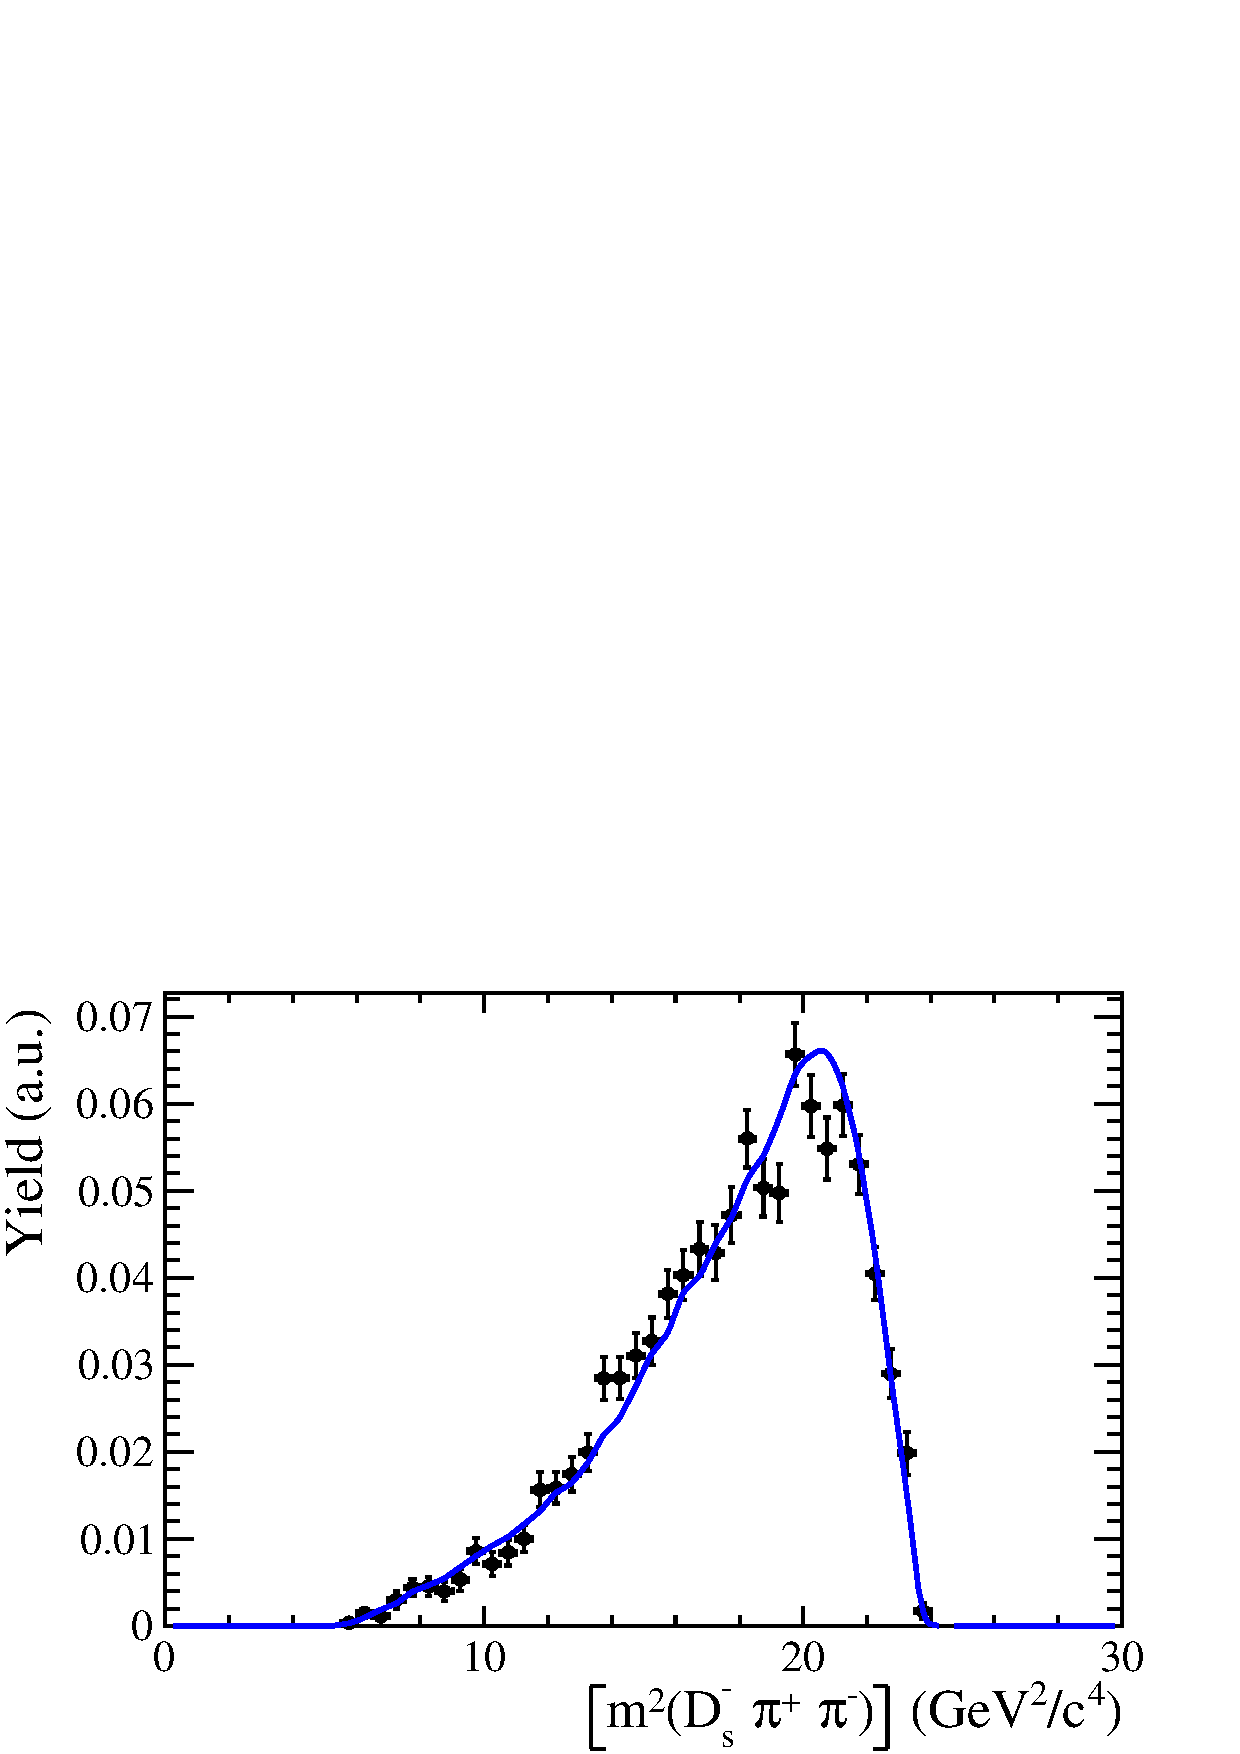
\includegraphics[width=0.32\textwidth, height = !]{figs/fullFit/signal_DsKpipi_CPV_MC/s_Dspipi.pdf} 

		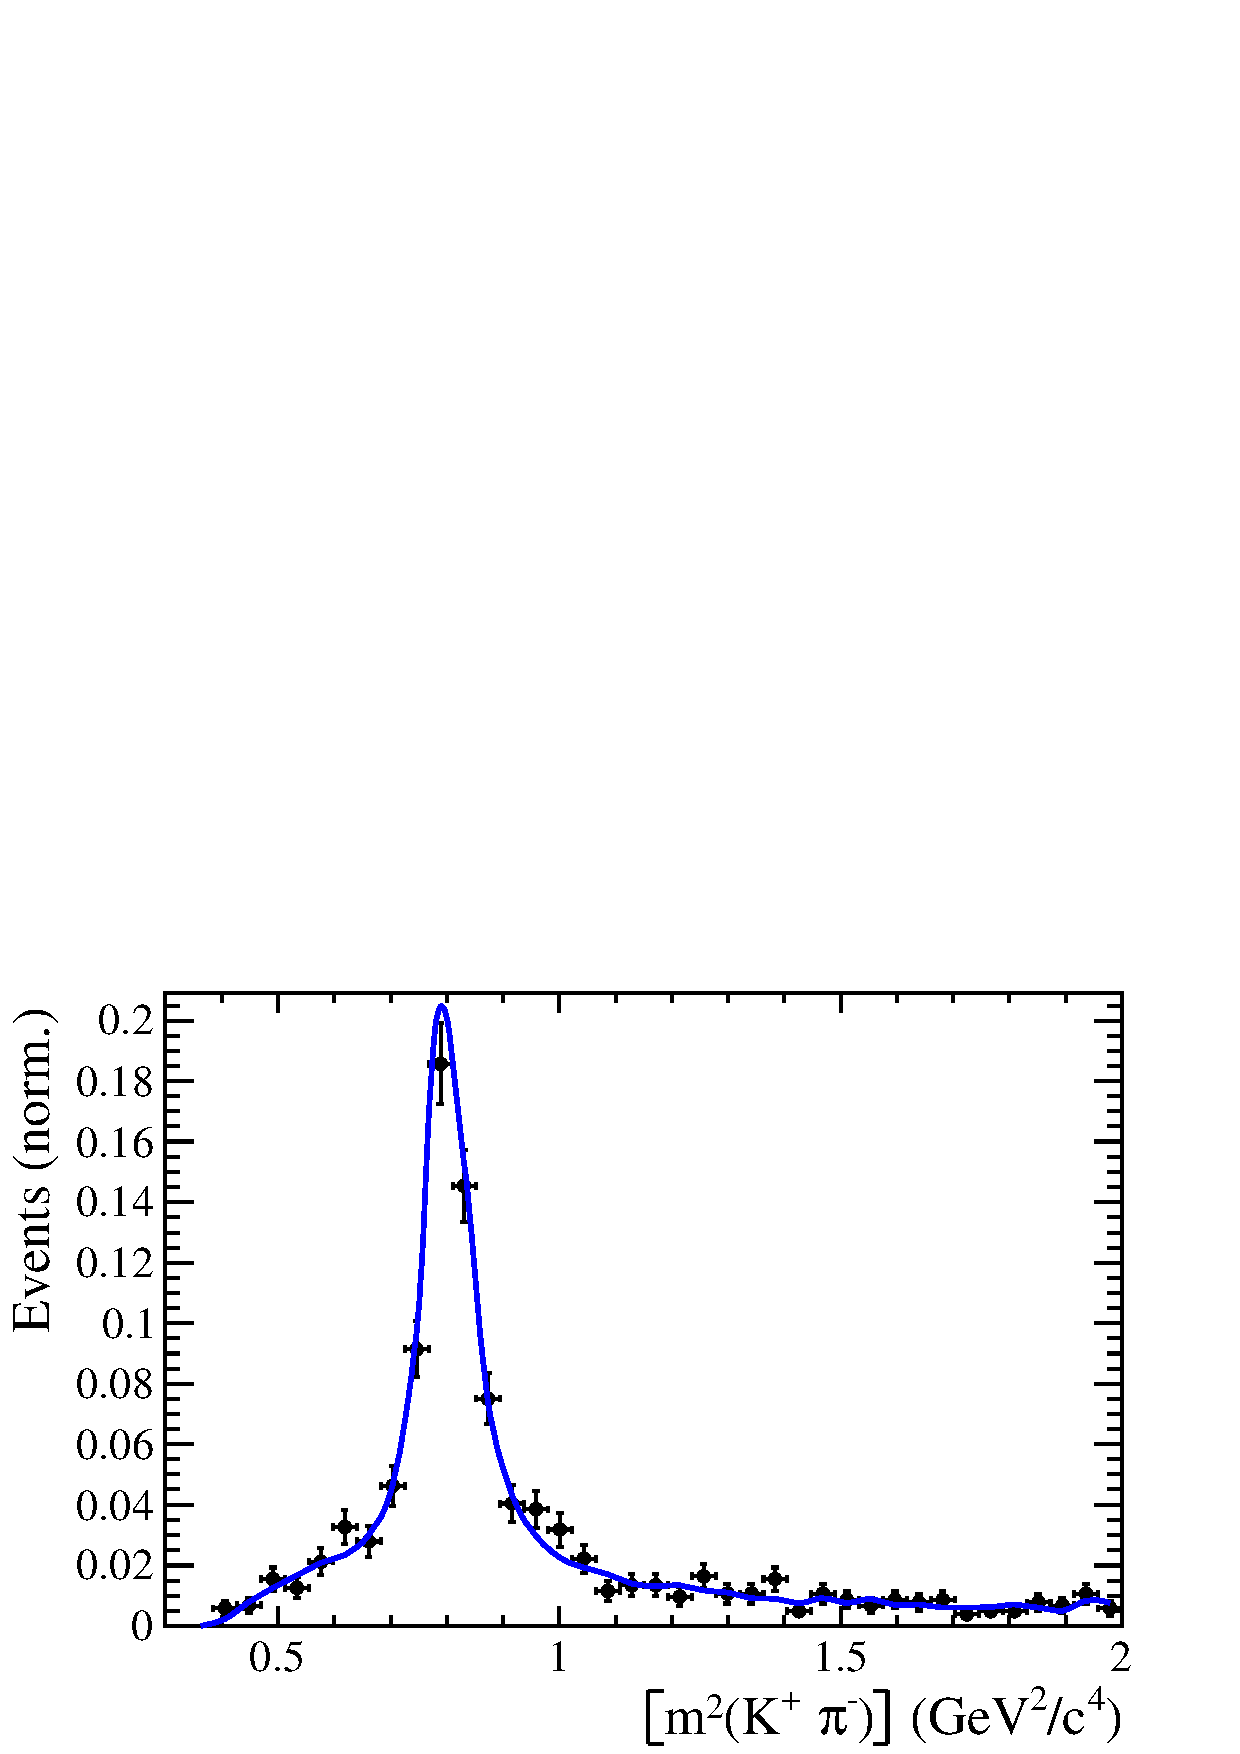
\includegraphics[width=0.32\textwidth, height = !]{figs/fullFit/signal_DsKpipi_CPV_MC/s_Kpi.pdf} 
		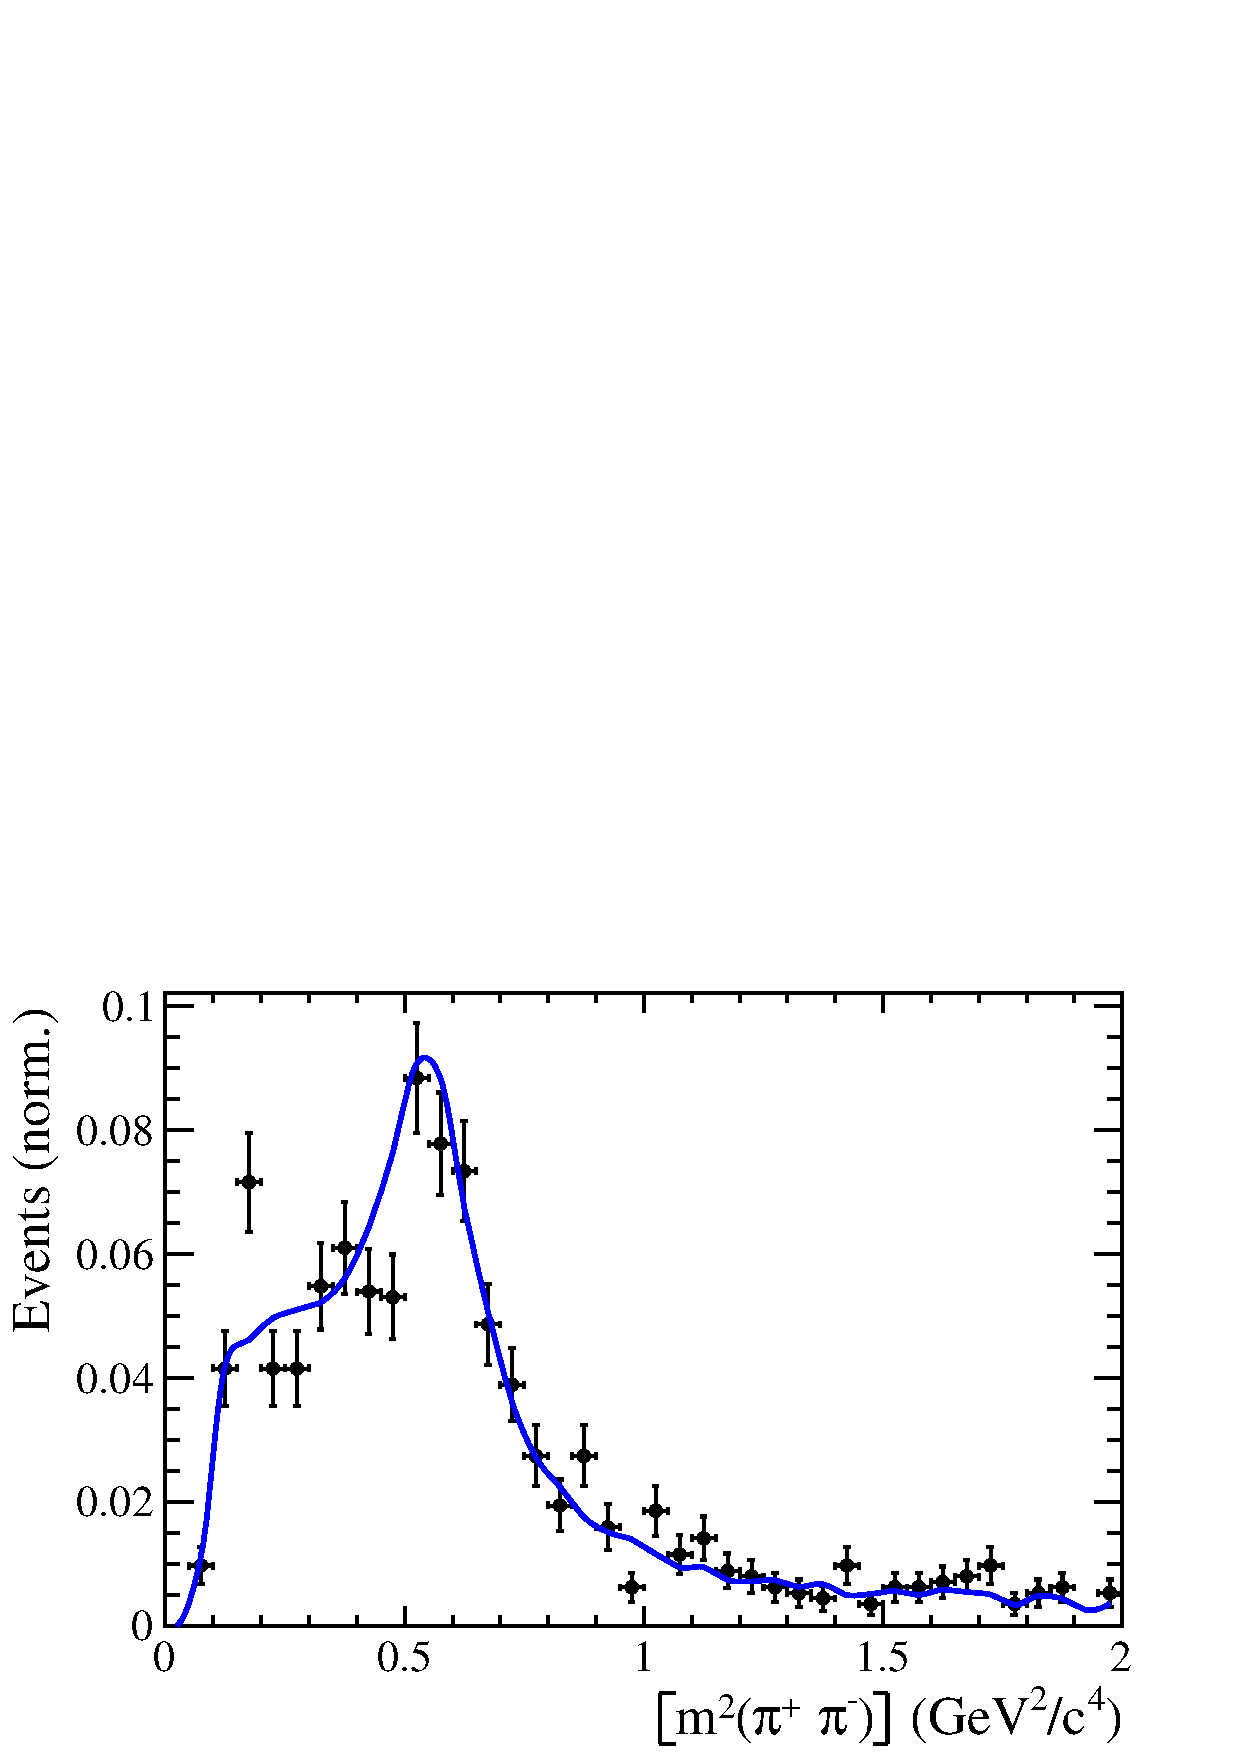
\includegraphics[width=0.32\textwidth, height = !]{figs/fullFit/signal_DsKpipi_CPV_MC/s_pipi.pdf} 
		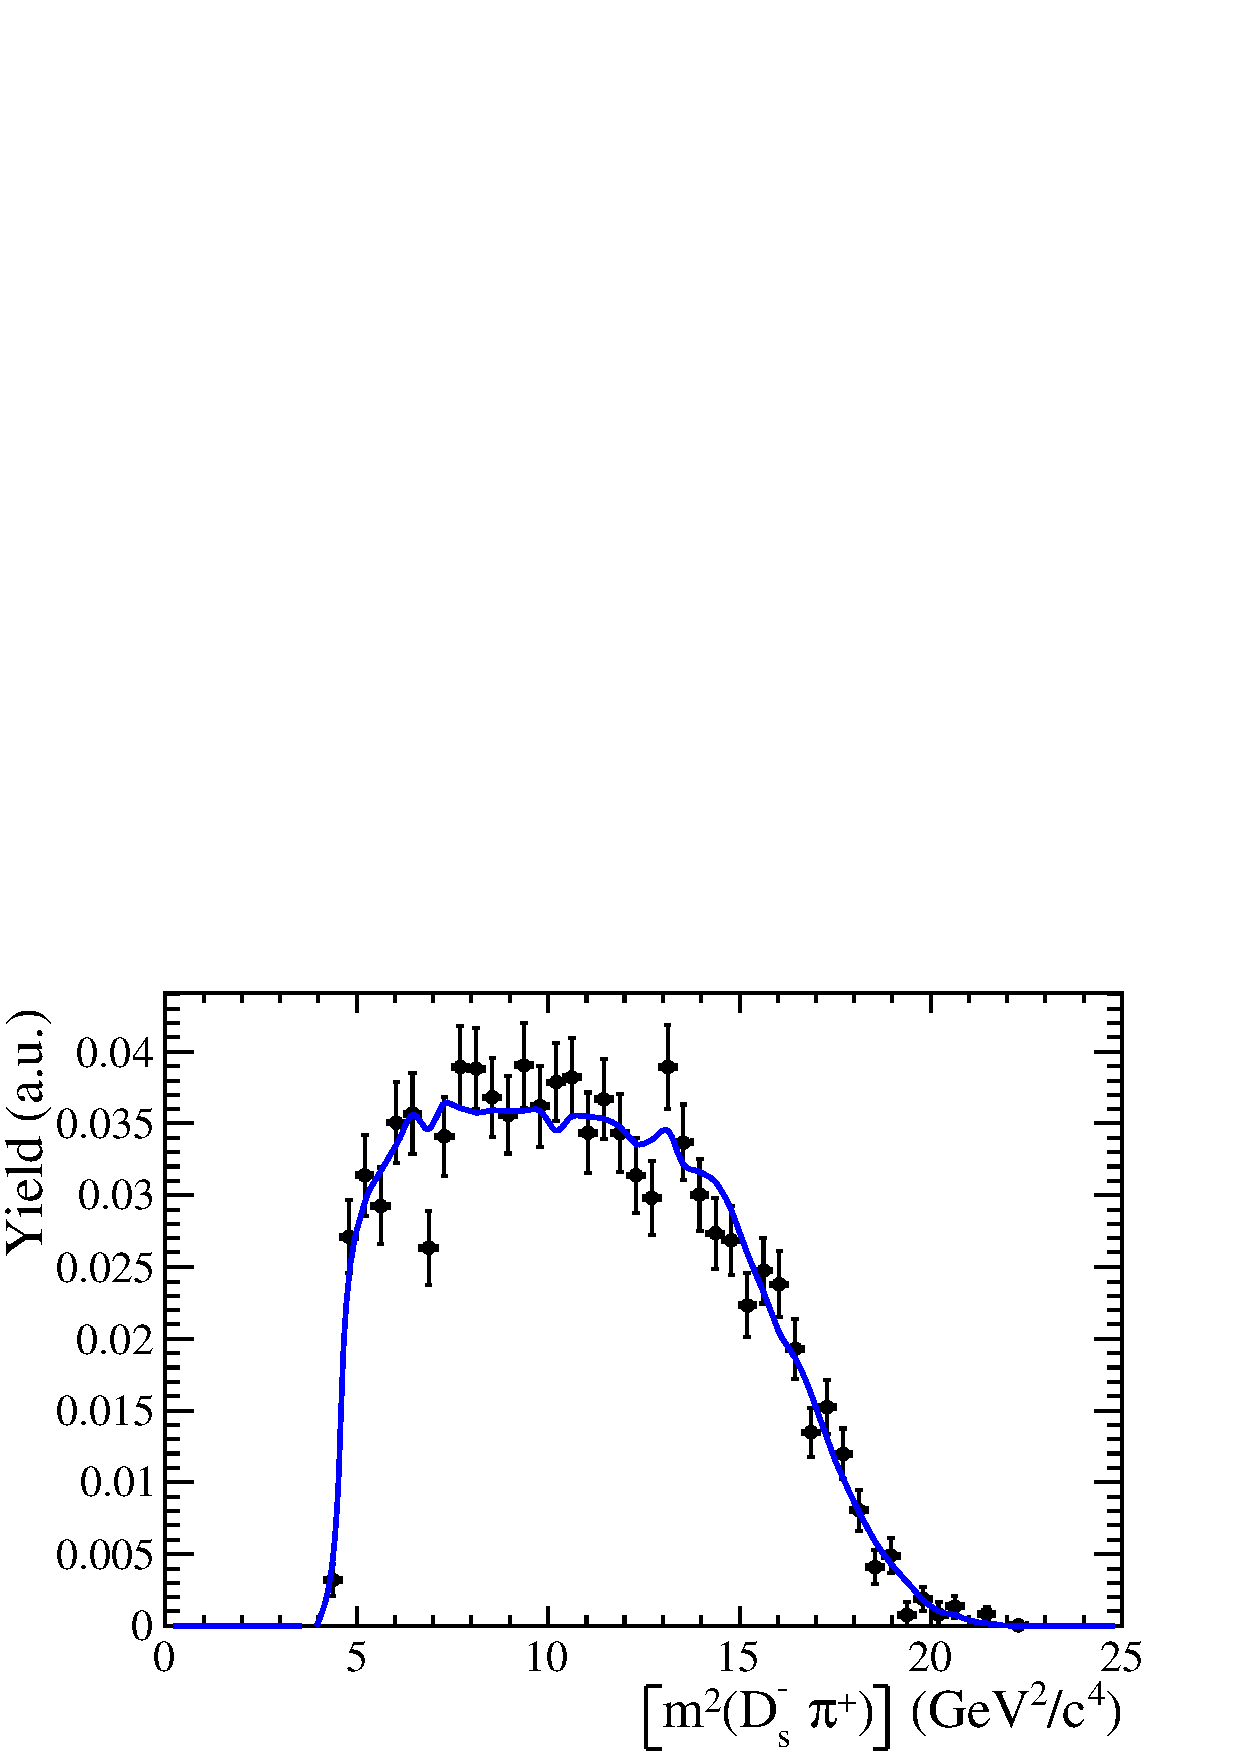
\includegraphics[width=0.32\textwidth, height = !]{figs/fullFit/signal_DsKpipi_CPV_MC/s_Dspi.pdf} 
		
		\caption{Time and invariant mass distributions of $B_s \to D_s K \pi\pi$ events generated with \textsf{EVTGEN} (points with error bars) and \textsf{MINT2} fit projections (blue solid line).} 		
		\label{fig:FitGenMC2}	
\end{figure}	

\begin{figure}[h]
	\centering
		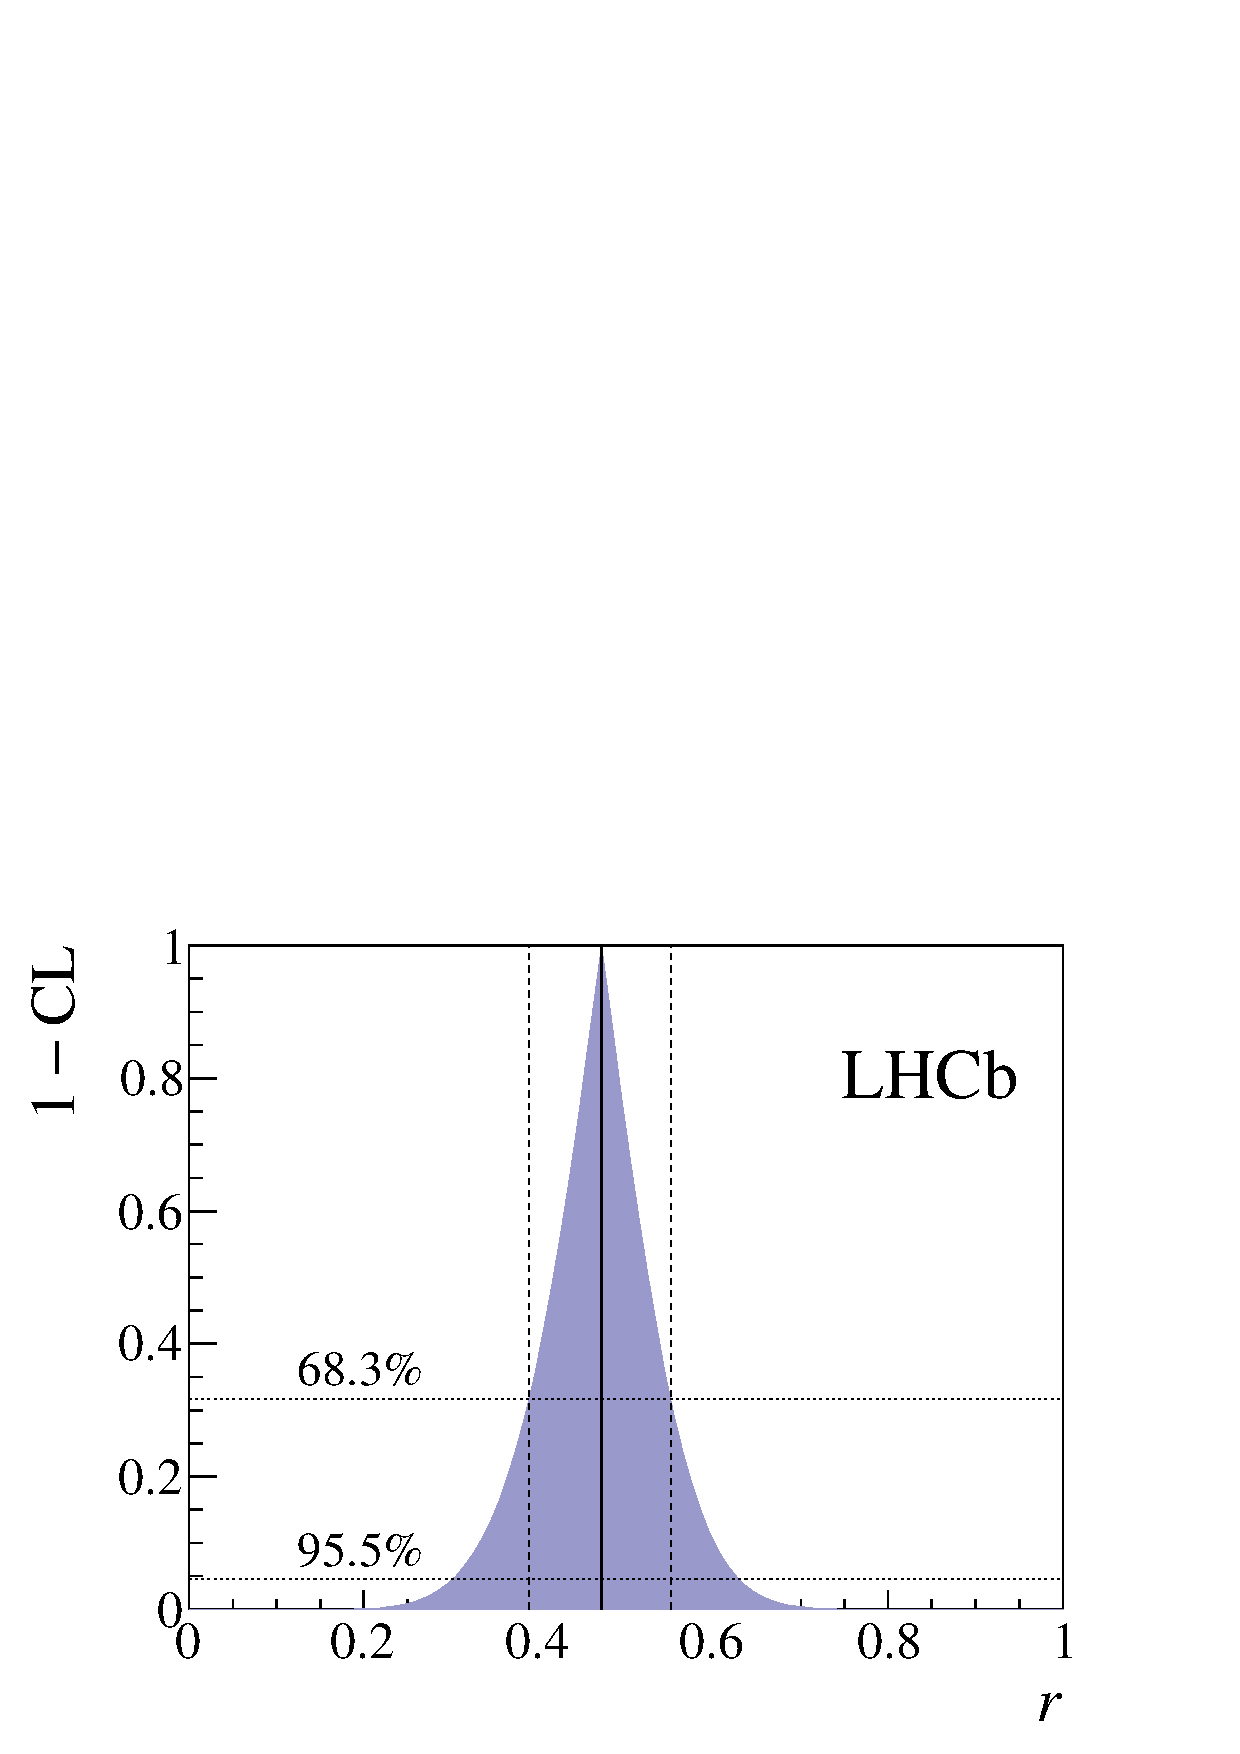
\includegraphics[width=0.4\textwidth, height = !]{figs/GammaCombo/signal_DsKpipi_CPV_MC/cartesian_cp_coeff_r.pdf} 
		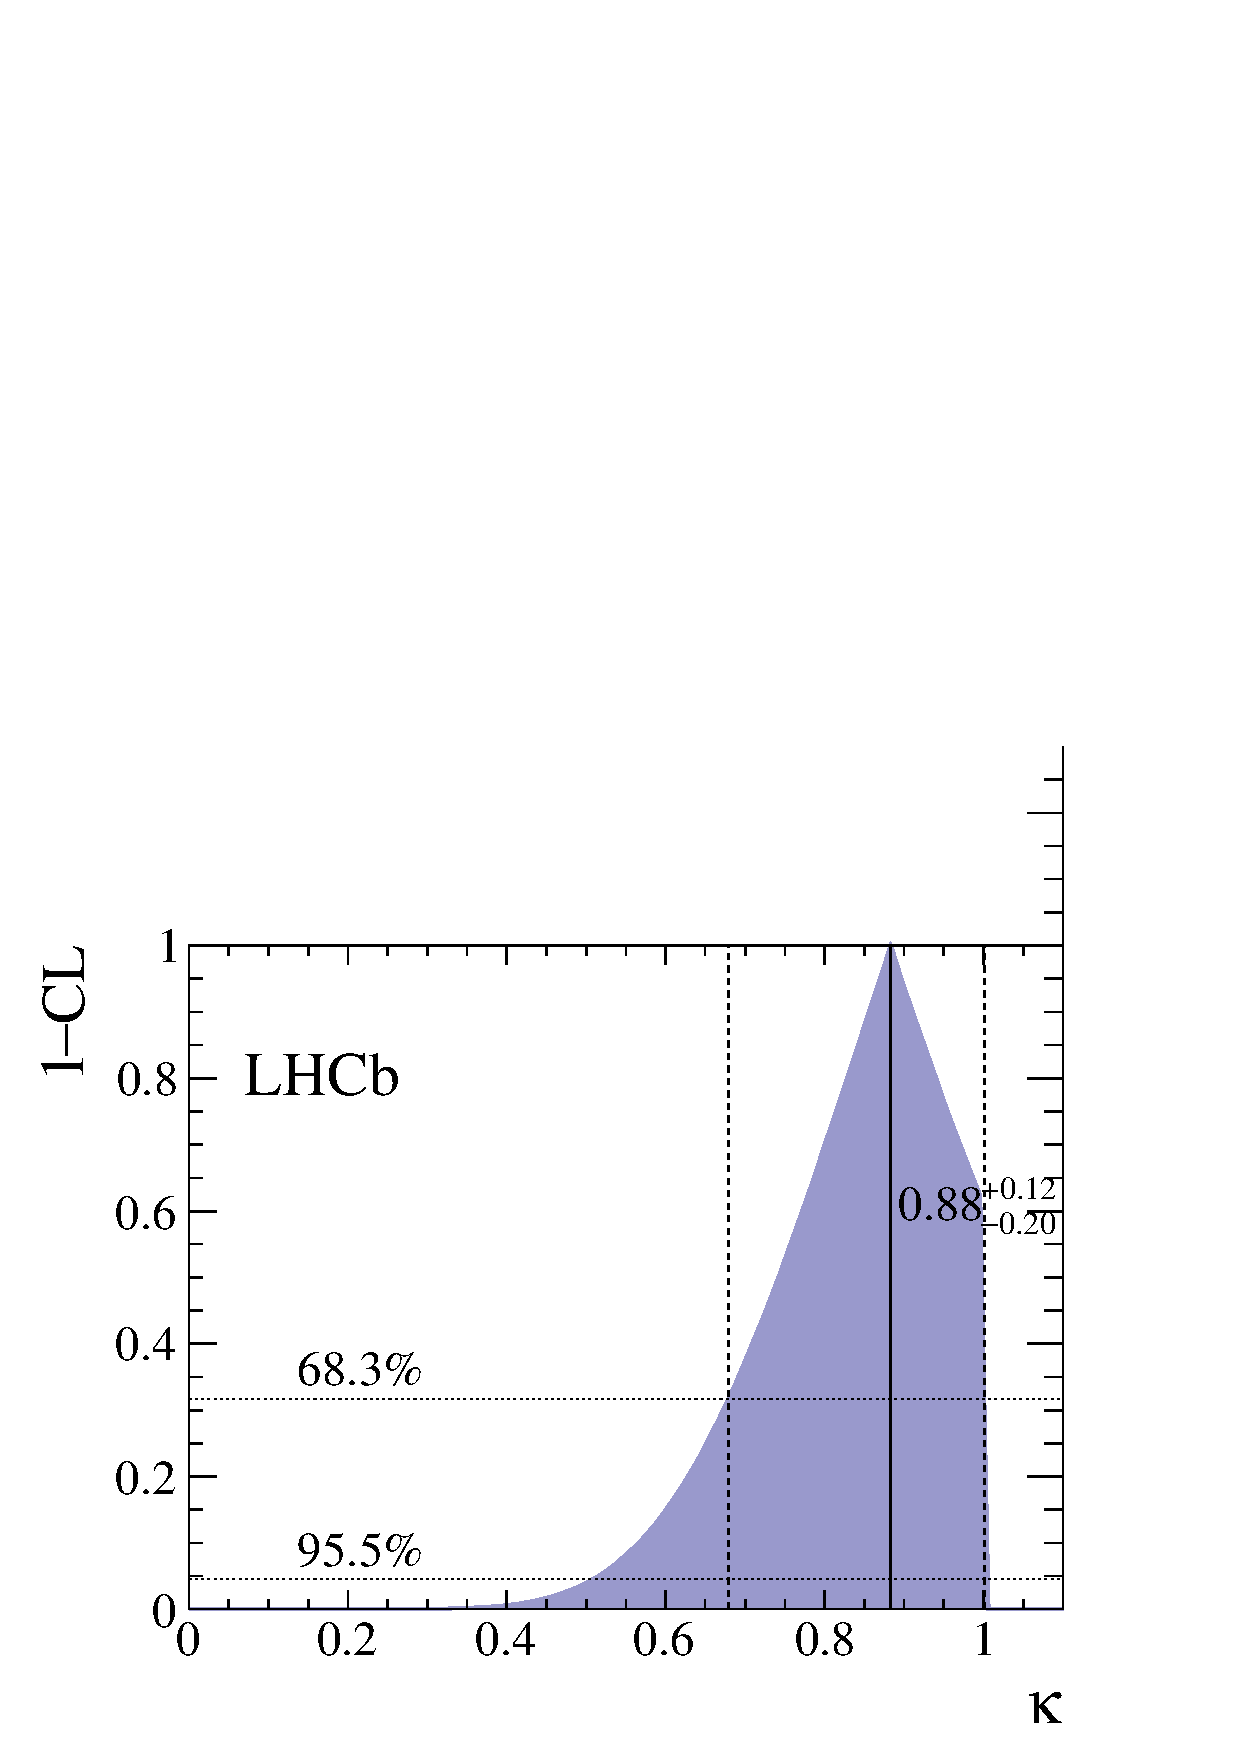
\includegraphics[width=0.4\textwidth, height = !]{figs/GammaCombo/signal_DsKpipi_CPV_MC/cartesian_cp_coeff_k.pdf} 
		
		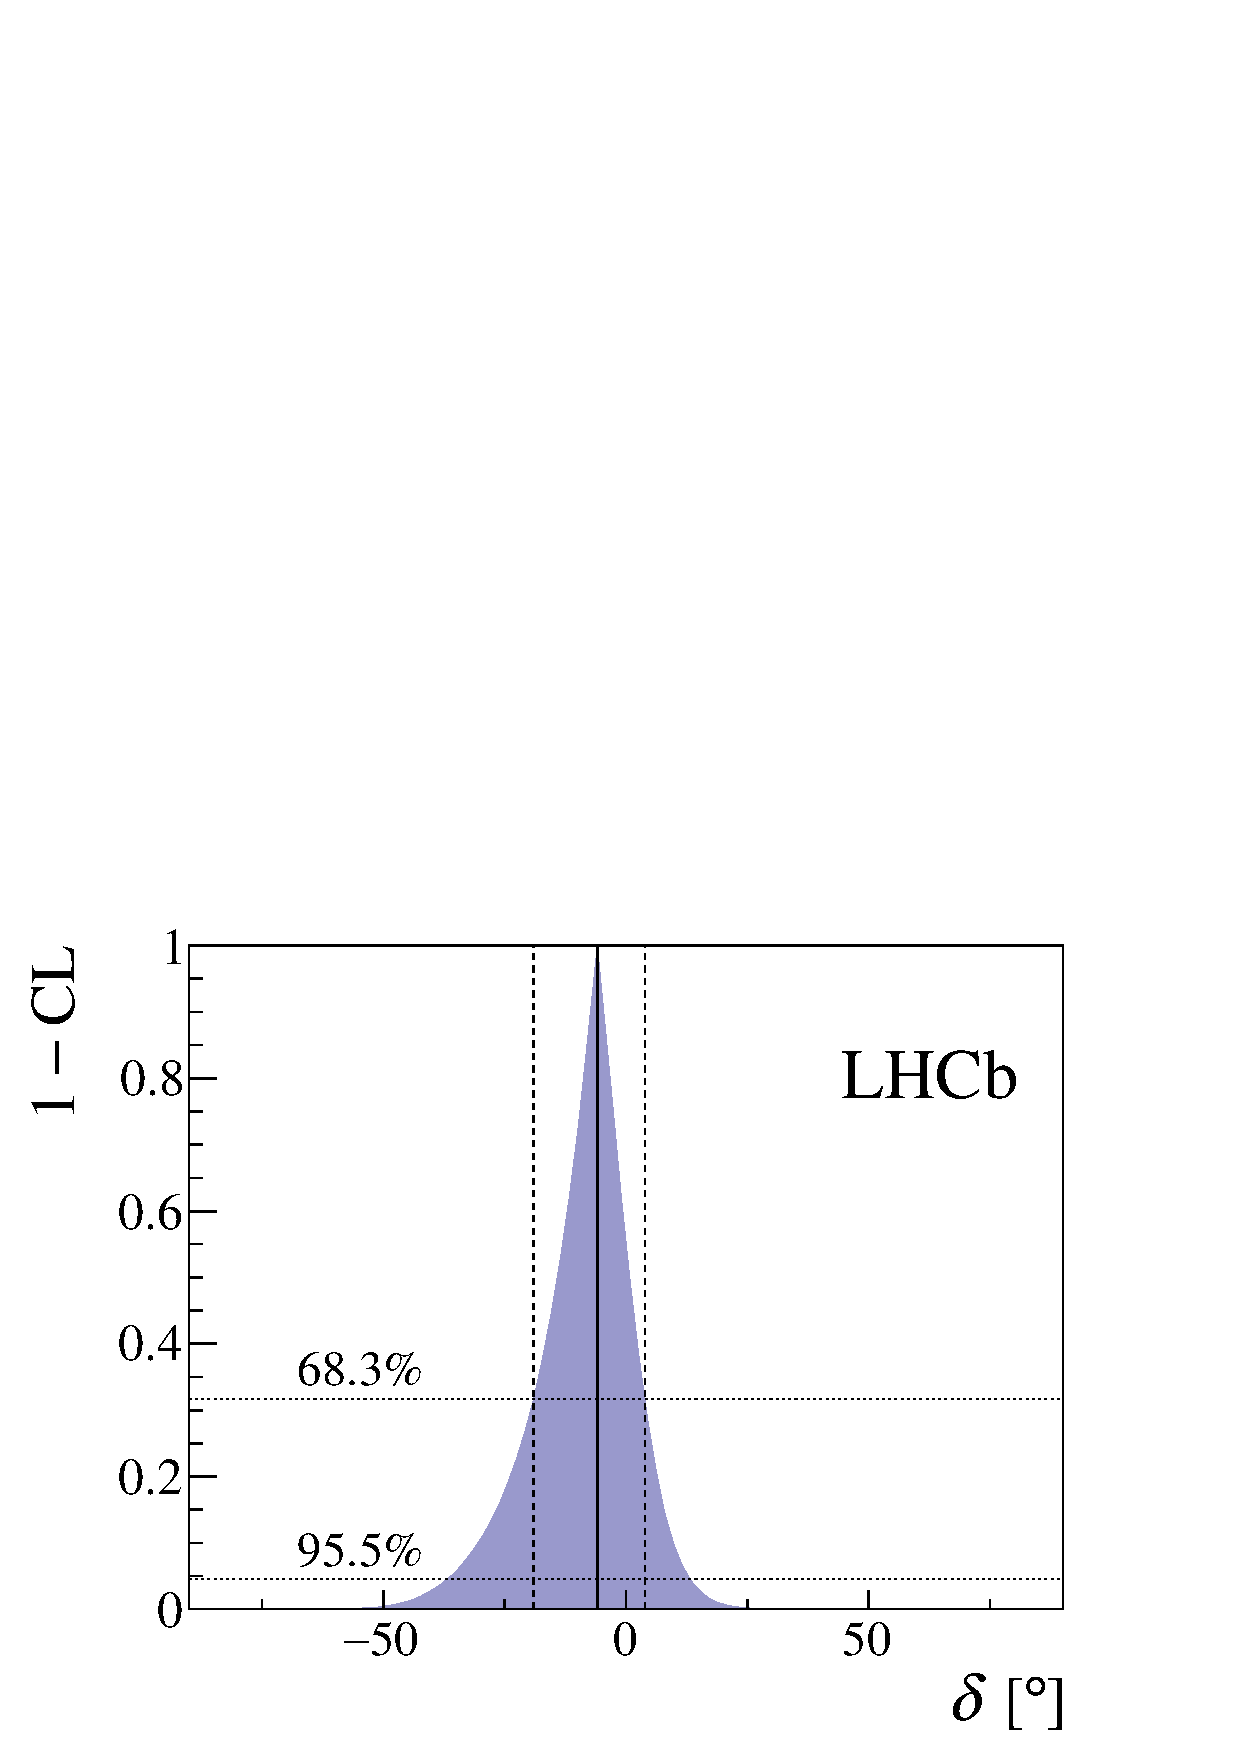
\includegraphics[width=0.4\textwidth, height = !]{figs/GammaCombo/signal_DsKpipi_CPV_MC/cartesian_cp_coeff_d.pdf} 
		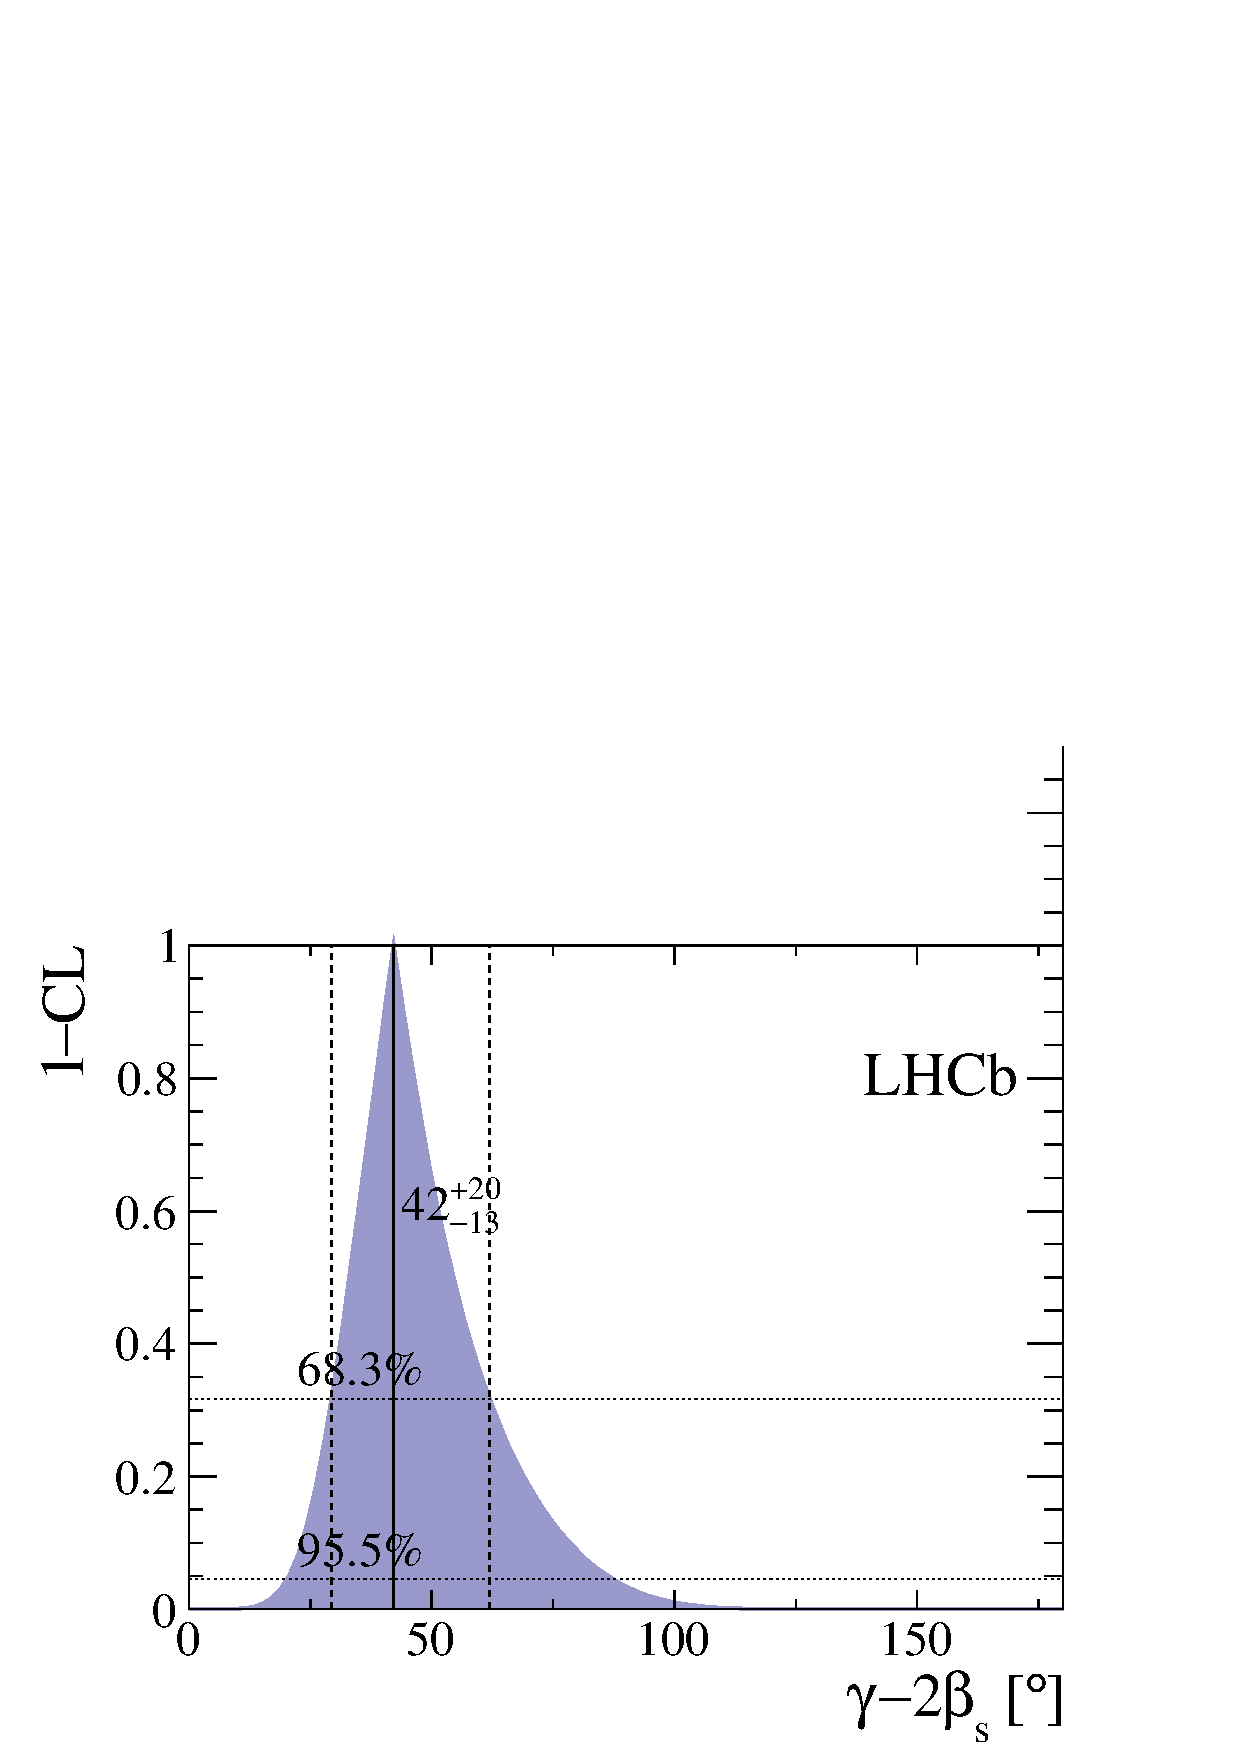
\includegraphics[width=0.4\textwidth, height = !]{figs/GammaCombo/signal_DsKpipi_CPV_MC/cartesian_cp_coeff_g.pdf} 
		\caption{The 1-CL contours for the physical observable $r,\kappa,\delta$ and $\gamma$ obtained with the phasespace-integrated fit to the \textsf{EVTGEN} toy sample. }
		\label{fig:FitGenCL}	
\end{figure} 

\begin{table}[h]
\caption{Result of the phasespace-integrated fit to \textsf{EVTGEN} toy events.} 		
%\resizebox{0.45\linewidth}{!}{
%  \scriptsize
  \centering
  \begin{tabular}
    {l c c c}
    \hline \hline
    & Generated &  Fit result  & Pull($\sigma$) \\   \hline
    $C$ & 0.759  &  $0.767 \pm 0.023 $  & 0.3         \\
    $D$ &  -0.314 &  $-0.194 \pm 0.205$ & 0.6         \\
    $\bar D$ &  -0.101 &  $-0.189 \pm 0.210$ & -0.4   \\
    $S$ &   -0.570 &  $-0.556 \pm 0.033$     & 0.4 \\
    $\bar S$ &  -0.643   &  $-0.683\pm 0.031$ & -1.3  \\
    \hline \hline
  \end{tabular}
    \label{tab:FitGenMC}
%    }
\end{table}

%\begin{table}[h]
%\caption{Result of the time-dependent amplitude fit to \textsf{EVTGEN} toy events.} 		
%%   \resizebox{0.45\linewidth}{!}{ 
%%  \scriptsize
%  \centering
%  \begin{tabular}
%    {l c c c}
%    \hline \hline
%    & Generated &  Fit result & Pull($\sigma$) \\   \hline
%    $x_-$ & 0.179  &  $0.135 \pm 0.050$ & -0.9	 \\
%    $y_-$ &  -0.324 & $-0.307 \pm 0.022$ 	& 0.8 \\
%    $x_+$ &  0.057 & $0.102 \pm 0.065$ & 0.6	 \\
%    $y_+$ &   0.366 &  $0.394 \pm 0.023$	& 1.3 \\
%    \hline \hline
%  \end{tabular}
%    \label{tab:FitGenMC2}
%%    }
%\end{table}

\begin{table}[h]
\caption{Results for the physical observables obtained from fits to \textsf{EVTGEN} toy events.} 		
%  \scriptsize
  \centering
  \begin{tabular}
    {l c c c c}
    \hline \hline
    & Generated &  Full PDF     &   Phasespace-integrated  \\   \hline
 $r$ & 0.370 & $0.372 \pm 0.015 $ & $0.372 \pm 0.015$  \\
 $\kappa$  &1.0 & 1.0 &  $1.000 \pm  0.035$  \\
 $\delta$ & $10.0^\circ$ &  $12.2 \pm  5.1$ & $12.3 \pm  5.1$   \\
 $\gamma$ & $71.1^\circ$ &   $73.2 \pm 5.5$ &  $73.4 \pm 5.5$\\
    \hline \hline
  \end{tabular}
      \label{tab:FitGenMC3}
\end{table}

      

%\begin{figure}[h]
%	\centering
%		\includegraphics[width=0.4\textwidth, height = !]{figs/GammaCombo/signal_DsKpipi_CPV_MC/cartesian_GenMC_r.pdf} 		
%		\includegraphics[width=0.4\textwidth, height = !]{figs/GammaCombo/signal_DsKpipi_CPV_MC/cartesian_GenMC_d.pdf} 
%		
%		\includegraphics[width=0.4\textwidth, height = !]{figs/GammaCombo/signal_DsKpipi_CPV_MC/cartesian_GenMC_g.pdf} 
%		\caption{The 1-CL contours for the physical observable $r,\delta,\gamma$ obtained with the time-dependent amplitude fit fit to the \textsf{EVTGEN} toy sample. } 	
%\end{figure}  
    


\clearpage
% !TEX root = main.tex

\section{Data samples and event selection}
\label{sec:Selection}

%Throughout the note, we abbreviate $\Bs\to\Ds X_{s}(\to\kaon\pion\pion)$ and $\Bs\to\Ds X_{d}(\to\pion\pion\pion)$. 
%, identifying $X_{s}\to\kaon\pion\pion$ and $X_{d}\to\pion\pion\pion$ as the various resonances through which the decays proceed. 

\subsection{Stripping and Trigger selection}

The dataset used for this analysis corresponds to $1 \invfb$ of proton-proton collision data
collected in 2011 with a centre of mass energy $\sqrt{s} = 7\tev$,  $2 \invfb$  collected in
2012 with $\sqrt{s} = 7\tev$ and $2 \invfb$  collected in
2015/2016 with $\sqrt{s} = 13\tev$.
Candidate $\Bs\to\Ds\kaon\pion\pion$ ($\Bs\to\Ds\pion\pion\pion$) decays are reconstructed using the
\textsf{B02DKPiPiD2HHHPIDBeauty2CharmLine} (\textsf{B02DPiPiPiD2HHHPIDBeauty2CharmLine})
line of the \textsf{BHadronCompleteEvent} stream of  
\textsf{Stripping21r1} (2011), \textsf{Stripping21} (2012),
\textsf{Stripping24r1} (2015)  and \textsf{Stripping28r1p1} (2016).
%and \textsf{Stripping29r2} (2017)
Both stripping lines employ the same selection cuts, listed in Appendix \ref{sec:StripAndTrigger}, except for the PID requirement on the bachelor kaon/pion.

Events that pass the stripping selection are further required to fulfill the following trigger requirements:
at the hardware stage, the $\Bs$ candidates are required to be TOS on the \textsf{L0Hadron} trigger or TIS on \textsf{L0Global};
at Hlt1, $\Bs$ candidates are required to be TOS on the \textsf{Hlt1TrackAllL0} (\textsf{Hlt1TrackMVA} or \textsf{Hlt1TwoTrackMVA}) trigger line for Run-I (Run-II) data;
at Hlt2, candidates have to be TOS on either one of the 2, 3 or 4-body topological trigger lines or the inclusive $\phi$ trigger. 
More details on the used HLT lines are given in Appendix \ref{sec:StripAndTrigger}.

Due to a residual kinematic dependence on whether the event is triggered by \textsf{L0Hadron} or not and on the data taking condition,
the analysis is performed in four disjoint categories: 
$[\text{Run-I,}\textsf{L0-TOS}]$, $[\text{Run-I,}\textsf{L0-TIS}]$, $ [\text{Run-II,}\textsf{L0-TOS}]$ and $ [\text{Run-II,}\textsf{L0-TIS}]$,
where for simplicity we denote $\textsf{L0-TOS}$ as $\textsf{L0Hadron-TOS}$ and $\textsf{L0-TIS} $ as $ (\textsf{L0Global-TIS} \text{ and not } \textsf{L0Hadron-TOS}$).
 


\subsection{Offline selection}

The offline selection, in particular the requirements on the $D_s$ hadron, are guided by the previous analyses of 
$B_s \to D_s K/\pi$, $B_d \to D^0 \pi$ as well as the branching fraction measurement of $\Bs\to\Ds\kaon\pion\pion$ decays.
%A two-fold approach is used to isolate the signal candidates from data passing the stripping line. 
%First, loose cuts are applied to suppress the combinatorial background, 
%Following this, a multivariate classifier is trained which combines the information of several input variables, including their correlation, into one powerful discriminator
%between signal and combinatorial background. 

In order to clean up the sample and to align the Run-I to the slightly tighter Run-2 stripping selection, we apply the following loose cuts to the b-hadron:
\begin{itemize}
\item DIRA $>$ 0.99994
\item min IP $\chi^{2}$ $<$ 20 to any PV,
\item FD $\chi^{2}$ $>$ 100 to any PV,
\item Vertex $\chi^{2}$/nDoF $<$ 8.
%\item ($Z_{\Ds}-Z_{\Bs}$) $>$ 0 , where $Z_{M}$ is the z-component of the position $\vec{x}$ of the decay vertex for the $\Bs$/$\Ds$ meson.
\end{itemize}    
We reconstruct the $\Bs\to\Ds h\pion\pion$ decay through two different final states of the $\Ds$ meson, $\Ds\to\kaon\kaon\pion$ and $\Ds\to\pion\pion\pion$.
Of those, $\Ds\to\kaon\kaon\pion$ is the most prominent one,
while $\mathcal{BR}(\Ds\to\pion\pion\pion) \approx 0.2\cdot\mathcal{BR}(\Ds\to\kaon\kaon\pion)$ holds for the other. 
For the $\kaon\kaon\pion$  final state we make use of the well known resonance structure;
the decay proceeds either via the narrow $\phiz$ resonance, the broader $\Kstarz$ resonance or (predominantly) non-resonant.
Within the $\phiz$ resonance region the sample is already sufficiently clean after the stripping so that we do not impose additional criteria on the $D_s$ daughters.
For the $\Kstarz$ and non-resonant regions consecutively tighter requirements on the particle identification and the $D_s$ flight-distance are applied. 
We apply global requirements for the $\Ds\to\pion\pion\pion$ final state.



%Depending on the decay process being resonant or not, we apply additional PID requirements on this final state:
%
%\begin{itemize}
%\item resonant case: 
%\begin{itemize}
%\item $\Dsp\to\phiz\pip$, with $|M(\Kp\Km) - m_{\phiz}|$ $<$ 20 $\mevcc$ : no additional requirements, since $\phiz$ is narrow and almost pure $\Kp\Km$. 
%\item $\Dsp\to\Kstarzb\Kp$, with  $|M(\Km\pip) -m_{\Kstarz}|$ $<$ 75 $\mevcc$ :  $\dllkpi$ $>$ 0 for kaons, since this resonance is more than ten times broader than $\phiz$. 
%\end{itemize}
%\item non resonant case: $\dllkpi$ $>$ 5 for kaons, since the non resonant category has significant charmless contributions.
%\end{itemize}
%
%\begin{itemize}
%\item $\dllkpi$ $<$ 10 for all pions.
%\item $\dllppi$ $<$ 10 for all pions.
%\end{itemize}
 
 
\subsubsection{Physics background vetoes}

We veto various physical backgrounds, which have either the same final state as our signal decay, or can contribute via a single misidentification of $\kaon \leftrightarrow \pion$, $\kaon\leftrightarrow\proton$ or $\pi \leftrightarrow\proton$. 
Depending on the $D_s$ final state different vetoes are applied in order to account for peaking backgrounds originating from charm meson or charmed baryon decays.
\begin{enumerate}

\item $\Ds^-\to\kaon^+\kaon^-\pion^-$

\begin{enumerate}
	\item $\Dm \to\Kp\pim\pim$: \\
	Possible with single missID of $\pim\rightarrow\Km$, vetoed by requiring 
	$m(\Kp K^-_\pi \pim) \ne m(D^-) \pm 30$ MeV 
	or the $\Km$ has to fulfill more stringent PID criteria depending on the resonant region.
	
	\item $\Lambda_c^- \to \Kp \bar p \pim $:  \\
	Possible with single missID of $\bar p \rightarrow\Km$, vetoed by requiring
	$m(\Kp K^-_p \pim) \ne m(\Lambda_c) \pm 30$ MeV
	or the $\Km$ has to fulfill more stringent PID criteria depending on the resonant region.
	
	\item $\Dz\to\kaon\kaon$: \\
	$\Dz$ combined with a random $\pion$ can fake a $\Ds\to\kaon\kaon\pion$ decay, vetoed by requiring $m(\kaon\kaon) < 1840 \mev$. 
\end{enumerate}

\item $\Ds^-\to\pion^+\pion^-\pion^-$

\begin{enumerate}
%        \item $\Dm \to\Kp\pim\pim$: 
%	possible with single missID of $\Km\rightarrow\pim$: $m(\pip_K \pim \pim) is shifted to lower masses and 

	\item $\Lambda_c^- \to \Kp \bar p \pim $: \\ 
	Possible with double missID of $\bar p \rightarrow \pim$ and $\Kp \to \pip$

	\item $\Lambda_c^- \to \pip \bar p \pim $: \\
	Possible with single missID of $\bar p \rightarrow \pim$, vetoed by requiring
	$m(\pip \pi^-_p \pim) \ne m(\Lambda_c) \pm 30$ MeV
	or PIDp($\pim$) $< 0$ for each $\pim$.

	\item $\Dz\to\pion\pion$: \\
	$\Dz$ combined with a random $\pion$ can fake a $\Ds\to\pion\pion\pion$ decay, 
		vetoed by requiring both possible combinations to have $m(\pion\pion) < 1700 \mev$.
\end{enumerate}

\item $\Ds^- \to K^- \pion^+\pion^-$

\begin{enumerate}

	\item $\Dm \to\Kp\pim\pim$: \\
	Possible with double missID of $\Kp \rightarrow\pip$ and $\pim \to \Km$

	\item $\Dm \to\pim\pip\pim$:  \\
	Possible with single missID of $\pim\rightarrow\Km$, vetoed by requiring 
	$m(K^-_\pi \pip \pim) \ne m(D^-) \pm 30$ MeV 
	or PIDK($\Kp$) $> 20$.
	
	\item $\Lambda_c^- \to \Kp \bar p \pim $: \\ Possible with double missID of $\bar p \rightarrow \Km$ and $\Kp \to \pip$
	
	\item $\Lambda_c^- \to \bar p \pip \pim $: \\
	Possible with single missID of $\bar p \rightarrow \Km$, vetoed by requiring
	$m(K^-_p \pip \pim) \ne m(\Lambda_c) \pm 30$ MeV
	or PIDK($\Km$) $-$ PIDp($\Km$) $> 5$.
	
	\item $\Dz\to\kaon\pion$: \\
	$\Dz$ combined with a random $\pion$ can fake a $\Ds\to\kaon\pion\pion$ decay, 
		vetoed by requiring both possible combinations to have $m(\kaon\pion) < 1750 \mev$.
\end{enumerate}

\end{enumerate}


To reduce cross-feed from our calibration channel into the signal channel and vice-versa we require tight PID cuts on the bachelor kaons and pions. 
In addition, we veto $\Bs\to\Dsm\Dsp$ decays.

\begin{enumerate}

	\item $X_s^+ \to \Kp \pip \pim$:
		\begin{enumerate}
			\item $\Bs\to\Ds\pion\pion\pion$: \\
			Possible with single missID of $\pip \to \Kp$, suppressed with PIDK($\Kp$) $>10$.
			
			\item $\Bs\to\Dsm (\Dsp \to \Kp \pip \pim)$: \\ Outside of considered phase-space region, see Sec.~\ref{ssec:phasespace}.

			\item $\Bs\to\Dsm (\Dsp \to \Kp \Km \pip)$: \\
			Possible with single missID of $\Km \to \pim$, vetoed by requiring
			$m(\Kp \pip \pi^-_K) \ne m(D_s) \pm 30$ MeV or PIDK($\pim$) $< 0$.

			%\item $\Bs \to \Dsm \mu \nu X$

		\end{enumerate}

	\item $X_d^+ \to \pip \pip \pim$:
		\begin{enumerate}
			\item $\Bs\to\Ds\kaon\pion\pion$: \\
			Possible with single missID of $\Kp \to \pip$, suppressed with PIDK($\pip$) $<5$.

			\item $\Bs\to\Dsm (\Dsp \to \pip \pip \pim)$:  \\ Outside of considered phase-space region, see Sec.~\ref{ssec:phasespace}.
			
			\item $\Bs\to\Dsm (\Dsp \to \Kp \pim \pip)$: \\
			Possible with single missID of $\Kp \to \pip$, vetoed by requiring
			$m(\pip \pi^+_K \pim) \ne m(D_s) \pm 30$ MeV or PIDK($\pip$) $< 0$ for both $\pip$.
			
			%\item $\Bs \to \Dsm \mu \nu X$

		\end{enumerate}

\end{enumerate}


Given the high number of $pp$ interactions per bunch crossing, a large fraction
of events have more than one reconstructed PV. 
We choose the 'best' PV to be the one to which the 
$B_s$ candidate has the smallest $\chi^2_{IP}$.
In instances where the association of the $B_s$ candidate to the best PV is wrong,
the decay time of this candidate will be incorrect. 
These wrongly associated candidates
are rejected by requiring that the $B_s$ $\chi^2_{IP}$ with respect to any other PV is sufficiently higher than with respect to the best PV 
($\Delta \chi^2_{IP} = \chi^2_{\text{IP,SECONDBEST}} - \chi^2_{\text{IP,BEST}} > 20$ ).
Events with only a single PV are not affected.

 \subsubsection{Phase space region}
 \label{ssec:phasespace}

Due to the comparable low masses of the final state particles  with respect to the $B_s$ mass,
there is, in contrast to for example b-hadron to charmonia or charm decays, a huge phase-space available for the $\Bs\to\Ds\kaon\pion\pion$ decay.
For the invariant mass of the $K\pi\pi$ subsystem it extends up to $3.4 \gev$.
It has however been observed that the decay proceeds predominantly through the low lying axial vector states $K(1270)$ and $K(1400)$, while
the combinatorial background is concentrated at high $K\pi\pi$ invariant masses ($m(K\pi\pi) > 2000 \mev$).
Moreover, the strange hadron spectrum above $2\gev$ is poorly understood experimentally such that an reliable extraction of the strong phase motion in that region is not possible.
We consequently choose the considered phase space region to be $m(K\pi\pi) < 1950 \mev$, which is right below the charm-strange threshold ($\Bs\to\Dsp\Dsm$).


\clearpage
\subsubsection{Training of multivariate classifier}

We use TMVA \cite{Hocker:2007ht} to train a multivariate discriminator, which is used to further improve the signal to background ratio. 
The following variables are used for the training:

\begin{itemize} 

\item max(ghostProb) over all tracks

\item cone($\pt$) asymmetry of every track, 
which is defined to be the difference between the $\pt$ of the $\pi$/$\kaon$ and the sum of all other $\pt$ in a cone of radius $r = \sqrt{(\Delta\Phi)^{2} + (\Delta\eta)^{2}}$ $<$ 1 rad around the signal $\pi$/$\kaon$ track.

\item min(IP$\chi^{2}$) over the $X_{s}$ daughters

\item max(DOCA) over all pairs of $X_{s}$ daughters

\item min(IP$\chi^{2}$) over the $\Ds$ daughters

\item $\Ds$ and $\Bs$ DIRA

\item $\Ds$ FD significance

\item max($\cos(\Ds h_{i})$), where $\cos(\Ds h_{i})$ is the cosine of the angle between the $\Ds$ and another track i in the plane transverse to the beam

\item $\Bs$ IP$\chi^{2}$, FD$\chi^{2}$ and Vertex $\chi^{2}$

\end{itemize}

Various classifiers were investigated in order to select the best performing discriminator. Consequently, a boosted decision tree with gradient boost (BDTG) is chosen as nominal classifier. 
We use truth-matched MC as signal input. 
Simulated signal candidates are required to pass the same trigger, stripping and preselection requirements, that were used to select the data samples.  
For the background we use events from the high mass sideband ($m_{\Bs candidate}$ $>$ 5600 $\mevcc$) of our data samples. 
%As shown in Fig. \ref{fig:massforBDT}, this mass region is sufficiently far away from signal structures and is expected to be dominantly composed of combinatorial background.
%For completeness, the mass distribution of preselected $\Ds\to\hadron\hadron\hadron$ candidates (where $\hadron = \pion$ or $\hadron = \kaon$) is also shown in Fig. \ref{fig:massforBDT}.    \newline
%\begin{figure}[h]
%%\vspace*{-0.4cm}
%\includegraphics[height=7.0cm,width=0.49\textwidth]{figs/Ds_MM_afterpresel.pdf}
%\includegraphics[height=7.0cm,width=0.49\textwidth]{figs/Bs_MM_afterpresel.pdf}
%%\vspace*{-0.2cm}
%\caption{Invariant mass distribution of preselected (left) $\Ds\to\hadron\hadron\hadron$ and (right) $\Bs\to\Ds\kaon\pion\pion$ candidates. 
%For the  $\Bs\to\Ds\kaon\pion\pion$ candidates, the region right from the red colored line with $m_{\Bs candidate}$ $>$ 5600 $\mevcc$ is used as background input for the boosted decision tree.}
%\label{fig:massforBDT}
%\end{figure}

The distributions of the input variables for signal and background and 
the BDTG output distribution are shown in the appendix.

\begin{figure}[h]
\centering
\includegraphics[height=!,width=0.45\textwidth]{figs/MassFit/norm_preselected_pull.pdf}
\includegraphics[height=!,width=0.45\textwidth]{figs/TMVA/BDTG_Data_run1_t0_even/rejBvsS.pdf}
\caption{}
\label{fig:}
\end{figure}


\subsubsection{Final selection}


%\begin{figure}[h]
%%\vspace*{-0.4cm}
%\includegraphics[height=6.cm,width=0.95\textwidth]{figs/BDT_Input_1.pdf}
%\includegraphics[height=6.cm,width=0.95\textwidth]{figs/BDT_Input_2.pdf}
%\includegraphics[height=6.cm,width=0.95\textwidth]{figs/BDT_Input_3.pdf}
%%\vspace*{-0.2cm}
%\caption{Distributions of the input variables used in the BDTG training. The background is shown as red hatched, while the signal is depicted solid blue.}
%\label{fig:BDT_Input_1}
%\end{figure}

%The relative importance of the input variables for the BDTG training is summarized in Table \ref{table:InputVars}.
%
%\begin{table}[h]
%\centering
% \begin{tabular}{l c}
%Variable & relative importance [$\%$]\\
%  \hline
%pi\_minus\_ptasy\_1.00 & 7.32\\
%log\_Ds\_FDCHI2\_ORIVX & 7.23\\
%K\_plus\_ptasy\_1.00 & 7.17\\
%log\_Ds\_DIRA & 6.96\\
%Bs\_ENDVERTEX\_CHI2 & 6.82\\
%max\_ghostProb & 6.76\\
%pi\_plus\_ptasy\_1.00 & 6.57\\
%log\_DsDaughters\_min\_IPCHI2 & 6.21\\
%log\_Bs\_DIRA & 6.15\\
%K\_plus\_fromDs\_ptasy\_1.00 & 6.10\\
%log\_XsDaughters\_min\_IPCHI2 & 5.87\\
%K\_minus\_fromDs\_ptasy\_1.00 & 5.62\\
%cos(Ds h) & 5.58\\
%log\_Bs\_IPCHI2\_OWNPV & 5.08\\
%log\_Bs\_FDCHI2\_OWNPV & 4.04\\
%Xs\_max\_DOCA & 3.98\\
%pi\_minus\_fromDs\_ptasy\_1.00 & 2.59\\
%\end{tabular}
%\caption{Summary of the relative importance of each variable in the training of the BDTG.}
%\label{table:InputVars}
%\end{table}

 
%\begin{figure}[h]
%%\vspace*{-0.4cm}
%\includegraphics[height=7.4cm,width=0.7\textwidth]{figs/BDT_Response_new.pdf}
%%\vspace*{-0.2cm}
%\caption{BDTG output classifier distribution for (blue) signal and (red) background. The response of an independent test sample (dots) is overlaid.}
%\label{fig:BDT_Response}
%\end{figure}

       
%We determine the optimal cut value by maximizing the figure of merit $S/\sqrt{S+B}$ where S is the signal yield and B the background yield in the signal region, defined to be within $\pm$50 $\mevcc$ of the nominal $\Bs$ mass. 
%To avoid a bias in the determination of the branching fraction, we determine S and B using our normalization channel. 
%All trigger, stripping and additional selection criteria described in this and the previous chapter are applied to the $\Bs\to\Ds\pion\pion\pion$ data samples. 
%After that, we perform a simplified version of the fit to the invariant mass distribution of $\Bs\to\Ds\pion\pion\pion$ candidates described in Sec.~\ref{sec: fitting}.
%Here, a Gaussian function to model the signal and an exponential function to model combinatorial background is used.
%From this fit we estimate the number of signal events in our normalization channel. 
%Multiplying that number with the PDG branching fraction of $\frac{\mathcal{B}(\Bs\to\Ds\kaon\pion\pion)}{\mathcal{B}(\Bs\to\Ds\pion\pion\pion)}$ and the ratio of efficiencies discussed in Sec. \ref{sec: efficiency} allows us to estimate the expected number of $\Bs\to\Ds\kaon\pion\pion$ signal decays. The number of background events can then be computed as
%
%\begin{equation}
% N_{bkg}=N_{all}-N_{sig}|_{m_{\Bs\pm50\mevcc}}.   
%\end{equation}
%
%The efficiency curves as a function of the cut value are shown in Fig. \ref{fig:BDT_Efficiency}. 
%The optimal cut value is found to be BDTG $>$ 0.7012. At this working point the signal efficiency is estimated to be 72.47 $\%$, while the background rejection in the signal region is 97.38 $\%$. 


%\begin{figure}[h]
%%\vspace*{-0.4cm}
%\includegraphics[height=7.4cm,width=0.7\textwidth]{figs/BDT_CutEfficiency.pdf}
%%\vspace*{-0.2cm}
%\caption{Efficiency and purity curves for (blue) signal, (red) background and the (green) FoM curve, as a function of the chosen cut value.}
%\label{fig:BDT_Efficiency}
%\end{figure}


\clearpage



\begin{table}[h]
\centering
\caption{Offline selection requirements for $D_s \to 3 h$ candidates.}
\resizebox{\linewidth}{!}{
 \renewcommand{\arraystretch}{1.}
 \small
 \begin{tabular}{l l l}
\hline
\hline
 & Description & Requirement  \\
\hline
$D_s \to h h h$ &  $m(hhh)$ & = $m_{D_s} \pm 25 \mev$  \\
& $p_T $ & $> 1600 \mev$\\
\\
$D_s^- \to K K \pi^-$  & $D^0$ veto  & $m(K K) < 1840$ MeV \\
\\
$D_s^- \to \phi \pi^-$ & $m(KK)$  & $= m_{\phi} \pm 10$ MeV \\
& PIDK($K^+$) & $> -10$ \\
& PIDK($K^-$) & $> -10$ \\
& PIDK($\pi^-$) & $< 20$ \\
&  $\chi^{2}_{FD}$ & $> 0$ \\
&  FD in $z$  &$ > -1$ \\
& $D^-$ veto  & $m(\Kp K^-_\pi \pim) \ne m(D^-) \pm 30$ MeV  $||$ $\text{PIDK}(K^-) > 0$\\
& $\Lambda_c$ veto  & $m(\Kp K^-_p \pim) \ne m(\Lambda_c) \pm 30$ MeV   $||$ $\text{PIDK}(K^-)-\text{PIDp}(K^-) > 0$ \\
\\
$D_s^- \to K^{*}(892) K^-$ & $m(KK)$  & $\ne m_{\phi} \pm 10$ MeV \\
& $m(K^+\pi^-)$  & $= m_{K^{*}(892)} \pm 70$ MeV \\
& PIDK($K^+$) & $> -10$ \\
& PIDK($K^-$) & $> -2$ \\
& PIDK($\pi^-$) & $< 10$ \\
&  $\chi^{2}_{FD}$ & $> 1$ \\
&  FD in $z$  &$ > 0$ \\
& $D^-$ veto  & $m(\Kp K^-_\pi \pim) \ne m(D^-) \pm 30$ MeV  $||$ $\text{PIDK}(K^-) > 5$\\
& $\Lambda_c$ veto  & $m(\Kp K^-_p \pim) \ne m(\Lambda_c) \pm 30$ MeV   $||$ $\text{PIDK}(K^-)-\text{PIDp}(K^-) > 5$ \\
\\
$D_s^- \to (K K \pi^-)_{NR}$ & $m(KK)$  & $\ne m_{\phi} \pm 10$ MeV \\
& $m(K^+\pi^-)$  & $\ne m_{K^{*}(892)} \pm 70$ MeV \\
& PIDK($K^+$) & $> 5$ \\
& PIDK($K^-$) & $> 5$ \\
& PIDK($\pi^-$) & $< 10$ \\
&  $\chi^{2}_{FD}$ & $> 4$ \\
&  FD in $z$  &$ > 0$ \\
& $D^-$ veto  & $m(\Kp K^-_\pi \pim) \ne m(D^-) \pm 30$ MeV  $||$ $\text{PIDK}(K^-) > 20$\\
& $\Lambda_c$ veto  & $m(\Kp K^-_p \pim) \ne m(\Lambda_c) \pm 30$ MeV  $||$ $\text{PIDK}(K^-)-\text{PIDp}(K^-) > 5$ \\
\\
$D_s \to \pi \pi \pi$ & PIDK($\pi$) & $< 10$  \\
& PIDp($\pi$) & $< 20$ \\
& $D^0$ veto  & $m(\pip \pim) < 1700$ MeV \\
&  $\chi^{2}_{FD}$ & $> 6$ \\
&  FD in $z$  &$ > 0$ \\
\\
$D_s^- \to K^- \pip \pim$ & PIDK($K$) & $> 8$  \\
& PIDK($\pi$) & $< 5$ \\
& PIDp($\pi$) & $< 20$ \\
& $D^0$ veto  & $m(K^- \pip) < 1750$ MeV \\
&  $\chi^{2}_{FD}$ & $> 6$ \\
&  FD in $z$  &$ > 0$ \\
\\
\hline
\hline
\end{tabular}
}
\label{table:selDs}
\end{table}


\begin{table}[h]
\centering
\caption{Offline selection requirements for $B_s\to D_s K \pi\pi (D_s \pi\pi\pi)$ candidates.}
%\resizebox{\linewidth}{!}{
 \renewcommand{\arraystretch}{1.}
 \small
 \begin{tabular}{l l l}
\hline
\hline
 & Description & Requirement  \\
\hline
$B_s \to D_s h \pi \pi$  & $m(D_s h \pi \pi)$ & $> 5200 \mev$ \\
&  $\chi^{2}_{vtx}/\text{ndof}  $&$ <  8$ \\
& DIRA &$ > 0.99994$ \\
& $\chi^{2}_{FD}$ & $> 100$ \\
& $\chi^{2}_{IP}$ & $< 20$ \\
&  $\chi^{2}_{DTF}/\text{ndof} $&$   <  15 $ \\
& $t$  & $ > 0.4 \ps$ \\
& $\delta t$  & $ < 0.15 \ps$ \\
& Phasespace region & $m(h\pi\pi) < 1.95 \gev$ \\ & & $m(h\pi) < 1.2 \gev$ \\ & & $m(\pi\pi) < 1.2 \gev$ \\
& Wrong PV veto & nPV = 1 $||$  $\text{min}(\Delta\chi^{2}_{IP}) > 20$ \\
\\
$X_s^+ \to K^+ \pi^+ \pi^-$  & PIDK(K) & $> 10$ \\
& PIDK($\pi^+$) & $< 10$ \\
& PIDK($\pi^-$) & $< 5$ \\
%& Semi.-lep. veto & isMuon($K^+$) = 0 \\
\\
$X_s^+ \to \pi^+ \pi^+ \pi^-$  & PIDK($\pi^+$) & $< 5$ \\
& PIDK($\pi^-$) & $< 10$ \\
%& Semi.-lep. veto & isMuon($\pip$) = 0 \\
\\
All tracks & hasRich & $= 1$ \\
& $p$ & $> 2500 \mev$ \\ 

\hline
\hline
\end{tabular}
%}
\label{table:selBs}
\end{table}


\subsection{Simulation}






\clearpage
\section{Fits to invariant mass distributions of signal and normalization channel}
\label{sec: massfits}

In order to properly model the invariant mass distribution of $\Bs\to\Ds\kaon\pion\pion$ and $\Bs\to\Ds\pion\pion\pion$ candidates, 
the expected signal shape, as well as the expected shape for the combinatorial and physical background has to be known. 
This model can then be used to fit the distributions and obtain signal sWeights \cite{Pivk:2004ty}, 
which are employed to suppress the residual background that is still left in the sample, for the time-dependent amplitude fit.   

\subsection{Signal models for $\m(\Ds\pion\pion\pion)$ and $m(\Ds\kaon\pion\pion)$}
\label{subsec:signalmodel}

\begin{figure}[h]
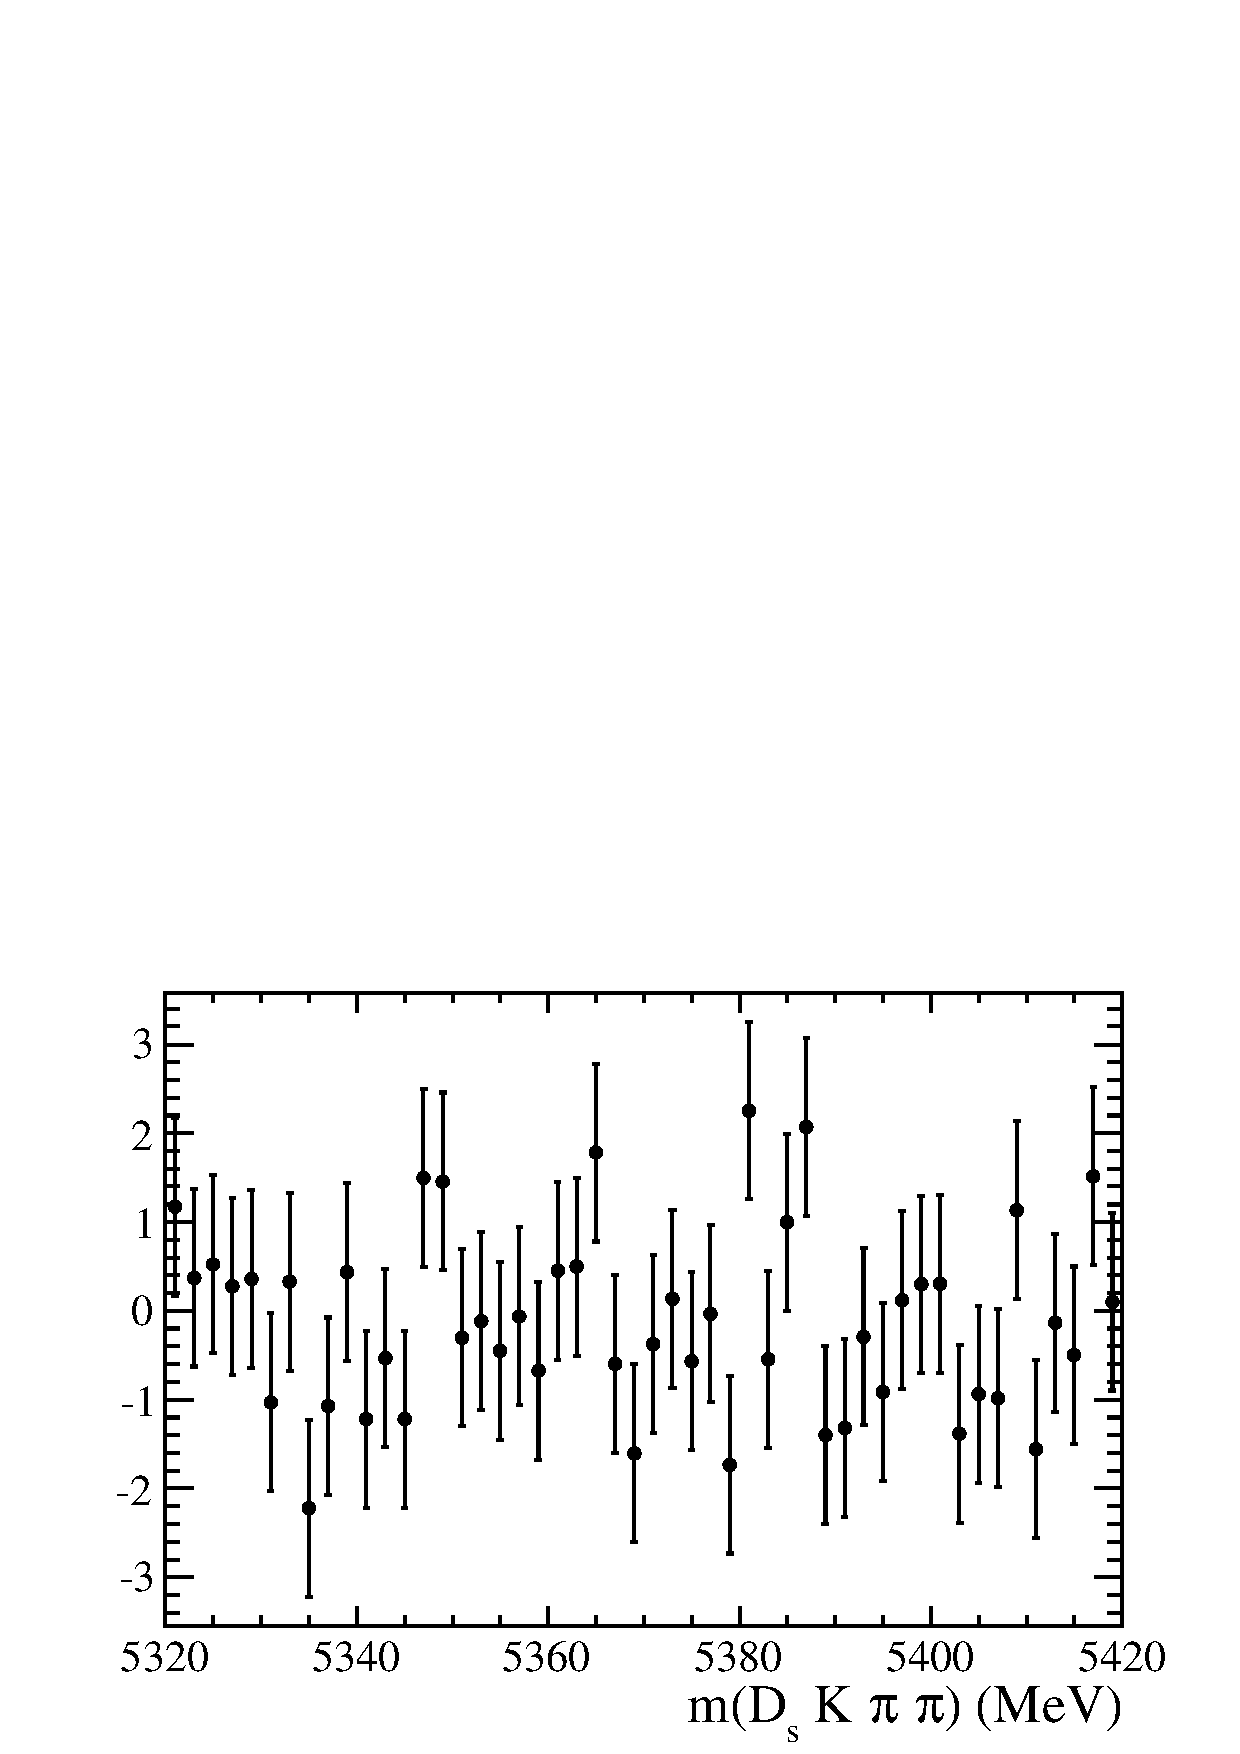
\includegraphics[height=7.cm,width=0.49\textwidth]{figs/MassFit/normMC_pull.pdf}
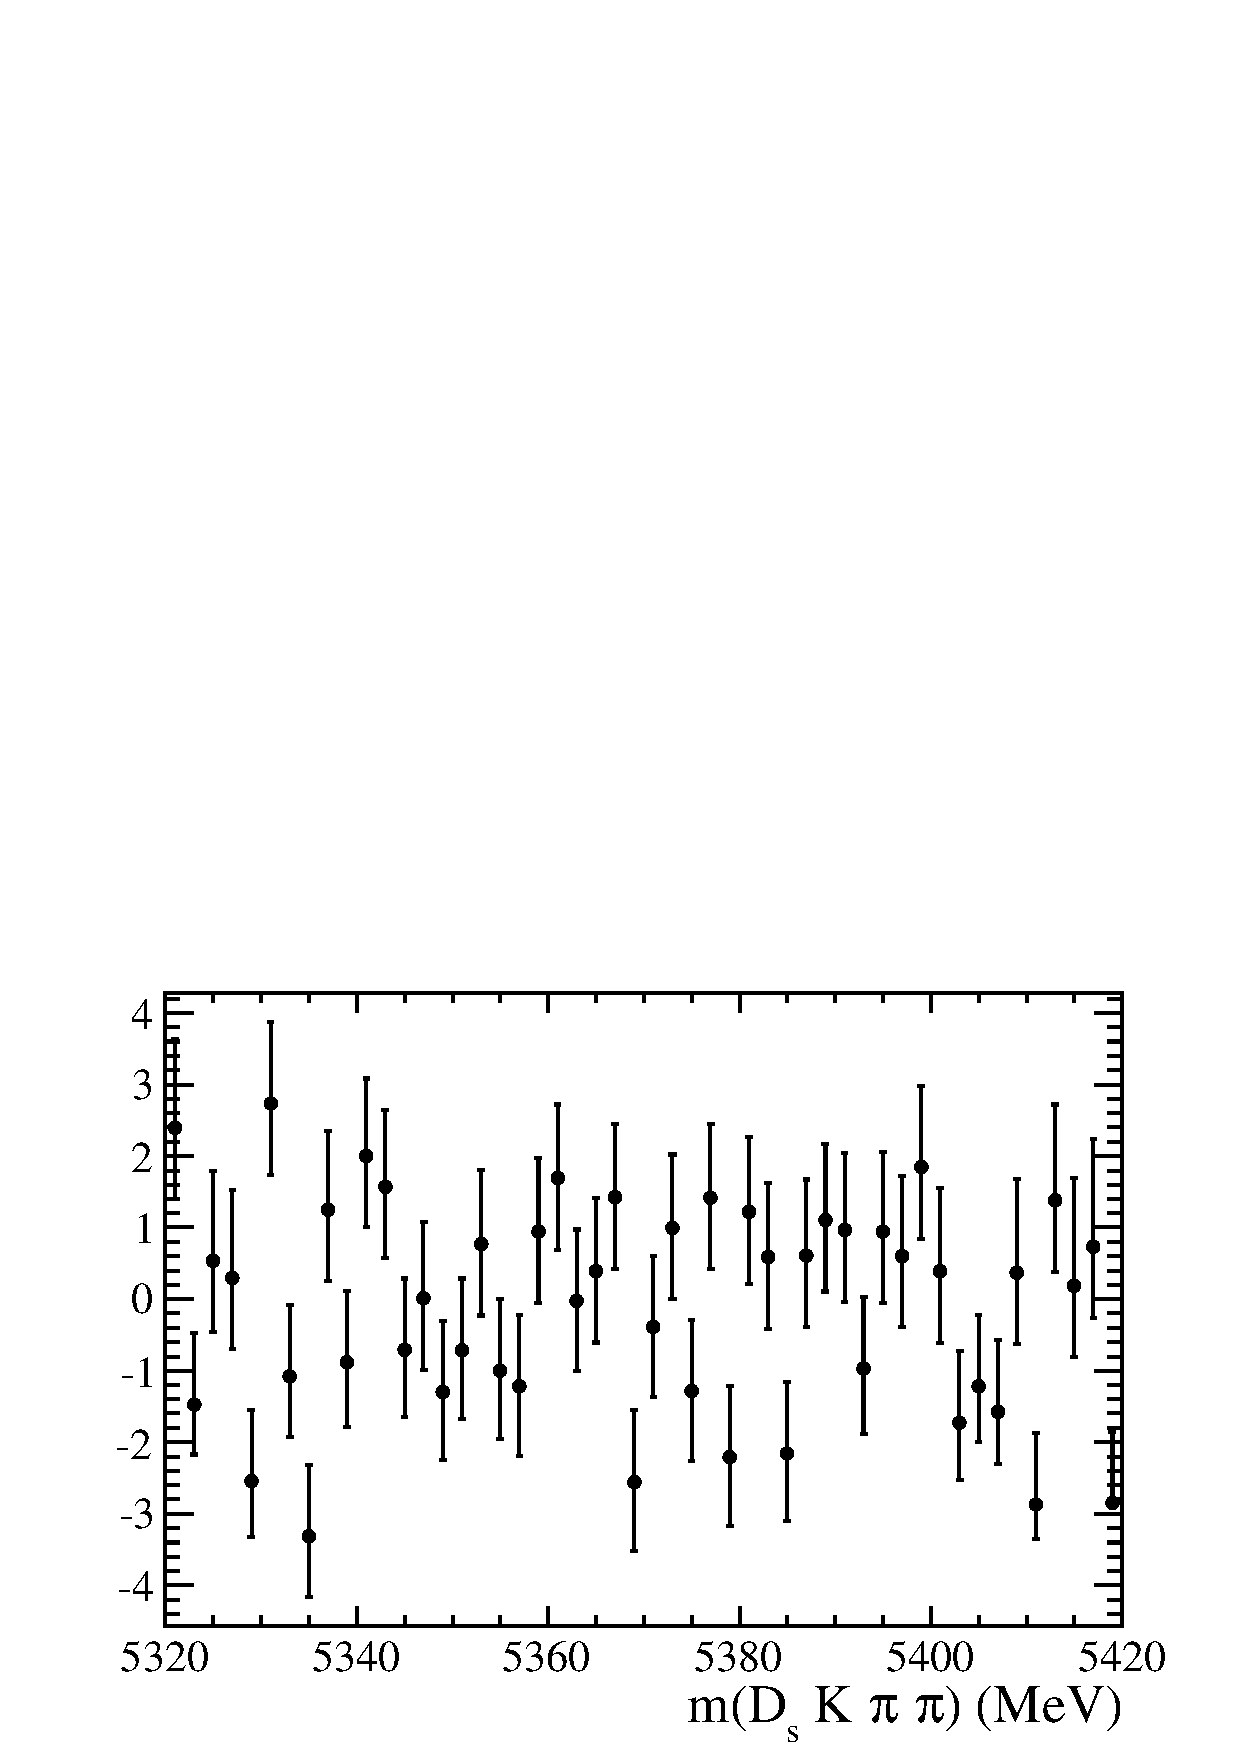
\includegraphics[height=7.cm,width=0.49\textwidth]{figs/MassFit/signalMC_pull.pdf}
\caption{Invariant mass distributions of simulated (left) $\Bs\to\Ds\pion\pion\pion$ and (right) $\Bs\to\Ds\kaon\pion\pion$ events. A fit of a RooJohnsonSU function to each distribution is overlaid.}
\label{fig: BsMassShapes}
\end{figure}

The mass distribution of $\Bs\to\Ds\kaon\pion\pion$ signals is modeled using a Johnson SU function \cite{10.2307/2332539}, which is a gaussian function with a Landau-like tail on one side,

\begin{equation}
J(m_{\Bs};\mu,\sigma,\gamma,\delta) = \frac{\delta}{\sigma 2\pi \sqrt{1+(\frac{m_{\Bs}-\mu}{\sigma})^{2}}} exp \left(-\frac{1}{2}[\gamma + \delta Argsh (\frac{m_{\Bs} - \mu}{\sigma})^{2}]\right).
\label{eq:RooJohnsonSU}
\end{equation}

 
The sign of $\gamma$ in Eq. \ref{eq:RooJohnsonSU} determines whether the tail is located at lower ($\gamma > 0$) or higher ($\gamma < 0$) invariant mass values than the mean $\mu$ of the gaussian function 
and $\delta$ describes the (a)symmetry of the fitted distribution. Higher values of $\delta$ result in a more symmetric, gaussian-like function.    
Another Johnson SU function function is used to account for the contribution of the $\B^{0}\to\Ds\kaon\pion\pion$ decay, which is also present in the $m(\Ds\kaon\pion\pion)$ spectrum.
The width, as well as the tail parameters are fixed to values obtained by a fit to the invariant mass distribution of simulated events shown in Fig \ref{fig: BsMassShapes}. 
A linear scaling factor for the mean $\mu$ and width $\sigma$ is floated in the fit to account for possible differences between the simulation and real data. \newline
The same approach is used to describe the invariant mass distribution of $\Bs\to\Ds\pion\pion\pion$ candidates. 
A  Johnson SU function is used to model the signal, the parameters are determined by a fit to the invariant mass of simulated $\Bs\to\Ds\pion\pion\pion$ decays, shown in Fig \ref{fig: BsMassShapes}.
A scale factor for the width and the mean is floated to account for differences between data and MC.

\subsection{Background models for $\m(\Ds\pion\pion\pion)$} 
\label{subsec: BkginNorm}
Different background sources arise in the invariant mass spectrum of candidates in the normalization mode. \newline
The following backgrounds have to be accounted for:
\begin{itemize}

\item Combinatorial background: This contribution arises from either a real $\Ds$, which is paired with random tracks to form the $\Bs$ candidates, or via real $X_{d}$'s, which are combined with three tracks that fake a $\Ds$ candidate to form a fake $\Bs$.   

\item Partially reconstructed $\Bz/\Bs\to\Ds^{*}\pion\pion\pion$ decays, with $\Ds^{*}\to\Ds\gamma$ or $\Ds^{*}\to\Ds\piz$, where the $\gamma$/$\piz$ is not reconstructed in the decay chain. 

\end{itemize}

In both cases of combinatorial background, the distribution in the invariant mass of $\Bs$ candidates is expected to be smooth and decrease with higher masses. 
Therefore, one exponential function is used to model these contributions. \newline
The shape of the  $\Bs\to\Ds^{*}\pion\pion\pion$ contribution is expected to be peaking in the $m(\Ds\pion\pion\pion)$ spectrum, with large tails due to the missing momentum, which is carried away by the $\piz$ or $\gamma$. 
The pion or photon from $\Ds^{*}\to\Ds(\gamma/\piz)$ is excluded from the reconstruction. 
We model the shape of this contribution using the sum of three bifurcated Gaussian functions.
%\begin{figure}[h]
%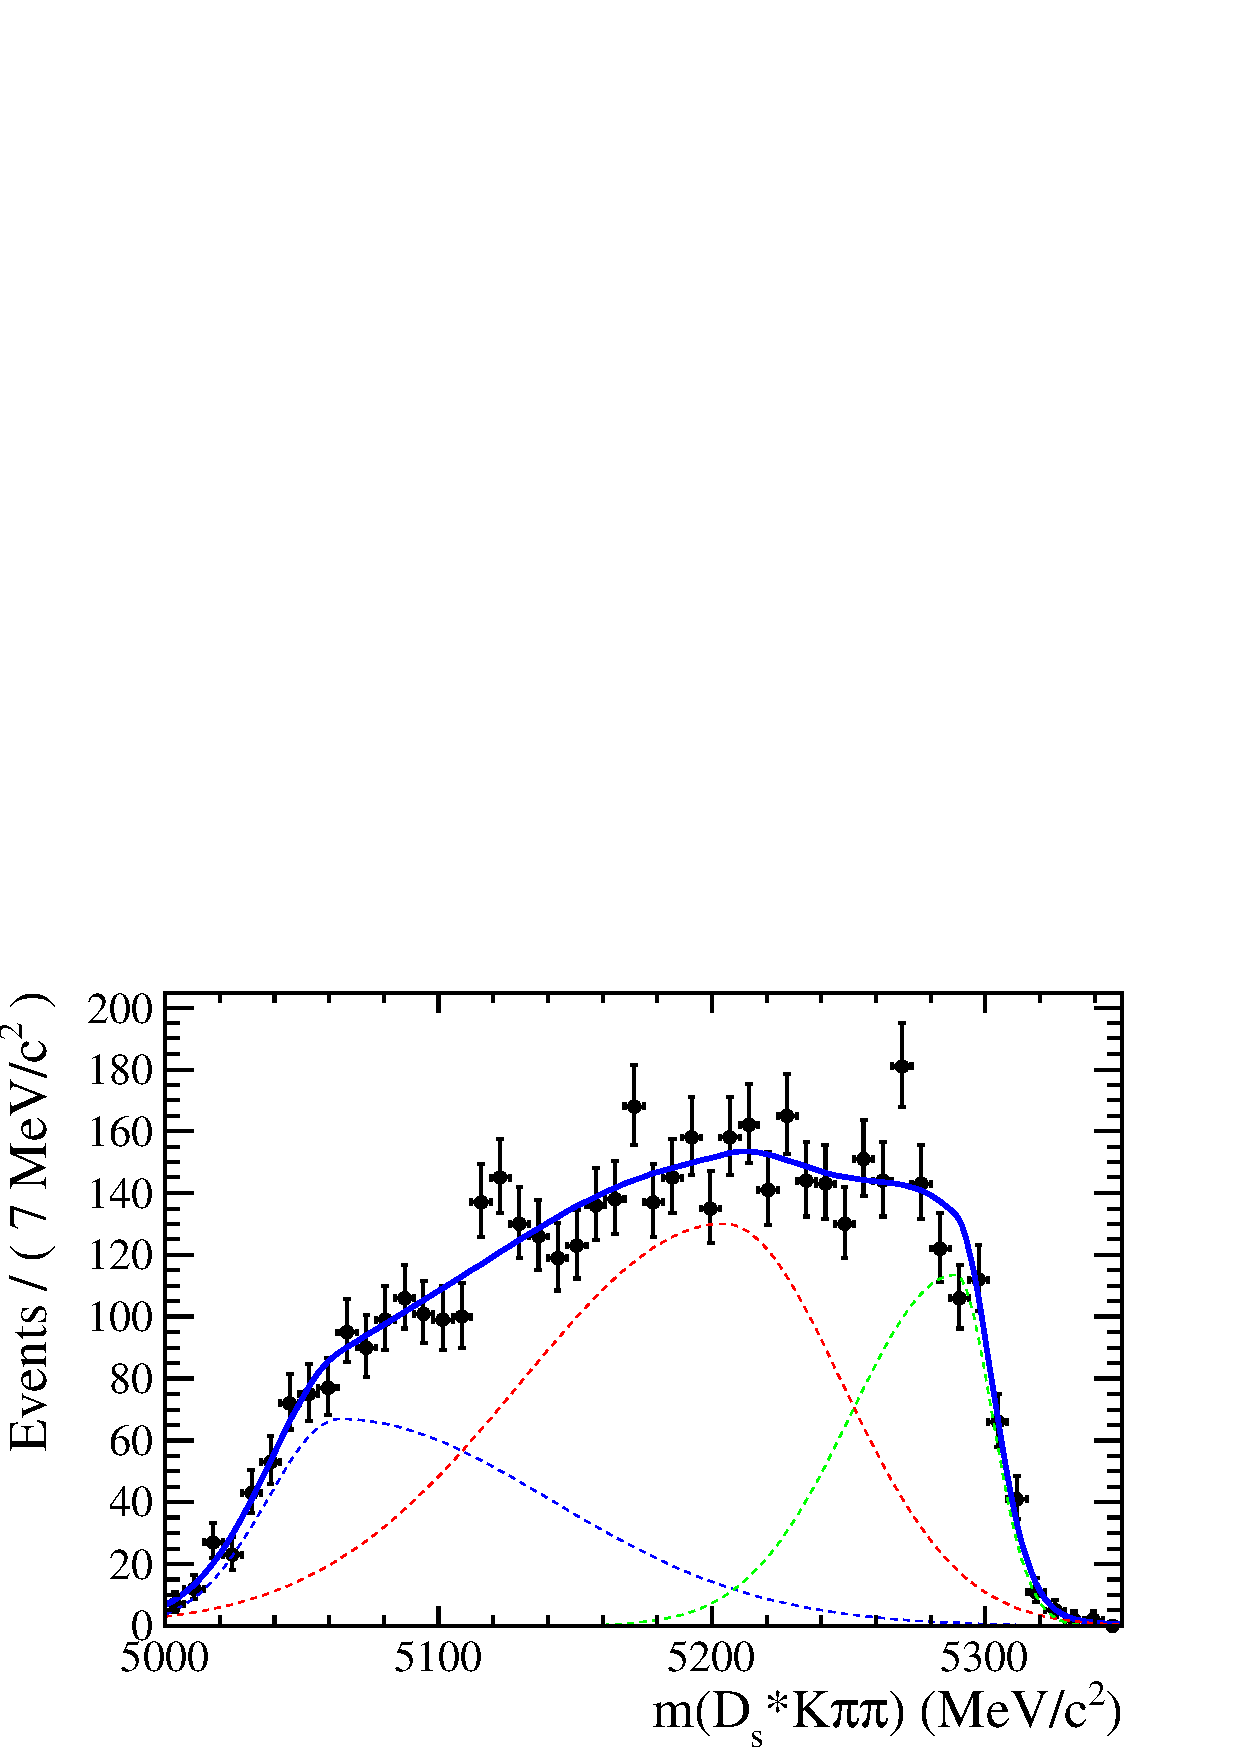
\includegraphics[height=8.cm,width=0.80\textwidth]{figs/Bs2Dsstartpipipi.pdf}
%\caption{Invariant mass distribution of simulated $\Bs\to\Ds^{*}\pion\pion\pion$ events, where the $\gamma$/$\piz$ is excluded from the reconstruction. 
%A fit of the sum of three bifurcated Gaussian functions to this distribution is overlaid.}
%\label{fig: BsDsstar3piMC}
%\end{figure}
%Figure \ref{fig: BsDsstar3piMC} shows the fit of the sum of three bifurcated Gaussian functions to the invariant mass distribution of simulated $\Bs\to\Ds^{*}\pion\pion\pion$ event. 
The shape parameters, 
%are used as input values for the nominal $m(\Ds\pion\pion\pion)$ mass fit. 
as well as the yield of this contribution, are directly determined on data from a fit to the $m(\Ds\pion\pion\pion)$ invariant mass distribution. 

\subsection{Background models for $m(\Ds\kaon\pion\pion)$}
For the signal channel, the following background sources have to be considered:

\begin{itemize}

\item Combinatorial background: same contributions as discussed in Sec. \ref{subsec: BkginNorm}.

\item Partially reconstructed $\Bs\to\Ds^{*}\kaon\pion\pion$ decays, with $\Ds^{*}\to\Ds\gamma$ or $\Ds^{*}\to\Ds\piz$, where the $\gamma$/$\piz$ is not reconstructed in the decay chain. 

\item Partially reconstructed $\Bz\to\Ds^{*}\kaon\pion\pion$ decays, with $\Ds^{*}\to\Ds\gamma$ or $\Ds^{*}\to\Ds\piz$, where the $\gamma$/$\piz$ is not reconstructed in the decay chain.

\item Misidentified $\Bs\to\Ds\pion\pion\pion$ decays, where one of the pions is wrongly identified as a kaon $\pion\rightarrow\kaon$.  

\item Misidentified, partially reconstructed $\Bs\to\Ds^{*}\pion\pion\pion$ decays, where one of the pions is wrongly identified as a kaon $\pion\rightarrow\kaon$ and the $\gamma$/$\piz$ from $\Ds^{*}\to\Ds\gamma$/$\piz$ is 
not reconstructed.

\end{itemize}

The combinatorial background is expected to be non-peaking in the spectrum of the invariant mass of $\Bs\to\Ds\kaon\pion\pion$ candidates. An exponential function is used to model this contribution.\newline
The shape of the partially reconstructed background without misID is taken from our normalization channel, where it can be directly fitted by the sum of three bifurcated Gaussian functions as described above.
In the signal mass fit, all shape parameters for the $\Bs\to\Ds^{*}\kaon\pion\pion$ background are fixed to the input values from our normalization fit.  
%A MC sample of $\Bs\to\Ds^{*}\kaon\pion\pion$ events, where the $\gamma$/$\piz$ is excluded from the reconstruction, is generated. 
%The sum of three bifurcated gaussians is then fitted to the mass distribution of $\Bs$ candidates. The distribution and the overlaid fit is shown in Fig. \ref{fig: BsDsstarKpipiMC}.  

%\begin{figure}[h]
%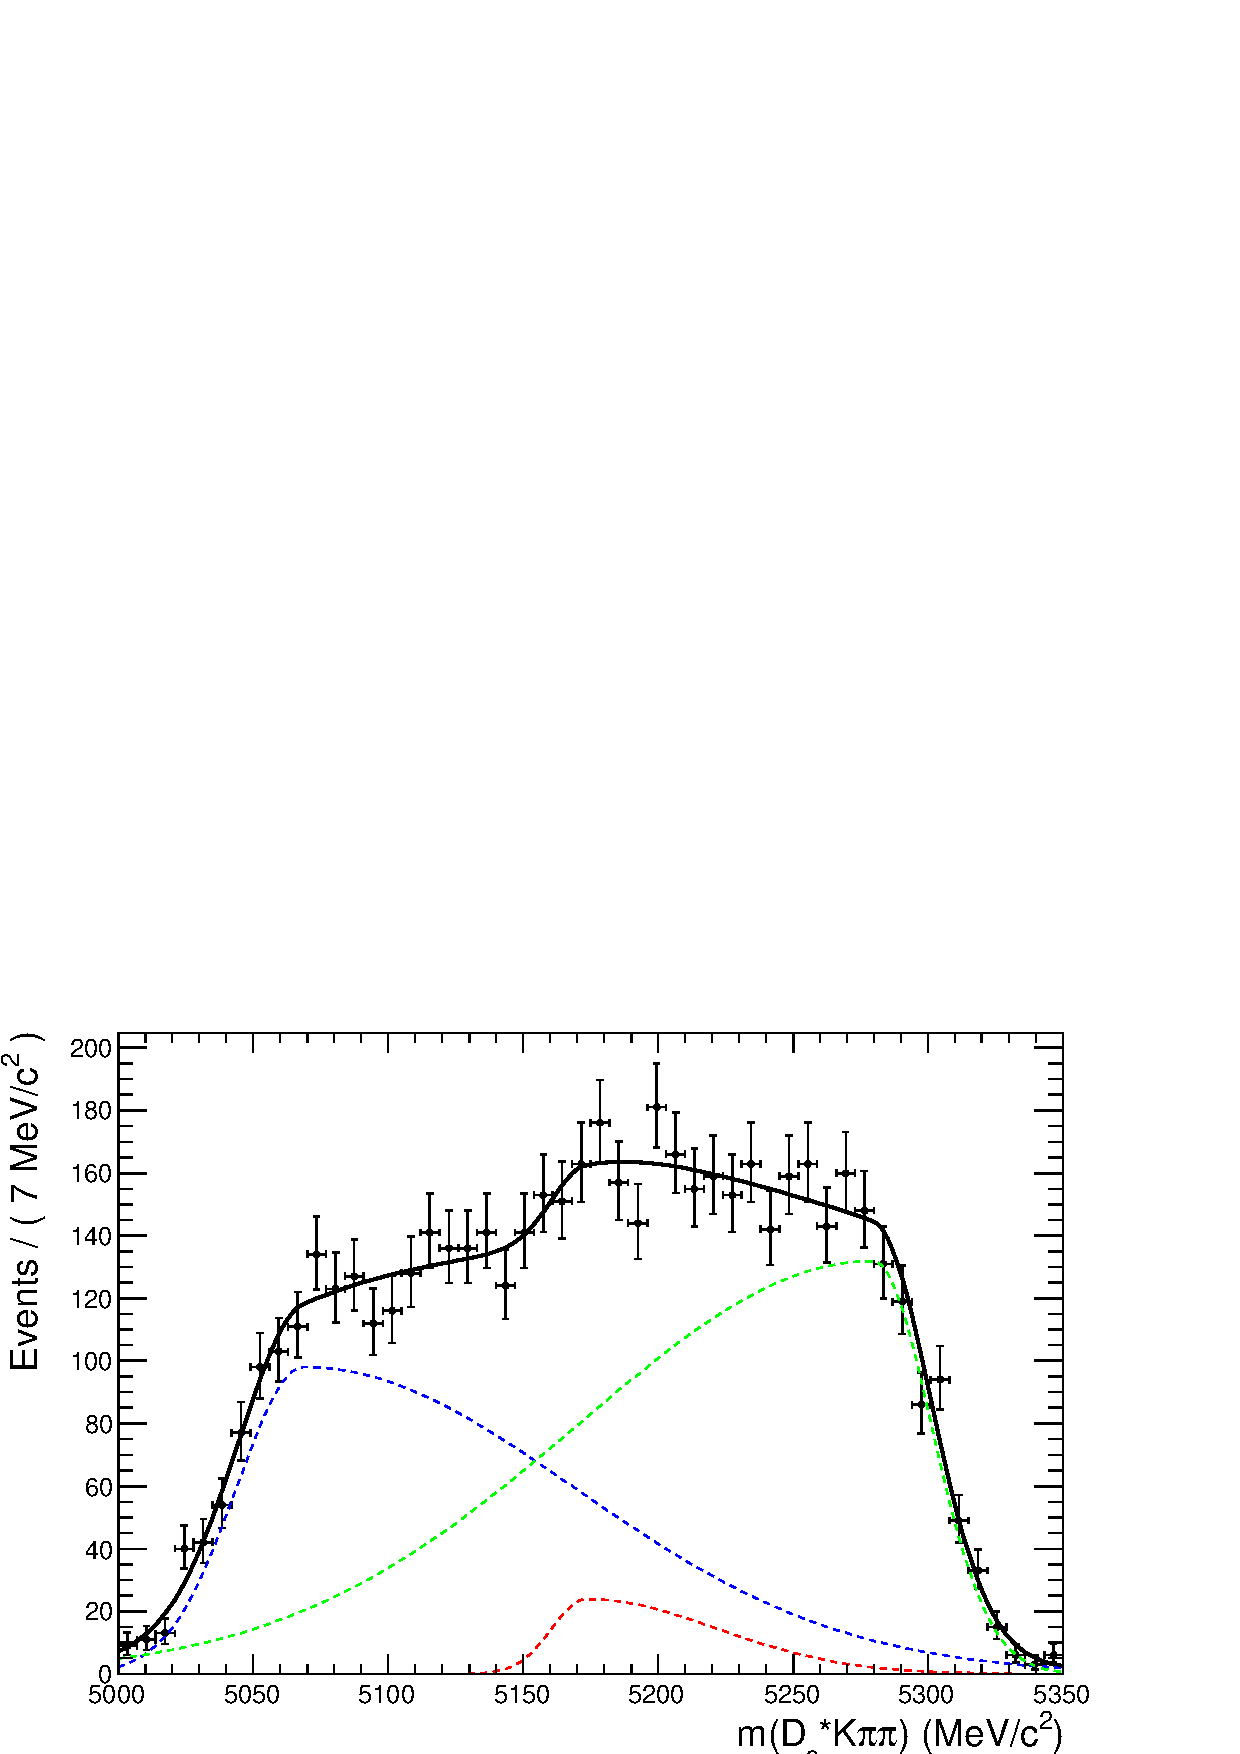
\includegraphics[height=8.cm,width=0.80\textwidth]{figs/Bs2DsstartKpipi.pdf}
%\caption{Invariant mass distribution of simulated $\Bs\to\Ds^{*}\kaon\pion\pion$ events, where the $\gamma$/$\piz$ is excluded from the reconstruction. 
%A fit of the sum of three bifurcated gaussians to this distribution is overlaid.}
%\label{fig: BsDsstarKpipiMC}
%\end{figure}

For the contribution of the $\Bz\to\Ds^{*}\kaon\pion\pion$ background, the same shape is used but the means $\mu_{i}$ of the bifurcated gaussians are shifted down by $m_{\Bs} - m_{\Bz}$ \cite{Agashe:2014kda}. 
The yields of both contributions are directly determined in the nominal fit. \newline
To determine the shape of misidentified $\Bs\to\Ds\pion\pion\pion$ candidates in the $m(\Ds\kaon\pion\pion)$ spectrum, we take a truth-matched signal MC sample of our normalization channel. 
We then use the PIDCalib package to determine the $\pion\rightarrow\kaon$ fake rate. For every candidate in our MC sample, a (momentum) $\ptot$ and (pseudorapidity) $\eta$-dependent event weight is computed and assigned. 
We flip the particle hypothesis from pion to kaon for the $\pion$ with the biggest miss-ID weight for each event and recompute the invariant $\Bs$ mass. This distribution is then modeled using two Crystal Ball functions. 
The distribution and the fit are shown in Fig. \ref{fig: BsDspipipiMCmissID}(left). 

\begin{figure}[h]
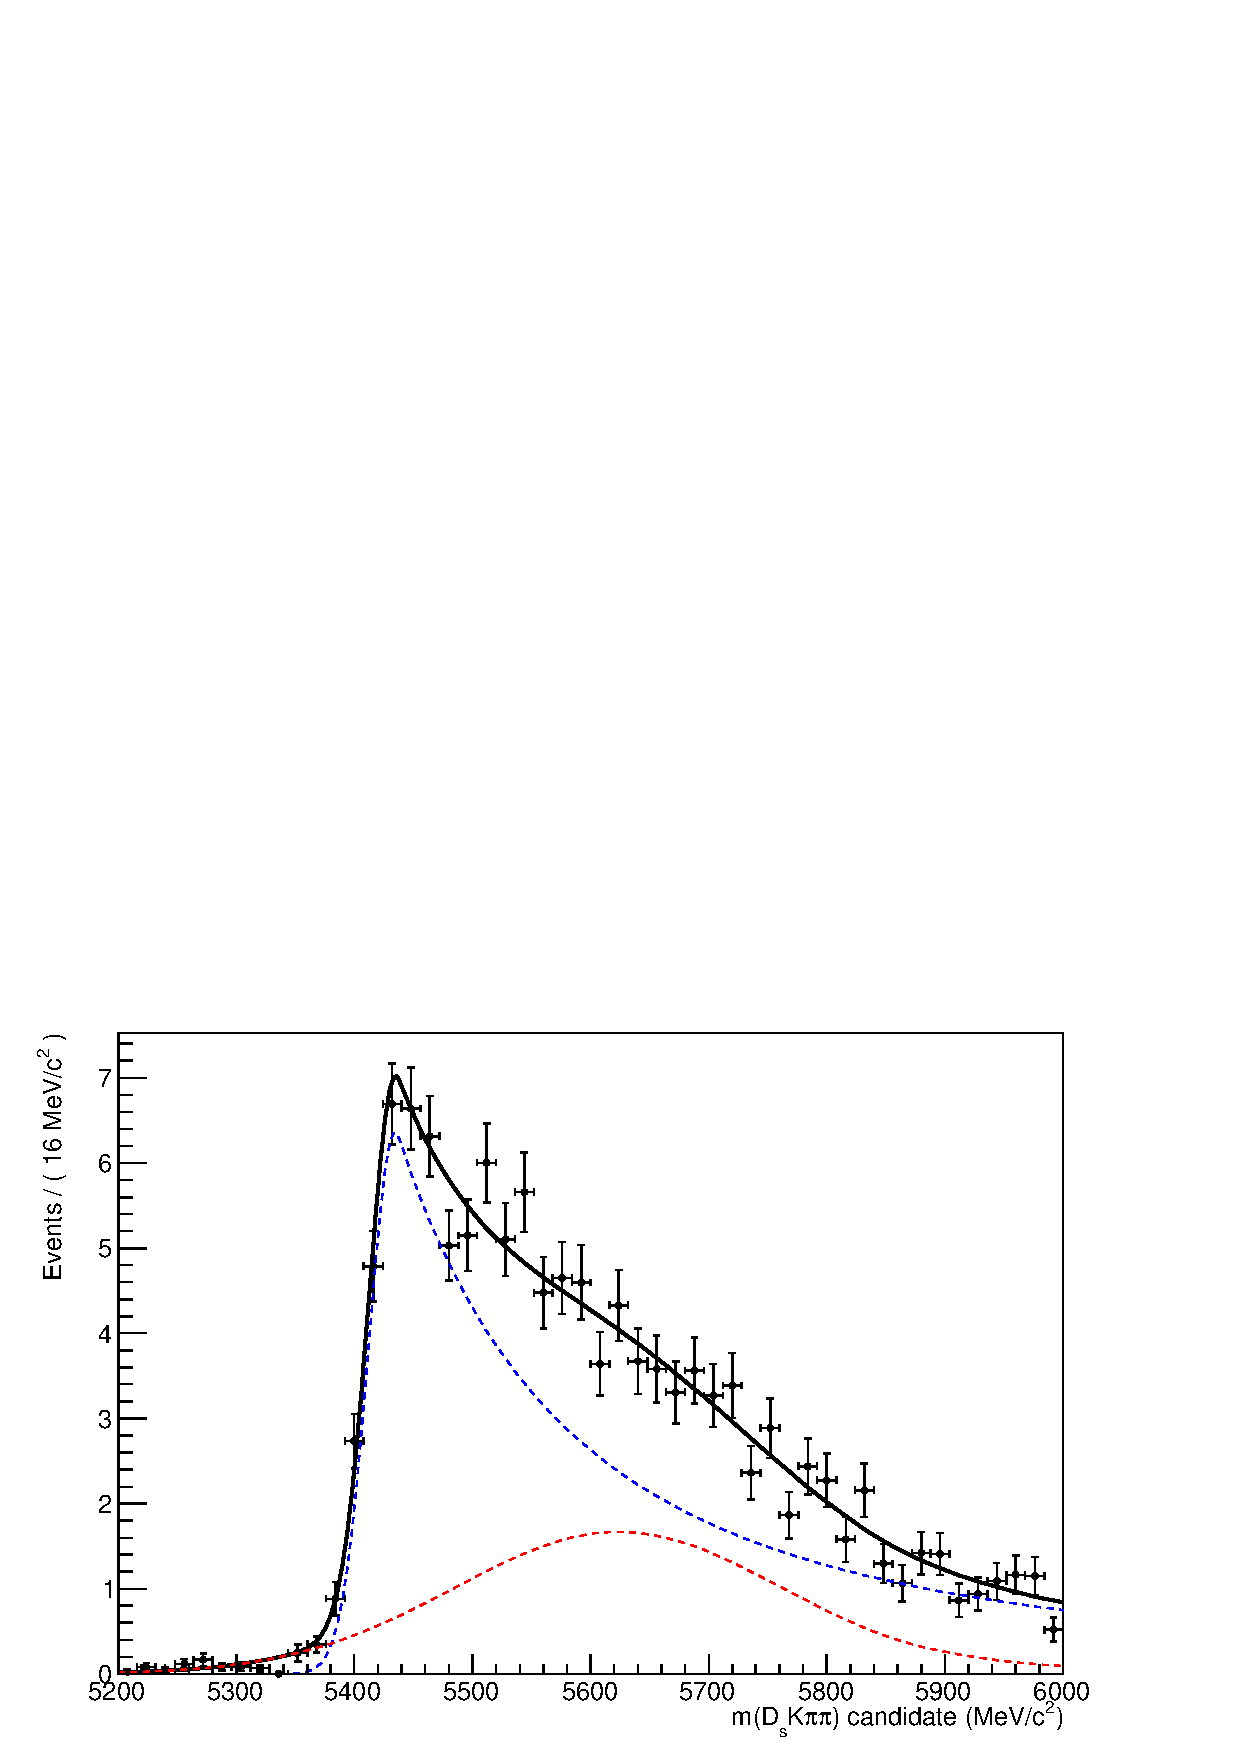
\includegraphics[height=6.cm,width=0.45\textwidth]{figs/Bs2Dspipipi_as_DsKpipi.pdf}
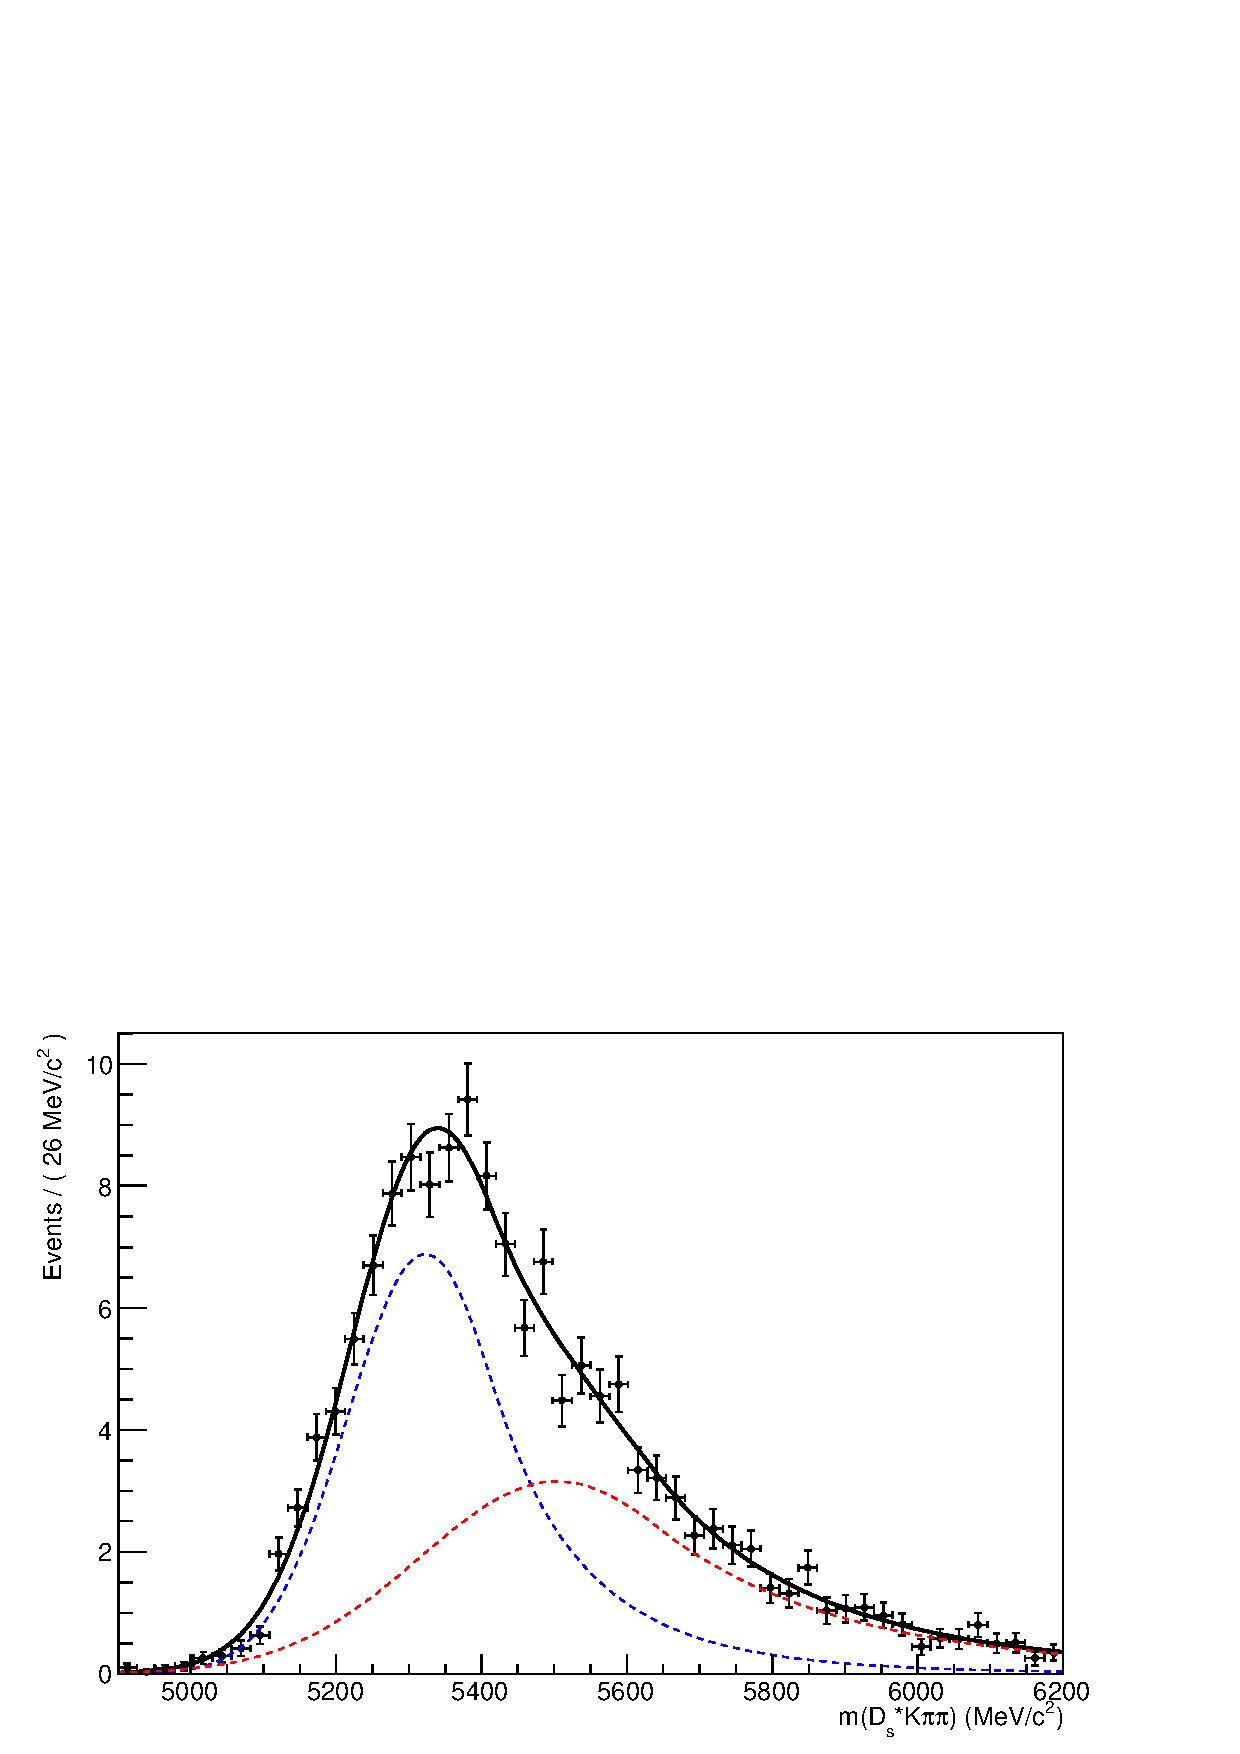
\includegraphics[height=6.cm,width=0.45\textwidth]{figs/Bs2Dsstarpipipi_as_DsKpipi.pdf}
\caption{Invariant mass distribution of (left) simulated $\Bs\to\Ds\pion\pion\pion$ events, where one of the $\pion$'s is reconstructed as a $\kaon$ and the misID probability for each event is taken into account. 
The corresponding distribution for simulated $\Bs\to\Ds^{*}\pion\pion\pion$ events, where the $\gamma$/$\piz$ from the $\Ds^{*}$ is excluded from reconstruction, is shown on the right.
The solid, black curve on each plot corresponds to the fit consisting of two Crystal Ball functions.}
\label{fig: BsDspipipiMCmissID}
\end{figure}
 
The expected yield of misidentified $\Bs\to\Ds\pion\pion\pion$ candidates in the $m(\Ds\kaon\pion\pion)$ spectrum is computed by multiplying the fake probability of $\propto3.2\%$, which is derived from PIDCalib, by the yield of $\Bs\to\Ds\pion\pion\pion$ signal candidates, determined in the nominal mass fit of our normalization channel.  \newline
In the same way as mentioned above, we can determine the rate of misidentified, partially reconstructed $\Bs\to\Ds^{*}\pion\pion\pion$ decays in our sample of $\Bs\to\Ds\kaon\pion\pion$ decays using PIDCalib and a MC sample of $\Bs\to\Ds^{*}\pion\pion\pion$ events. The invariant mass distribution we obtain when we exclude the $\gamma$/$\piz$, flip the the particle hypothesis $\pion\rightarrow\kaon$ and apply the event weights given by the fake rate, is shown in Fig. \ref{fig: BsDspipipiMCmissID} (right). The fit of two Crystal Ball functions to this distribution is overlaid. 
The yield of this contribution is determined from the yield of $\Bs\to\Ds^{*}\pion\pion\pion$ candidates in the nominal mass fit of our normalization channel, multiplied by the misID probability of $\propto 3.6\%$.
 



\subsection{Fit to $\Bs\to\Ds\pion\pion\pion$ candidates}
\label{subsec: NormFit}

An unbinned maximum likelihood fit is performed simultaneously to the invariant mass distribution of $\Bs\to\Ds\pion\pion\pion$ candidates. 
As discussed in Sec. \ref{subsec: signalmodel}, the fit is given as a Johnson SU signal model for the $\Bs$ and $\Bz$ signal, the sum of three bifurcated Gaussian functions to model the partially reconstructed $\Bs\to\Ds^{*}\pion\pion\pion$ background and an Exponential function to account for combinatorial background. The invariant mass distribution and the fit is shown in Fig. \ref{fig: BsDsKpipiFit}. 
All simultaneously performed fits to the $m(\Ds\pion\pion\pion)$ distribution, ordered by the respective $\Ds$ final state, can be found in the Appendix \ref{subsec:DetailedMassfits}.   
The obtained yields are summarized in Table \ref{table:YieldsFromMassfit}. 


\subsection{Fit to $\Bs\to\Ds\kaon\pion\pion$ candidates}
\label{subsec: SigFit}

The shape of the invariant mass distribution of$\Bs\to\Ds\kaon\pion\pion$ candidates is described by Johnson SU functions for the $\Bz$ and $\Bs$ signal, 
two sums of three bifurcated Gaussians for the $\Bs$/$\Bz\to\Ds^{*}\kaon\pion\pion$ partially reconstructed background contributions and 
two sums of double Crystal Ball functions for the single misID $\Bs\to\Ds\pion\pion\pion$ and the partially reconstructed, misidentified $\Bs\to\Ds^{*}\pion\pion\pion$ decays. 
A simultaneous unbinned maximum likelihood fit is performed and the result is shown in Fig. \ref{fig: BsDsKpipiFit}.
All simultaneously performed fits to the $m(\Ds\kaon\pion\pion)$ distribution, ordered by the respective $\Ds$ final state, can be found in the Appendix \ref{subsec:DetailedMassfits}.
The obtained yields are summarized in Table \ref{table:YieldsFromMassfit}.
 

\subsection{Extraction of signal weights}
\label{subsec: sWegihts}

The sPlot technique \cite{Pivk:2004ty} is used to extract signal weights from the fits to the invariant mass distributions of our signal and normalizaton channel. 
This statistical tool assignes a weight to every event, according to it's position in the respective mass distribution, given the fitted signal and background models. 
The weights can then be used to suppress the background components in every other observable distribution of interest.  
Figure \ref{fig: sWeights} shows the distribution of weights across the invariant mass spectra of $\Bs\to\Ds\pion\pion\pion$ and $\Bs\to\Ds\kaon\pion\pion$ candidates.


\begin{figure}[h]
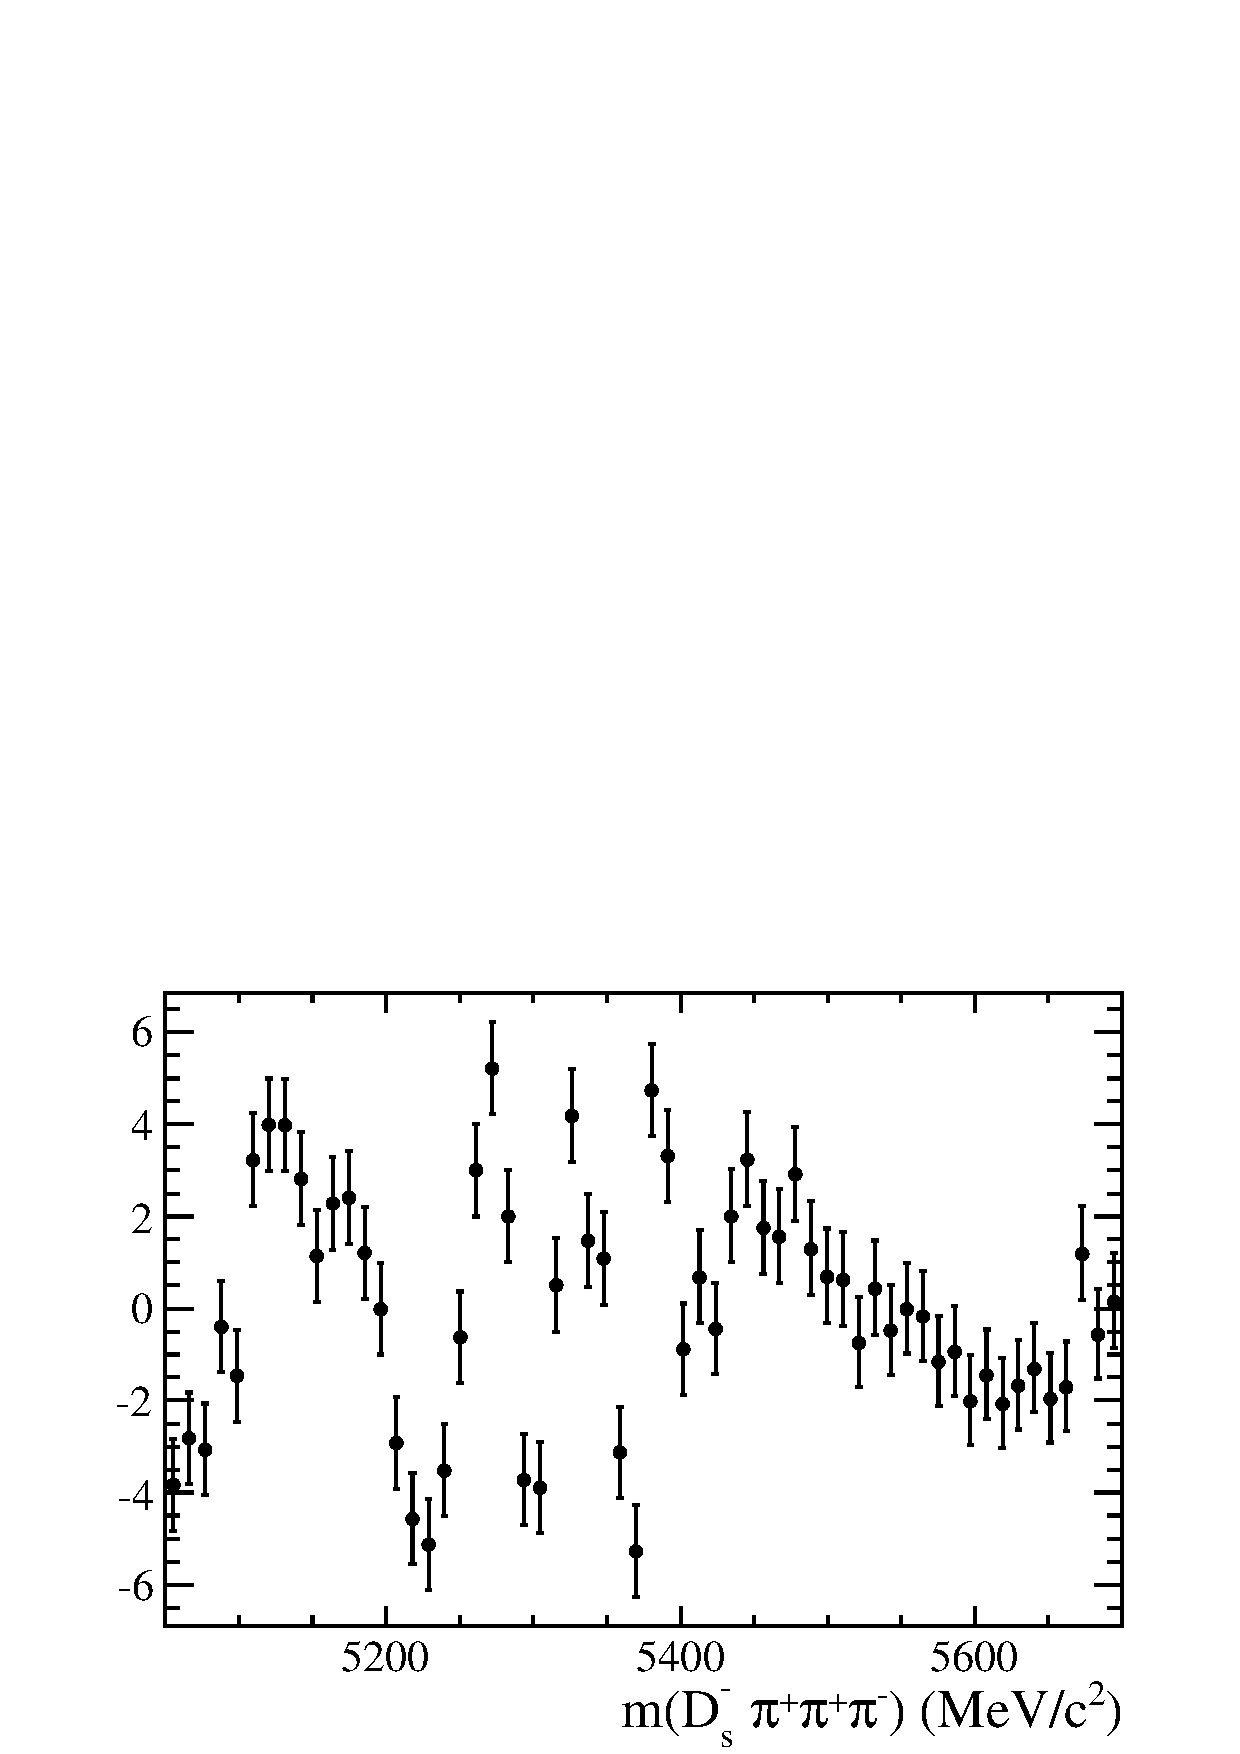
\includegraphics[height=7.cm,width=0.49\textwidth]{figs/MassFit/norm_pull.pdf}
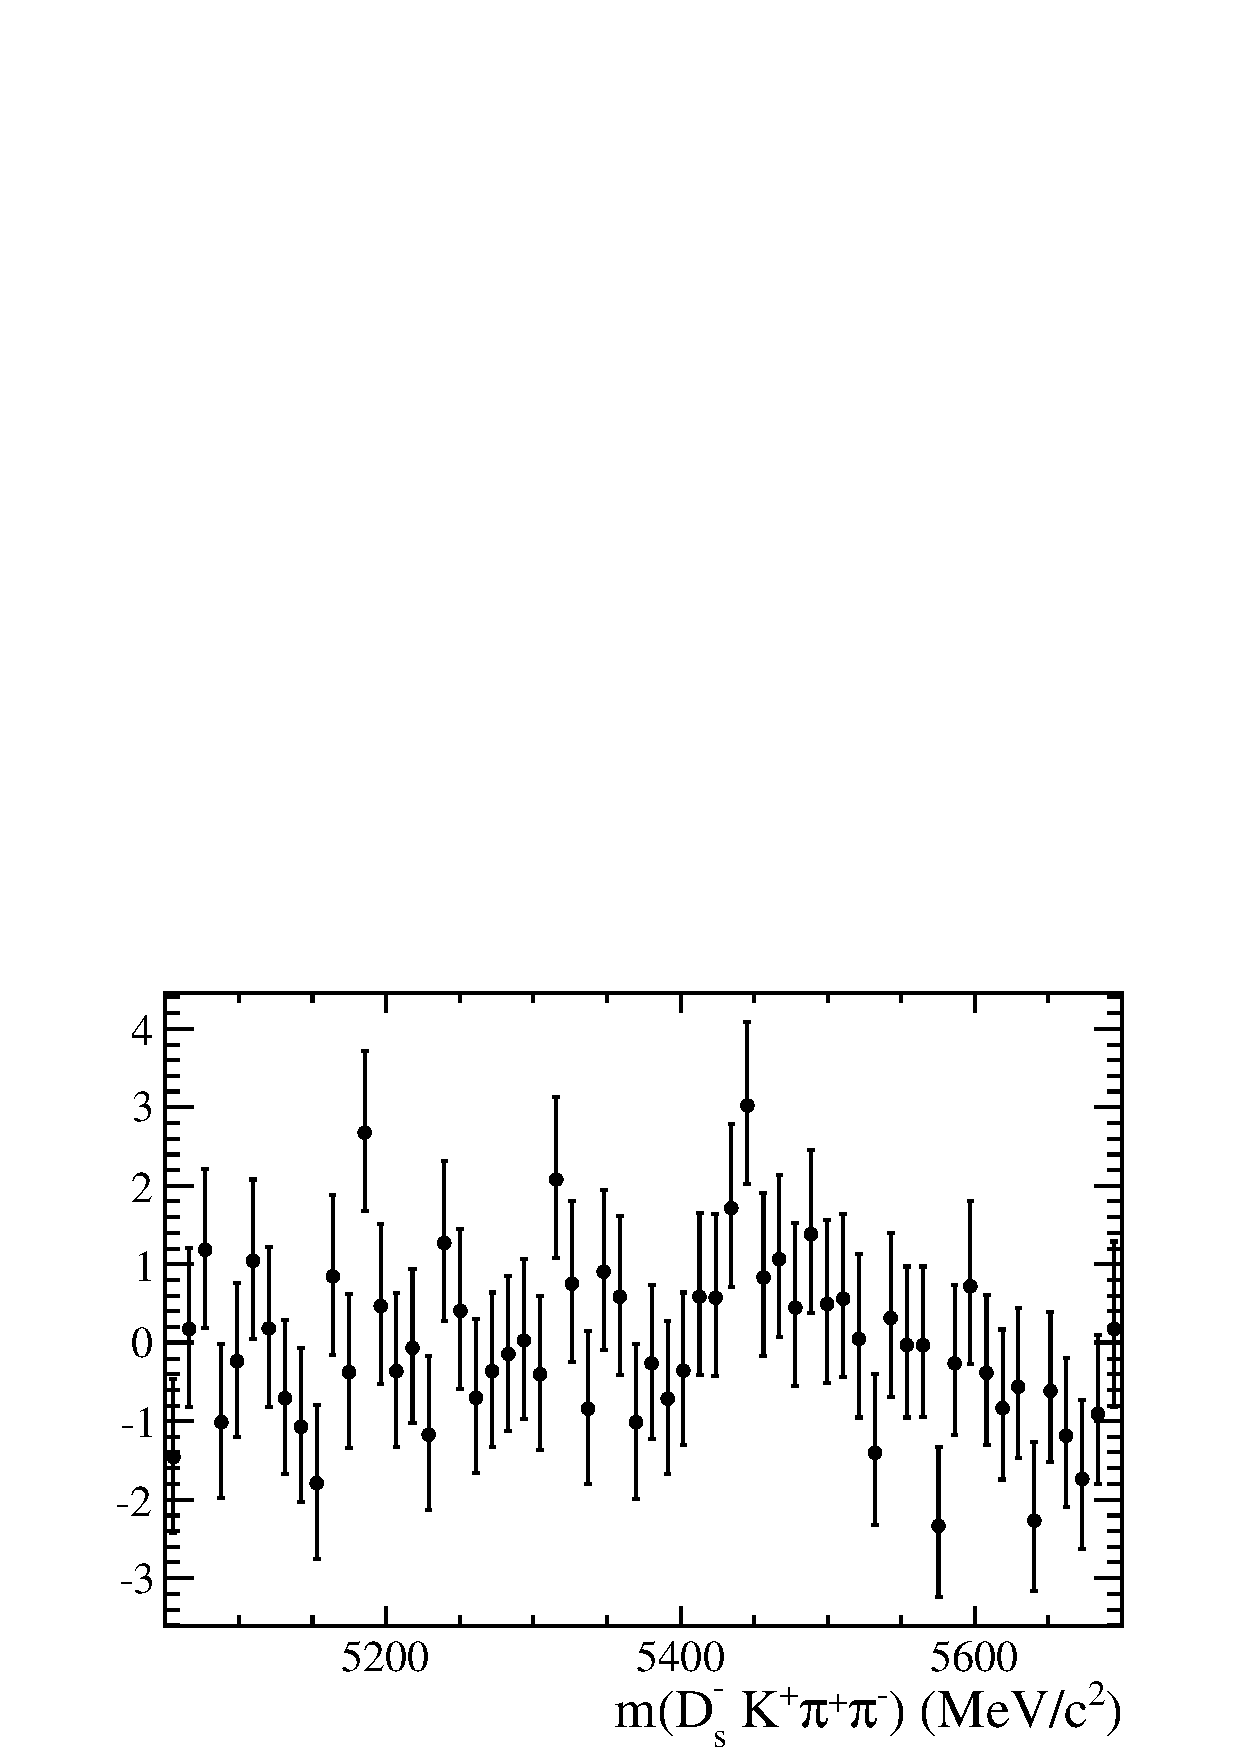
\includegraphics[height=7.cm,width=0.49\textwidth]{figs/MassFit/signal_pull.pdf}
\caption{Invariant mass distribution of (left) $\Bs\to\Ds\pion\pion\pion$ and (right) $\Bs\to\Ds\kaon\pion\pion$ candidates for Run1 and Run2 data.
The respective fit described in the text is overlaid.}
\label{fig: BsDsKpipiFit}
\end{figure}


\begin{table}[h]
\centering
 \begin{tabular}{l || l l l l}
fit component & yield 2011 & yield 2012 & yield 2015 & yield 2016\ \\
\hline\hline
$m(\Ds\kaon\pion\pion)$ &  &  &  &  \\
\hline
$\Bs\to\Ds\kaon\pion\pion$ & 392 $\pm$ 25 & 860 $\pm$ 38 & 309 $\pm$ 21 & 1984 $\pm$ 55 \\
$\Bz\to\Ds\kaon\pion\pion$ & 276 $\pm$ 26 & 692 $\pm$ 41 & 261 $\pm$ 23 & 1385 $\pm$ 58 \\
$\Bz/\Bs\to\Ds^{*}\kaon\pion\pion$ & 7 $\pm$ 25 & 171 $\pm$ 75 & 114 $\pm$ 25 & 893 $\pm$ 84 \\
$\Bs\to\Ds^{(*)}\pion\pion\pion$ & 63 $\pm$ 0 & 158 $\pm$ 0 & 53 $\pm$ 0 & 314 $\pm$ 0 \\
combinatorial & 1482 $\pm$ 53 & 2884 $\pm$ 100 & 605 $\pm$ 43 & 4261 $\pm$ 133 \\
\hline\hline
$m(\Ds\pion\pion\pion)$ &  &  &  &  \\
\hline
$\Bs\to\Ds\pion\pion\pion$ & 9183 $\pm$ 105 & 22083 $\pm$ 166 & 7574 $\pm$ 95 & 43773 $\pm$ 245 \\
$\Bz\to\Ds\pion\pion\pion$ & 289 $\pm$ 58 & 716 $\pm$ 95 & 229 $\pm$ 54 & 968 $\pm$ 147 \\
$\Bs\to\Ds^{*}\pion\pion\pion$ & 3640 $\pm$ 130 & 9086 $\pm$ 232 & 3047 $\pm$ 110 & 17827 $\pm$ 421 \\
combinatorial & 4991 $\pm$ 154 & 11127 $\pm$ 271 & 3728 $\pm$ 126 & 24589 $\pm$ 500 \\
\hline
\end{tabular}
\caption{Summary of yields obtained from the fits to Run1 and Run2 data.}
\label{table:YieldsFromMassfit}
\end{table}


%\begin{figure}[h]
%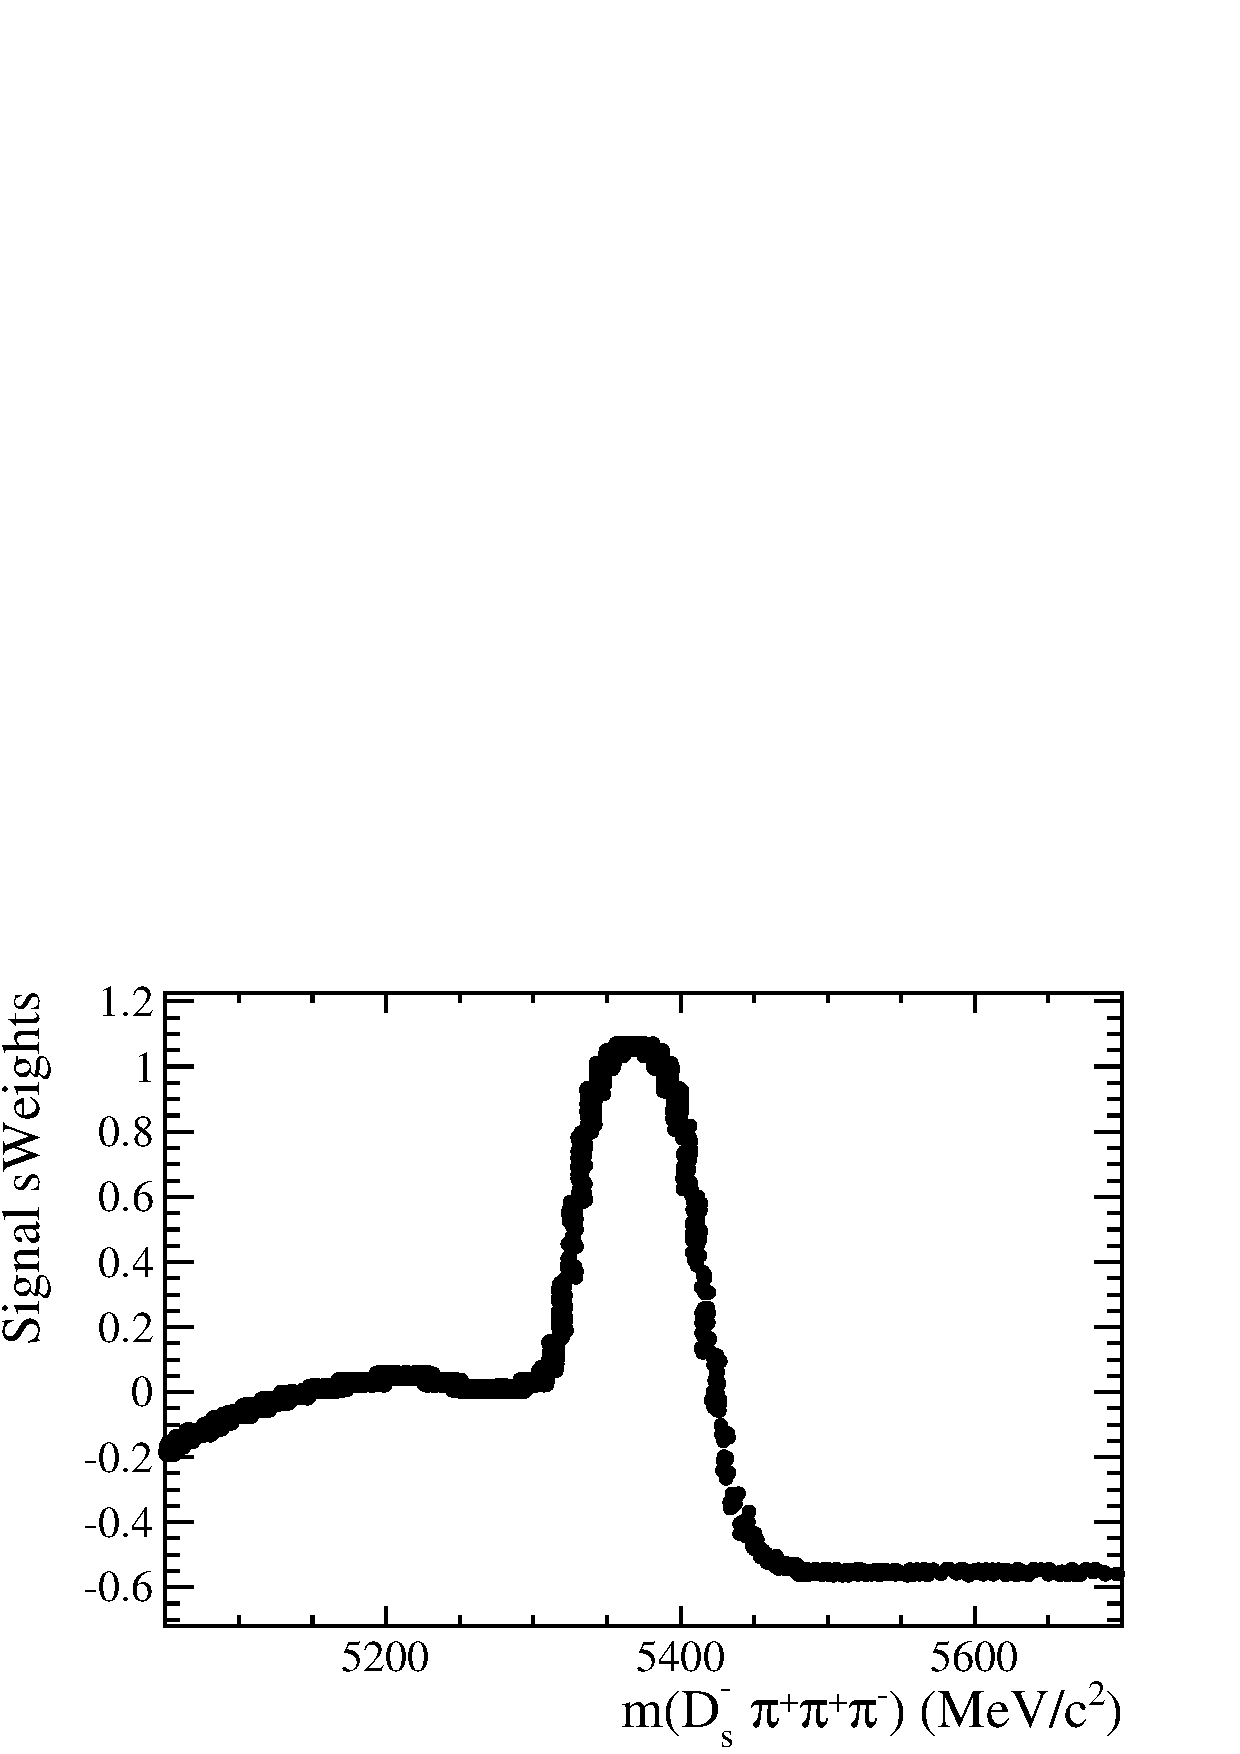
\includegraphics[height=7.cm,width=0.49\textwidth]{figs/norm_sweight_y11_phipi.pdf}
%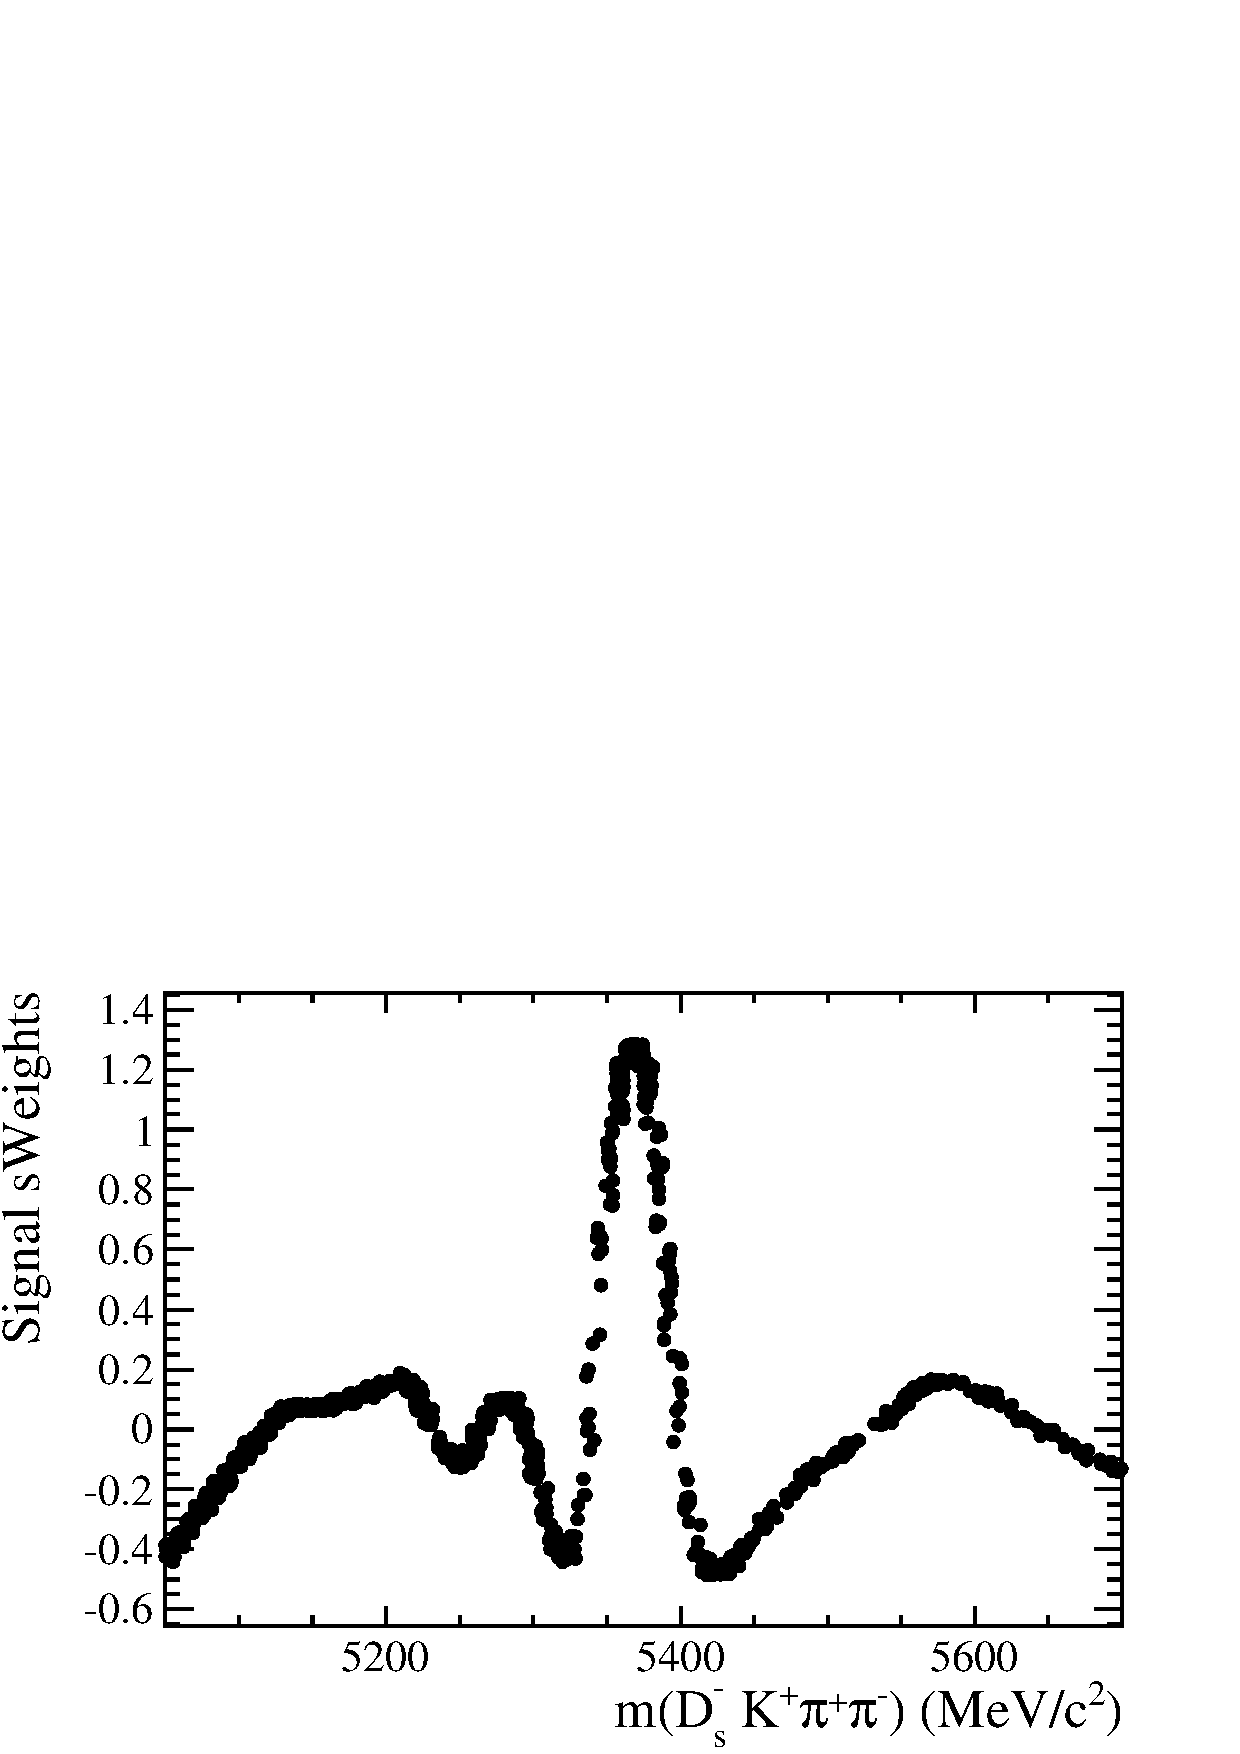
\includegraphics[height=7.cm,width=0.49\textwidth]{figs/signal_sweight_y11_phipi.pdf}
%\caption{Distribution of sWeights across the invariant mass of (left) $\Bs\to\Ds\pion\pion\pion$ and (right) $\Bs\to\Ds\kaon\pion\pion$ candidates for Run1 and Run2 data.}
%\label{fig: sWeights}
%\end{figure}


\clearpage
% !TEX root = main.tex

\section{Decay-time Resoution}
\label{sec:Resolution}

The observed oscillation of B mesons is prone to dilution, if the detector resolution is of similar magnitude as the oscillation period. 
In the \Bs system, considering that the measured oscillation frequency of the \Bs \cite{PDG2014} and the average LHCb detector resolution \cite{LHCb-DP-2014-002} are both $\mathcal{O}(50 \fs^{-1})$, this is the case.
Therefore, it is crucial to correctly describe the decay time resolution in order to avoid a bias on the measurement of time dependent CP parameters. \newline
In the presented analysis, we assume a gaussian resolution function with different widths for each event. 
This gives rise to a per-event decay time error $\sigma_{t}$, which is computed separately for every event along with the proper time $t$, by the decay time fitter. 
Furthermore, the per-event decay time error $\sigma_{t}$ is usualy underestimated by the decay time fitter, 
making it necessary to derive a scaling function, which matches the per-event error to the actually measured decay time resolution. 
In the following, we investigate the Run1 and Run2 MC samples to find the proper decay time resolution in bins of the per-event decay time erros and derive a scaling function from that.      


\subsection{Formalism}

Describtion here ...




\subsection{Results}

Summary of results and MC/Data correction from $\Ds\kaon$ here ...


\begin{figure}[h]
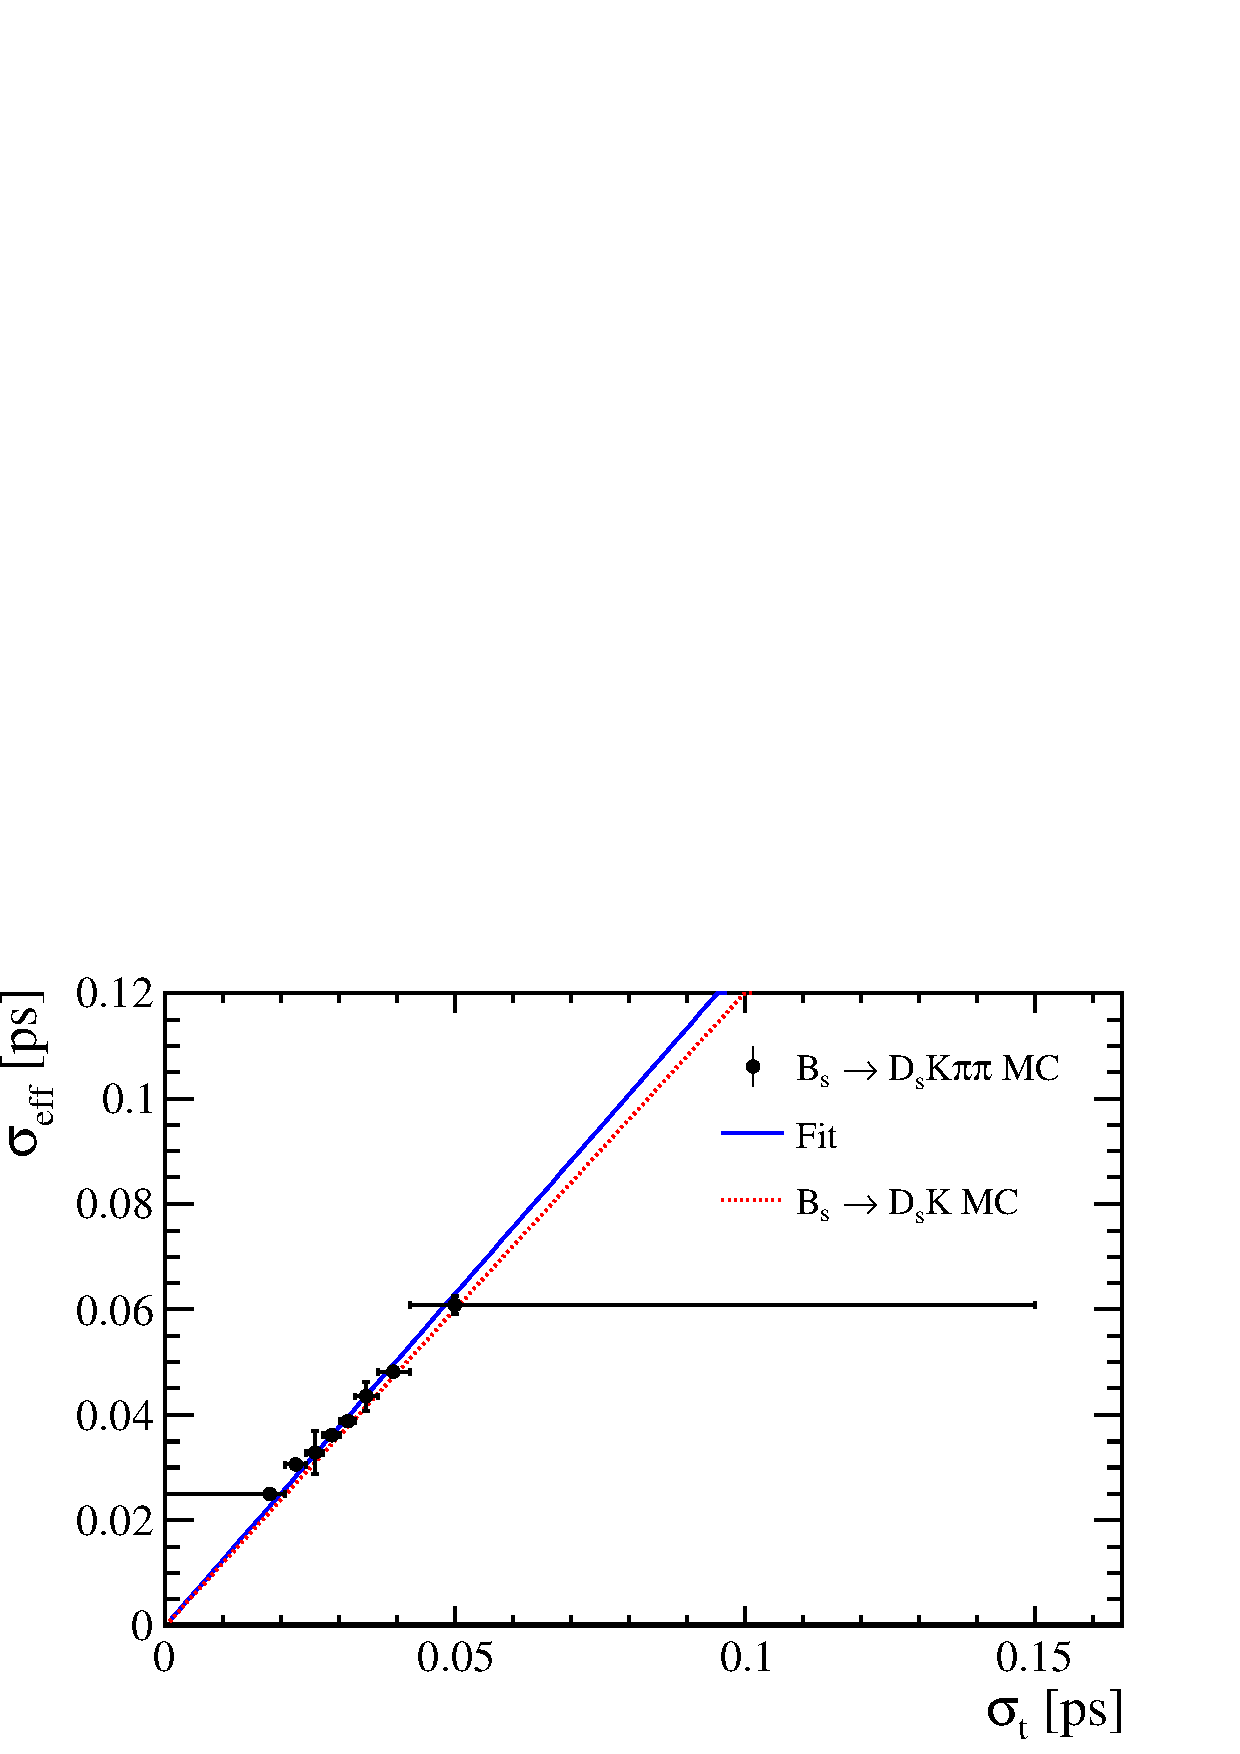
\includegraphics[height=7.4cm,width=0.7\textwidth]{figs/ProperTimeReso_MC.pdf}
\caption{Decay-time resolution of $\Bs\to\Ds\kaon\pion\pion$ candidates from MC. The fit described in the text is overlaid.}
\label{fig:ResoFit_compared}
\end{figure}


\begin{table}[h]
\centering
 \begin{tabular}{l || l l l | l l}
$\sigma_{t}$ Bin [fs] & $\sigma_{1}$ [fs] & $\sigma_{2}$ [fs] & $f_{1}$ & D & $\sigma_{eff}$ [fs] \\
\hline
0to19 & 22.57 $\pm$ 0.96 & 45.57 $\pm$ 4.061 & 0.827 $\pm$ 0.057 & 0.89 $\pm$ 0.067 & 27.46 $\pm$ 8.82 \\
19to24 & 24.64 $\pm$ 1.03 & 46.65 $\pm$ 3.109 & 0.768 $\pm$ 0.061 & 0.86 $\pm$ 0.070 & 30.64 $\pm$ 8.48 \\
24to29 & 30.96 $\pm$ 0.90 & 58.76 $\pm$ 5.684 & 0.884 $\pm$ 0.045 & 0.83 $\pm$ 0.05 & 34.66 $\pm$ 5.28 \\
29to34 & 35.28 $\pm$ 1.54 & 57 $\pm$ 6.698 & 0.839 $\pm$ 0.098 & 0.79 $\pm$ 0.10 & 39.09 $\pm$ 10.47 \\
34to39 & 37.05 $\pm$ 2.36 & 61.98 $\pm$ 5.769 & 0.707 $\pm$ 0.12 & 0.73 $\pm$ 0.12 & 44.76 $\pm$ 11.78 \\
39to44 & 68.38 $\pm$ 8.33 & 42.15 $\pm$ 3.583 & 0.331 $\pm$ 0.18 & 0.66 $\pm$ 0.16 & 50.98 $\pm$ 15.11 \\
44to49 & 199.9 $\pm$ 100.1 & 53.72 $\pm$ 1.419 & 0.020 $\pm$ 0.014 & 0.62 $\pm$ 0.02 & 54.89 $\pm$ 1.60 \\
49to150 & 68.75 $\pm$ 165.3 & 68.92 $\pm$ 4.603 & 0.001 $\pm$ 0.97 & 0.47 $\pm$ 0.65 & 68.92 $\pm$ 63.42 \\
\hline
\end{tabular}
\caption{Summary of the obtained parameters from the resolution fits described above.}
\label{table:ResoParams}
\end{table}



\clearpage
\section{Decay-time acceptance}
\label{sec:Acceptance}

The decay-time distribution of the $\Bs$ mesons is distorted due to the geometry of the LHCb detector and the applied selections, described in Section \ref{sec:Selection}.
In particular, any requirement on the flight distance, the impact parameter or the direction angle (DIRA) of the $\Bs$ mesons leads to a decay-time dependent efficiency $\epsilon(t)$.
This acceptance effect in the $\Bs\to\Ds\kaon\pion\pion$ decay-time distribution is strongly correlated wih the CP parameters. \newline
However, for the flavour-specific control channel $\Bs\to\Ds\pion\pion\pion$, the acceptance can be measured since all CP-violating parameters are fixed to zero or unity. 
Using $\Gs$ as input, the parameters of the acceptance shape, as well as $\dms$, is measured using a time-dependent fit to the background-subtracted decay-time distribution of $\Bs\to\Ds\pion\pion\pion$ candidates.
To correct small differences between the signal and the control sample, 
the fit is performed simultaneously to the decay-time distributions of simulated  $\Bs\to\Ds\pion\pion\pion$, $\Bs\to\Ds\kaon\pion\pion$, as well as to $\Bz\to\Ds\kaon\pion\pion$ data candidates.
For all samples, the acceptance is parametrized using segments of cubic b-splines, which are implemented into the decay-time PDF in an analytic way~\cite{Karbach:2014qba}.
The decay-time distribution of background-subtracted $\Bs\to\Ds\pion\pion\pion$ data candidates, as well as the time-dependent fit to determine the accpetance shape, is shown in Figure~\ref{fig:accFit}.

\begin{figure}[h]
\centering
\includegraphics[height=!,width=0.65\textwidth]{figs/Acceptance/adaptive_N4/timeAccRatioFit_norm_Run2_t0.pdf}
\caption{Decay-time distribution of background-subtracted $\Bs\to\Ds\pion\pion\pion$ data. The fit to determine the shape of the time-dependent efficiency is overlaid, where the acceptance function is shown in an arbitrary scale.}
\label{fig:accFit}
\end{figure}



\clearpage
% !TEX root = main.tex
\section{Flavour Tagging}
\label{sec:Tagging}
To successfully perform a time- and amplitude-dependent measurement of $\gamma$, the identification of the initial state flavour of the $\Bs$ meson is crucial.
In the presented analysis, a number of flavour tagging algorithms are used that either determine the flavour of the non-signal b-hadron produced in the event (opposite site, OS), 
or they use particles produced in the fragmentation of the signal candidate $\Bs$/$\Bsb$ (same side, SS). \newline
For the same side, the algorithm searching for the charge of an aditional kaon that acompanies the fragmentation of the signal candidate is used (SS-nnetKaon). For the opposite site, four different taggers are chosen: 
The Two algorithms that use the charge of an electron or a muon from semileptonic B decays (OS- $\electron$,$\muon$), the tagger that uses the charge of a kaon from a b $\to$ c $\to$ s decay chain (OS-nnetKaon) 
and the algorithm that determines the $\Bs$/$\Bsb$ candidate flavour from the charge of a secondary vertex, reconstructed from the OS b decay product (OS-VtxCharge). 
All four taggers are then combined into a signel OS tagger. \newline
Every single tagging algorithm is prone to misidentify the signal candidate at a certain mistag rate $\omega = (wrong tags)/ (all tags)$. 
This might be caused by particle misidentification, flavour oscillation of the neutral opposite site B-meson or by tracks that are wrongly picked up from the underlying event. 
For every signal $\Bs$/$\Bsb$ candidate, each tagging algorithm predicts a mistag probability $\eta$, which is calculated using a combination of inputs such as the kinematics of the tagging particles. 
The inputs are then combined to a predicted mistag using neural networks. These are trained on simulated samples of $\Bs\to\Dsm\pip$ (SS algorithm) and $\Bu\to\jpsi\Kp$ (OS algorithms) decays.
For the presented analysis, the measurable CP-violating coefficients are damped by the tagging dilution $D$, that depends on the mistag rate:

\begin{equation}
\label{eq: taggingDilution}
D = 1 - 2\omega.
\end{equation}

This means that the statistical precision, with which these coeffcients can be measured, scales as the inverse square root of the effective tagging efficiency,

\begin{equation}
\label{eq: taggingEfficiency}
\epsilon_{eff} = \epsilon_{tag}(1 - 2\omega)^{2},
\end{equation}

where $epsilon_{tag}$ is the fraction of events that have a tagging decision. 
The flavour tagging algorithms are optimised for highest $\epsilon_{eff}$ on data, using the $\Bs\to\Dsm\pip$ and $\Bu\to\jpsi\Kp$ samples. \newline
Utilizing flavour-specific final states, the predicted mistag $\eta$ of each tagger has to be calibrated to match the observed mistag $\omega$ on the data sample. 
For the calibration, a linear model of the form

\begin{equation}
\label{eq: mistagCalibration}
\omega(\eta) = p_{o} + p_{1} \cdot (\eta - < \eta >), 
\end{equation}  

where the values of $p_{0}$ and $p_{1}$ are determined using the $\Bs\to\Ds\pion\pion\pion$ normalization mode and $<\eta>$ is the average estimated mistag probability $<\eta> = \Sigma_{i=1}^{N_{cand}}(\eta_{i}) / N_{cand}$.
Following this model, a perfectly calibrated tagger would lead to $\omega(\eta) = \eta$ and one would expect $p_{1} = 1$ and $p_{0} = <\eta>$.
Due to the different interaction cross-sections of oppositely charged particles, the tagging calibration parameters depend on the initial state flavour of the $\Bs$. 
Therefore, the flavour asymmetry parameters $\Delta p_{0}$, $\Delta p_{1}$ and $\Delta\epsilon_{tag}$ are introduced. 
For this analysis, the calibrated mistag is treated as per-event variable, giving a larger weight to events that are less likely to have an incorrect tag. 
This adds one additional observable to the time- and amplitude-dependent fit. \newline
The tagging calibration is determined using a time-dependent fit to the full $\Bs\to\Ds\pion\pion\pion$ sample, where the mixing frequency $\dms$ is fixed to the nominal PDG value \cite{PDG2014}.
The calibration procedure for the OS tagging algorithms (Sec.\ref{subsec: OScalibration}) and 
the SS kaon tagger (Sec.\ref{subsec: SScalibration}) is applied on the full Run I and 2015 and 2016 Run II $\Bs\to\Ds\pion\pion\pion$ data sample, which is selected following the steps described in Sec. \ref{sec:Selection}.
The similar selection ensures as close as possible agreement between the $\Bs\to\Ds\pion\pion\pion$ and $\Bs\to\Ds\kaon\pion\pion$ samples in terms of the decay kinematics, which are crucial for the flavour tagging.
Section \ref{subsec: TaggingComparison} shows the compatibility of both samples. After applying the calibration, the response of the OS and SS taggers are combined, which is shown in Sec. \ref{subsec: TaggingCombination}.  




\subsection{OS tagging calibration}
\label{subsec: OScalibration}
The responses of the OS electron, muon, neural net kaon and the secondary vertex charge taggers are combined for the mistag calibration. 
Figure \ref{fig:OSdistribution} shows the distribution of the predicted OS mistag for signal candidates from $\Bs\to\Ds\pion\pion\pion$. 
The extracted calibration parameters and tagging asymmetries are summarized in Table \ref{table: OScalibration} and the measured tagging power for the OS combination is $\epsilon_{eff,OS} = 4.81 \%$.

\begin{figure}[h]
\centering
\includegraphics[height=7.4cm,width=0.7\textwidth]{figs/Tagging/OS_combination_etaDis.pdf}
\caption{Distribution of the predicted OS combination mistag probablity for $\Bs\to\Ds\pion\pion\pion$ signal candidates.}
\label{fig:OSdistribution}
\end{figure}


\begin{table}[h]
\centering
\scriptsize
 \begin{tabular}{l l l l | l l | l}
\hline
$p_{0}$ & $p_{1}$ & $<\eta>$ & $\epsilon_{tag}$ & $\Delta p_{o}$ & $\Delta p_{1}$ & $\epsilon_{eff}$ [$\%$] \\
\hline
0.025 $\pm$0.005  & 0.944 $\pm$ 0.048 & 0.347 & 0.517 $\pm$ 0.002 & 0.028 $\pm$ 0.005 & 0.037 $\pm$ 0.045 & 4.81 $\pm$ 0.04 (stat) $\pm$ 0.37 (cal) \\
\hline
\end{tabular}
\caption{Calibration parameters and tagging asymmetries of the OS tagger extracted from $\Bs\to\Ds\pion\pion\pion$ decays.}
\label{table: OScalibration}
\normalsize
\end{table}


\subsection{SS tagging calibration}
\label{subsec: SScalibration}
The SS neural net kaon tagger can be calibrated using the flavour-specific $\Bs\to\Ds\pion\pion\pion$ decay. It's development, performance and calibration is described in detail in \cite{Aaij:2016psi}. 
Figure \ref{fig:SSdistribution} shows the distribution of the predicted mistag of the neural net kaon tagger. 
The extracted calibration parameters and tagging asymmetries are summarized in Table \ref{table: SScalibration} and the measured tagging power for this algorithm is $\epsilon_{eff,SS} = 3.22  \%$.


\begin{figure}[h]
\centering
\includegraphics[height=7.4cm,width=0.7\textwidth]{figs/Tagging/SS_nnetKaon_etaDis.pdf}
\caption{Distribution of the predicted SS neural net kaon tagger mistag probablity for $\Bs\to\Ds\pion\pion\pion$ signal candidates.}
\label{fig:SSdistribution}
\end{figure}


\begin{table}[h]
\centering
\scriptsize
 \begin{tabular}{l l l l | l l | l}
\hline
$p_{0}$ & $p_{1}$ & $<\eta>$ & $\epsilon_{tag}$ & $\Delta p_{o}$ & $\Delta p_{1}$ & $\epsilon_{eff}$ [$\%$] \\
\hline
0.008 $\pm$ 0.004  & 1.086 $\pm$ 0.059 & 0.381 & 0.571 $\pm$ 0.002 & -0.017 $\pm$ 0.004  & 0.135 $\pm$ 0.058 & 3.22 $\pm$ 0.03 (stat) $\pm$ 0.26 (cal) \\
\hline
\end{tabular}
\caption{Calibration parameters and tagging asymmetries of the SS tagger extracted from $\Bs\to\Ds\pion\pion\pion$ decays.}
\label{table: SScalibration}
\normalsize
\end{table}


\subsection{Tagging performance comparison between the signal and normalization channel}
\label{subsec: TaggingComparison}

To justify the usage of the tagging calibration, obtained using the $\Bs\to\Ds\pion\pion\pion$ sample, for our signal decay, the performance of the taggers in the two decay channels needs to be compatible. 
This is verified using both, simulated signal samples of both decays and sweighted data, 
to compare the similarity of the mistag probabilities, tagging decisions and kinematic observables that are correlated with the tagging response, on simulation and data.  \newline
The distributions of the predicted mistag probability $\eta$ for the OS combination and the SS kaon tagger are shown in Fig. \ref{fig:w_MC_comparison} (simulation) and Fig. \ref{fig:w_data_comparison} (data).
 


\begin{figure}[h]
\includegraphics[height=7.cm,width=0.49\textwidth]{figs/Tagging/w_OS_MC.pdf}
\includegraphics[height=7.cm,width=0.49\textwidth]{figs/Tagging/w_SS_MC.pdf}
\caption{Distributions of the predicted mistag $\eta$ for the OS combination (left) and the SS kaon tagger (right) in simulated $\Bs\to\Ds\kaon\pion\pion$ (black) and $\Bs\to\Ds\pion\pion\pion$ (red) signal.}
\label{fig:w_MC_comparison}
\end{figure}


\begin{figure}[h]
\includegraphics[height=7.cm,width=0.49\textwidth]{figs/Tagging/w_OS.pdf}
\includegraphics[height=7.cm,width=0.49\textwidth]{figs/Tagging/w_SS.pdf}
\caption{Distributions of the predicted mistag $\eta$ for the OS combination (left) and the SS kaon tagger (right) 
for signal candidates in the $\Bs\to\Ds\kaon\pion\pion$ (black) and $\Bs\to\Ds\pion\pion\pion$ (red) data samples. 
The signal distributions are obtained using sWeights, the procedure is described in Sec. \ref{subsec: sWegihts}.}
\label{fig:w_data_comparison}
\end{figure}


Both, data and simulated samples, show good agreement between the signal and normalization channel. 
Compatibility is also seen in Fig. \ref{fig:tagDec_data_comparison}, which shows the comparison of the tagging decision distributions of the OS and SS tagger for sweighted data. 


\begin{figure}[h]
\includegraphics[height=7.cm,width=0.49\textwidth]{figs/Tagging/qOS.pdf}
\includegraphics[height=7.cm,width=0.49\textwidth]{figs/Tagging/q_SS.pdf}
\caption{Distributions of the tagging decision from the OS combination (left) and the SS kaon tagger (right) for signal candidates in the $\Bs\to\Ds\kaon\pion\pion$ (black) and $\Bs\to\Ds\pion\pion\pion$ (red) data samples. 
The signal distributions are obtained using sWeights, the procedure is described in Sec. \ref{subsec: sWegihts}.}
\label{fig:tagDec_data_comparison}
\end{figure}

Fig. \ref{fig:kinematics_data_comparison} shows the signal data distributions of the transverse $\Bs$ momentum $\pt$, the pseudorapidity $\eta$ of the signal candidate and the number of reconstructed tracks per event.
Sufficient agreement is observed.


\begin{figure}[h]
\includegraphics[height=7.cm,width=0.49\textwidth]{figs/Tagging/Bs_Pt_comparison.pdf}
\includegraphics[height=7.cm,width=0.49\textwidth]{figs/Tagging/Bs_eta_comparison.pdf}\\
\includegraphics[height=7.cm,width=0.49\textwidth]{figs/Tagging/nTracks_comparison.pdf}
\caption{Distributions of the transverse momentum $\pt$ (top left), 
the pseudorapidity $\eta$ (top right) and the reconstructed number of tracks in the event (bottom left) for signal candidates in the $\Bs\to\Ds\kaon\pion\pion$ (black) and $\Bs\to\Ds\pion\pion\pion$ (red) data samples. 
The signal distributions are obtained using sWeights, the procedure is described in Sec. \ref{subsec: sWegihts}.}
\label{fig:kinematics_data_comparison}
\end{figure}

\begin{figure}[h]
\includegraphics[height=7.cm,width=0.49\textwidth]{figs/Tagging/Bs_Pt_norm_RunsComparison.pdf}
\includegraphics[height=7.cm,width=0.49\textwidth]{figs/Tagging/Bs_eta_norm_RunsComparison.pdf}\\
\includegraphics[height=7.cm,width=0.49\textwidth]{figs/Tagging/nTracks_norm_RunsComparison.pdf}
\caption{Distributions of the transverse momentum $\pt$ (top left), 
the pseudorapidity $\eta$ (top right) and the reconstructed number of tracks in the event (bottom left) for  $\Bs\to\Ds\pion\pion\pion$ candidates in the Run 1 (blue) and Run 2 (green) data samples. 
The signal distributions are obtained using sWeights, the procedure is described in Sec. \ref{subsec: sWegihts}.}
\label{fig:kinematics_data_comparison}
\end{figure}

To justify the portability of the flavour tagging calibration obtained from $\Bs\to\Ds\pion\pion\pion$ to the $\Bs\to\Ds\kaon\pion\pion$ channel, 
besides the good agreement of the distributions shown above, the dependence of the measured mistag $\omega$ on the predicted mistag $\eta$ has to be compatible in both channel.
This dependence is shown in Fig. \ref{fig:etavsW_mc_comparison} for simulated signal events of both channels, where good agreement is observed. 

\begin{figure}[h]
\includegraphics[height=7.cm,width=0.49\textwidth]{figs/Tagging/OS_combination_MCcomparison.pdf}
\includegraphics[height=7.cm,width=0.49\textwidth]{figs/Tagging/SS_nnetKaon_MCcomparison.pdf}
\caption{Dependence of the observed mistag $\omega$ on the predicted mistag $\eta$ for the (left) OS combination and ther (right) SS kaon tagger, 
found in the simulated $\Bs\to\Ds\kaon\pion\pion$ (black) and $\Bs\to\Ds\pion\pion\pion$ (red) signal samples.}
\label{fig:etavsW_mc_comparison}
\end{figure}


\subsection{Combination of OS and SS taggers}
\label{subsec: TaggingCombination}

In the time- and ampitude-dependent fit to $\Bs\to\Ds\kaon\pion\pion$ data, the obtained tagging responses of the OS and SS tagger will be combined after the calibration described in the previous sections is applied.
Events that aquire a mistag probability greater than 0.5 after the calibration will have their tagging decision flipped. For events where only one of the two taggers fired, the combination of the tagging decision is trivial.
In those events where both taggers made a decision, we use the standard combination of taggers \cite{LHCb-PAPER-2011-027} provided by the flavour tagging group. 
In the nominal fit, the calibrated mistags $\omega$ are combined event by event for the OS and SS tager, thus adding one variable to observable to the fit procedure. 
This ensures that the uncertainties of the OS and SS tagging calibration parameters are propagated properly to the combined tagging response for each event. \newline
The taggging performance for the combined tagger in the categories SS tagged only, OS tagged only and SS+OS tagged, are shown in Tab. \ref{tab: TaggingPerformanceTab} for the signal and normalization channel.
The distribution of the observed mistag $\omega$ as a function of the combined mistag probability $\eta$ for $\Bs\to\Ds\pion\pion\pion$ decays is shown in Fig. \ref{fig:TaggingCombinationCalibration}.


\begin{figure}[h]
\centering
\includegraphics[height=7.4cm,width=0.7\textwidth]{figs/Tagging/TaggingCombinationCalibration.pdf}
\caption{Distribution of the predicted combined mistag probablity $\eta$ versus the observed mistag $\omega$ for $\Bs\to\Ds\pion\pion\pion$ signal candidates. 
The fit with a linear polynomial, used to determine $p_{0}$ and $p_{1}$ is overlaid.}
\label{fig:TaggingCombinationCalibration}
\end{figure}


\begin{table}
\centering
\begin{tabular}{rllll}
\hline \hline
$\Bs\to\Ds\pion\pion\pion$ & \multicolumn{1}{c}{$\epsilon_{tag}$} & \multicolumn{1}{c}{$\epsilon_{eff}$} \\
\hline
SS only& $(28.586\pm0.165)\%$    & $(1.408\pm0.018(\textrm{stat})\pm0.082(\textrm{cal}))\%$\\
OS only& $(17.221\pm0.138)\%$     & $(2.027\pm0.029(\textrm{stat})\pm0.100(\textrm{cal}))\%$\\
SS+OS& $(39.981\pm0.179)\%$ & $(5.690\pm0.047(\textrm{stat})\pm0.196(\textrm{cal}))\%$\\
\hline
total & & \\
\hline \hline
$\Bs\to\Ds\kaon\pion\pion$ &  \multicolumn{1}{c}{$\epsilon_{tag}$} & \multicolumn{1}{c}{$\epsilon_{eff}$} \\
\hline
SS only& $(30.094\pm0.960)\%$    & $(1.379\pm0.082(\textrm{stat})\pm0.085(\textrm{cal}))\%$\\
OS only& $(18.923\pm0.819)\%$     & $(1.768\pm0.121(\textrm{stat})\pm0.099(\textrm{cal}))\%$\\
SS+OS& $(27.277\pm0.932)\%$ & $(3.914\pm0.194(\textrm{stat})\pm0.220(\textrm{cal}))\%$\\
\hline
total & & \\
\end{tabular}
\label{tab: TaggingPerformanceTab}
\caption{Flavour tagging performances for $\Bs\to\Ds\pion\pion\pion$ and $\Bs\to\Ds\kaon\pion\pion$ events which are only OS tagged, only SS tagged or tagged by both.}
\end{table}


\clearpage
% !TEX root = main.tex
\section{Production and Detection Asymmetries}

\subsection{$B_s$ Production Asymmetry}
\label{sec:productionAsym}

The production rates of $b$ and $\bar b$ hadrons in $pp$ collisions are not expected to be identical,
therefore this effect must be taken into account when computing CP asymmetries.
The production asymmetry for $B_s$ mesons is defined as:
\begin{equation}
	A_p(B_s^0) = \frac{\sigma(\bar B_s^0) - \sigma(B_s^0)}{\sigma(\bar B_s^0) + \sigma(B_s^0)}
\end{equation}
where $\sigma$ are the corresponding production cross-section.
This asymmetry was
measured by LHCb in $pp$ collisions at $\sqrt s = 7 \tev$ and  $\sqrt s = 8 \tev$ 
by means of a time-dependent analysis of $B_s \to D_s^- \pip$ decays \cite{Aaij:2017mso}.
The results in bins of $p_T$ and $\eta$ of the $B_s$ meson  are shown in Table \ref{tab:Ap}.
To correct for the different kinematics of $B_s \to D_s^- \pip$ and
$\Bs\to\Ds\kaon\pion\pion$ decays, the measured $B_s$ production asymmetries $A_p(p_T,\eta)$ 
are folded with the \textsf{sWeighted} $p_T,\eta$ distribution of our signal channel.
The resulting effective production asymmetries are:
\begin{align}
	A_p(B_s^0)_{2011} &= (-0.506 \pm 1.90 ) \% \\
	A_p(B_s^0)_{2012} &= (\phantom{-}0.164 \pm 1.30 ) \% \\
	A_p(B_s^0)_{\text{Run-I}} &= (-0.045 \pm 1.04 ) \% .
\end{align}
As for Run-II data no measurement is available yet, we determine the production asymmetry from $B_s \to D_s\pi\pi\pi$ data together
with the tagging parameters.
 
%Production asymmetries for year = 11
%Normalization channel: 
%Asymmetry = -0.00210574 +/- 0.0189955
%Signal channel: 
%Asymmetry = -0.00506342 +/- 0.0187838
%
%Production asymmetries for year = 12
%Normalization channel: 
%Asymmetry = 0.00471172 +/- 0.0129602
%Signal channel: 
%Asymmetry = 0.00164359 +/- 0.0124882
%
%Combined Asymmetry (Norm) = 0.00271833 +/- 0.0107215
%Combined Asymmetry (Signal) = -0.000450934 +/- 0.0104004

\begin{table}[h]
\caption{$B_s$ production asymmetries in kinematic bins for 2011 and 2012 data. \cite{Aaij:2017mso}}
\centering
\begin{tabular}{c c c c}
\mbox{$p_{\rm T}$}\xspace [ $ {\mathrm{\,Ge\kern -0.1em V\!/}c}$ \xspace] & $\eta$ & $A_{\rm P}( B\xspace\xspace^0_ s\xspace\xspace\xspace)_{\sqrt{s}\xspace = 7\, \mathrm{\,Te\kern -0.1em V}\xspace}$ & $A_{\rm P}( B\xspace\xspace^0_ s\xspace\xspace\xspace)_{\sqrt{s}\xspace = 8\, \mathrm{\,Te\kern -0.1em V}\xspace}$ \\
\hline
$(2.00,   7.00)$   &  $(2.10,  3.00)$  &  $  \phantom{-}0.0166  \pm  0.0632  \pm  0.0125  $  &  $  \phantom{-}0.0412  \pm  0.0416  \pm  0.0150  $     \\
$(2.00,   7.00)$   &  $(3.00,  3.30)$  &  $  \phantom{-}0.0311  \pm  0.0773  \pm  0.0151  $  &  $  -0.0241            \pm  0.0574  \pm  0.0079  $    \\
$(2.00,   7.00)$   &  $(3.30,  4.50)$  &  $  -0.0833            \pm  0.0558  \pm  0.0132  $     &  $  \phantom{-}0.0166  \pm  0.0391  \pm  0.0092  $        \\
$(7.00,   9.50)$   &  $(2.10,  3.00)$  &  $  \phantom{-}0.0364  \pm  0.0479  \pm  0.0068  $   &  $  \phantom{-}0.0482  \pm  0.0320  \pm  0.0067  $   \\
$(7.00,   9.50)$   &  $(3.00,  3.30)$  &  $  \phantom{-}0.0206  \pm  0.0682  \pm  0.0127  $ &  $  \phantom{-}0.0983  \pm  0.0470  \pm  0.0155  $     \\
$(7.00,   9.50)$   &  $(3.30,  4.50)$  &  $  \phantom{-}0.0058  \pm  0.0584  \pm  0.0089  $  &  $  -0.0430            \pm  0.0386  \pm  0.0079  $   \\
$(9.50,   12.00)$  &  $(2.10,  3.00)$  &  $  -0.0039            \pm  0.0456  \pm  0.0121  $      &  $  \phantom{-}0.0067  \pm  0.0303  \pm  0.0063  $     \\
$(9.50,   12.00)$  &  $(3.00,  3.30)$  &  $  \phantom{-}0.1095  \pm  0.0723  \pm  0.0179  $  &  $  -0.1283            \pm  0.0503  \pm  0.0171  $     \\
$(9.50,   12.00)$  &  $(3.30,  4.50)$  &  $  \phantom{-}0.1539  \pm  0.0722  \pm  0.0212  $  &  $  -0.0500            \pm  0.0460  \pm  0.0104  $  \\
$(12.00,  30.00)$  &  $(2.10,  3.00)$  &  $  -0.0271            \pm  0.0336  \pm  0.0061  $  &  $  -0.0012            \pm  0.0222  \pm  0.0050  $        \\
$(12.00,  30.00)$  &  $(3.00,  3.30)$  &  $  -0.0542            \pm  0.0612  \pm  0.0106  $    &  $  \phantom{-}0.0421  \pm  0.0416  \pm  0.0162  $     \\
$(12.00,  30.00)$  &  $(3.30,  4.50)$  &  $  -0.0586            \pm  0.0648  \pm  0.0150  $     &  $  \phantom{-}0.0537  \pm  0.0447  \pm  0.0124  $      \\
\end{tabular}
\label{tab:Ap}
\end{table}

\clearpage
\subsection{$\Km\pip$ Detection Asymmetry}
\label{sec:KpiAsym}

The presented measurement of the CKM-angle $\gamma$ using $\Bs\to\Ds\kaon\pion\pion$ decays is sensitive to a possible charge asymmetry of the kaon. 
This effect can be detector induced, because kaons are known to have a nuclear cross-section which is asymmetrically dependent on the sign of their charge. 
It is indispensable to determine the detector induced charge asymmetry of the kaon, as fitting without taking this effect into account would introduce a 'fake' CP violation. 
Instead of determining the single track detection asymmetry of a kaon, it is found that the combined two track asymmetry of a kaon-pion pair is much easier to access \cite{Gordon:1482647} . 
Therefore the two track asymmetry is used, which is defined as 
\begin{equation}
A^{det}(\Km\pip) = \frac{\epsilon^{det}(\Km\pip) -\epsilon^{det}(\Kp\pim)}{\epsilon^{det}(\Km\pip) + \epsilon^{det}(\Kp\pim)}.
\label{eq:KpiDetAsymDef}
\end{equation}
%$A^{det}(\Km\pip$) can further be expressed, assuming no CP violation in Cabbibo-favoured charm modes, 
This asymmetry can be measured from the difference in asymmetries in the $\Dp\to\Km\pip\pip$ and $\Dp\to\KS\pip$ modes
% from Cabbibo-favoured charm calibration modes (assuming no CP violation)
\cite{Davis:2310213}:
\begin{equation}
\begin{split}
A^{det}(\Km\pip) = & \frac{N(\Dp\to\Km\pip\pip) - N(\Dm\to\Kp\pim\pim)}{N(\Dp\to\Km\pip\pip) + N(\Dm\to\Kp\pim\pim)} \\
                  & - \frac{N(\Dp\to\KS\pip) - N(\Dm\to\KS\pim)}{N(\Dp\to\KS\pip) + N(\Dm\to\KS\pim)} \\
                  & - A(\Kz),
\end{split}
\label{eq:KpiDetAsymDef}
\end{equation}
where possible CP violation in the $\Dp\to\KS\pip$ mode is predicted to be smaller than $10^{-4}$ in the Standard Model \cite{Bigi:1994aw}.
%Using Eq. \ref{eq:KpiDetAsymDef}, the two track $\Km\pip$ asymmetry is obtained from the difference in asymmetries in the $\Dp\to\Km\pip\pip$ and $\Dp\to\KS\pip$ modes. 
The asymmetry in the neutral kaon system, $A(\Kz)$, has to be taken into account as a correction. 

We use a dedicated LHCb tool to determine $A^{det}(\Km\pip)$ for all data taking periods used in this analysis. A detailed description can be found in \cite{Davis:2310213}.
The tool provides large calibration samples of $\Dpm\to\Kpm\pipm\pipm$ and $\Dpm\to\KS\pipm$ decays, which are used to determine the asymmetry following Eq. \ref{eq:KpiDetAsymDef}. 
Several weighting steps are performed to match the kinematics of the calibration samples to our signal decay sample: 

First, weights are assigned to the $\Kpm$ and $\pipm$ of the $\Dpm\to\Kpm\pipm\pipm$ sample, using $\ptot$, $\eta$ of the $\Kpm$ and $\pt$, $\eta$ of the $\pipm$ from our $\Bs\to\Ds\kaon\pion\pion$ signal decay.
Then, weights are assigned to the $\Dpm$ ($\pt, \eta$) and the $\pipm$ ($\pt$) of the $\Dpm\to\KS\pipm$ sample to match the corresponding, weighted distributions of the $\Dpm\to\Kpm\pipm\pipm$ sample.
In a last step, weights are assigned to match the bachelor pions $\phi$ distributions between the two calibration samples.

After the samples are weighted, fits are performed to the invariant $m(\Km\pip\pip)$/$m(\Kp\pim\pim)$ and $m(\KS\pip)$/$m(\KS\pim)$ distributions to determine $A^{det}(\Km\pip)$. 
The PDFs used to describe the invariant mass distributions consist of gaussian functions for the signal component and exponentials describing the residual background.

The detection asymmetry is determined separately for every year and (since it is a charge asymmetry effect) magnet polarity. 
Serving as an example for Run-I and Run-II, the fits used to determine $N(\Dp\to\Km\pip\pip)$/$N(\Dm\to\Kp\pim\pim)$ and $N(\Dp\to\KS\pip)$/$N(\Dm\to\KS\pim)$ 
for 2011, magnet up data and 2015, magnet up data are shown in Fig.~\ref{fig:KpiAsymFitsRun1} and \ref{fig:KpiAsymFitsRun2} respectively.
The obtained values of $A^{det}(\Km\pip)$ + $A(\Kz)$ for all years and polarities are shown in Table \ref{table:KpiDetectionAsym}.

\begin{figure}[hp]
\centering
\includegraphics[height=5cm,width=0.4\textwidth]{figs/KpiAsym/fit_negative_kpipi_11up.pdf}
\includegraphics[height=5cm,width=0.4\textwidth]{figs/KpiAsym/fit_positive_kpipi_11up.pdf}\\
\includegraphics[height=5cm,width=0.4\textwidth]{figs/KpiAsym/fit_negative_kspi_11up.pdf}
\includegraphics[height=5cm,width=0.4\textwidth]{figs/KpiAsym/fit_positive_kspi_11up.pdf}
\caption{Distributions of the invariant mass of (top) $\Dpm\to\Kpm\pipm\pipm$ and (bottom) $\Dpm\to\KS\pipm$ candidates for Run-I data from the calibration samples. A fit described in the text is overlaid.}
\label{fig:KpiAsymFitsRun1}
\includegraphics[height=5cm,width=0.4\textwidth]{figs/KpiAsym/fit_negative_kpipi_15up.pdf}
\includegraphics[height=5cm,width=0.4\textwidth]{figs/KpiAsym/fit_positive_kpipi_15up.pdf}\\
\includegraphics[height=5cm,width=0.4\textwidth]{figs/KpiAsym/fit_negative_kspi_15up.pdf}
\includegraphics[height=5cm,width=0.4\textwidth]{figs/KpiAsym/fit_positive_kspi_15up.pdf}
\caption{Distributions of the invariant mass of (top) $\Dpm\to\Kpm\pipm\pipm$ and (bottom) $\Dpm\to\KS\pipm$ candidates for Run-II data from the calibration samples. A fit described in the text is overlaid.}
\label{fig:KpiAsymFitsRun2}
\end{figure}


\begin{table}[h]
\centering
 \begin{tabular}{l c}
 \hline
 \hline
Data sample & $A^{det}(\Km\pip)$ + $A(\Kz)$ [\%] \\
\hline
Run-I & \\ 
2011, mag. up & -2.01 $\pm$ 0.32\\
2011, mag. down &  -0.16 $\pm$  0.28\\
2011, average & -1.09 $\pm$ 0.21\\

2012, mag. up &  -0.90 $\pm$ 0.20\\
2012, mag. down & -1.01 $\pm$ 0.22 \\
2012, average & -0.96 $\pm$ 0.15\\
\\
Run-II & \\ 
2015, mag. up & -1.36 $\pm$ 0.36 \\
2015, mag. down & -0.96 $\pm$ 0.24 \\
2015, average & -1.16 $\pm$ 0.22\\
2016, mag. up &  0.50 $\pm$ 0.88\\
2016, mag. down & 1.23 $\pm$ 0.72 \\
2016, average & 0.87 $\pm$ 0.57\\
\hline
\hline
\end{tabular}
\caption{Summary of the $\Km\pip$ detection asymmetry obtained from the fits to the Run-I and Run-II calibration samples.}
\label{table:KpiDetectionAsym}
\end{table}


\clearpage
% !TEX root = main.tex
\section{Time dependent fit}
\label{sec:Tfit}

This section will cover the phasespace integrated, time dependent fit to $\Bs\to\Ds\hadron\pion\pion$ data, which is described by the PDF formulated in Eq. \ref{eq:PDF_intX}.
For the phasespace integrated fit to $\Bs\to\Ds\kaon\pion\pion$ data, the sensitivity to the CKM phase $\gamma$ will depend on the magnitude of the coherence factor $\kappa$, defined in Eq. \ref{eq:coherenceFactor}, 
which is added as an additional fit parameter. 
In order to avoid any pollution of the final data samples by background events, both samples are weighted using the sWeights obtained by the fits to the invariant mass distributions, described in Sec. \ref{sec: massfits}.
This fit approach is commonly known as \textit{sFit}. 
As additional input to the fit, the tagging information (Sec. \ref{sec:Tagging}), 
as well as the decay time acceptance (Sec. \ref{sec:Acceptance}) and resolution (Sec. \ref{sec:Resolution}) is used and fixed to the values obtained by the dedicated studies. 
Taking all inputs into account, the final time dependent fit PDF is given by

\begin{equation}
\label{eq:TPDF_full}
\mathcal{PDF}(t,\vec{\lambda}) = \left(\epsilon(t)\cdot \int P(x,t,q_t,q_f) \text d x \right) \times \mathcal{R}(t - t^{'}),
\end{equation}

where $\int P(x,t,q_t,q_f) \text d$ is the PDF given by Eq. \ref{eq:PDF_intX}, $\epsilon(t)$ is the efficiency due to the time acceptance effects and $\mathcal{R}(t - t^{'})$ is the Gaussian time resolution function. 



\subsection{sFit to $\Bs\to\Ds\pion\pion\pion$ data}  
The phasespace-integrated, time-dependent fit is performed to the full sWeighted sample of selected candidates from Run I and 2015+2016 Run II data, containing both possible magnet polarities and $\Ds$ final states.
In the fit, the values of $\Gs$ and $\DGs$ are fixed to the latest PDG report. All tagging parameters are fixed to the central values found in the tagging calibration, described in Sec. \ref{sec:Tagging}.
Due to the fact that the $\Bs\to\Ds\pion\pion\pion$ decay is flavour specific, the CP-coefficients can be fixed to $C=1$ and $D_{f} = D_{\bar{f}} = S_{f} = S_{\bar{f}} = 0$, reducing Eq. \ref{eq:PDF_intX} to

\begin{equation}
\int P(x,t,q_t,q_f) \text d x = [\text{cosh} \left( \frac{\Delta \Gamma \, t}{2}\right) + q_t q_f \, C \, \text{cos} \left( m_s \, t \right)] e^{- \Gamma t}.
\end{equation}

Note that in this case, the dependence on the coherence factor $\kappa$ is dropped and the same relation as found for $\Bs\to\Ds\pion$ decays is recovered. 
Therefore, the only free fit parameter left is $\dms$. The data distribution with the overlaid fit is shown in Fig. xXx and the obtained value for the mixing frequency is

\begin{equation}
\label{eq:dms_from_Norm}
\dms = xx.xxx \pm 0.yyy.
\end{equation}

\begin{figure}[h]
	\centering
		\includegraphics[width=0.45\textwidth, height = !]{figs/timeFit/norm_taggingCalib/h_t.pdf} 
		\includegraphics[width=0.45\textwidth, height = !]{figs/timeFit/norm_taggingCalib/h_t_mixed.pdf} 

		\includegraphics[width=0.45\textwidth, height = !]{figs/timeFit/norm_taggingCalib/h_asym.pdf} 		
		\caption{} 		
\end{figure}	

\subsection{sFit to $\Bs\to\Ds\kaon\pion\pion$ data}

\begin{figure}[h]
	\centering
		\includegraphics[width=0.45\textwidth, height = !]{figs/timeFit/signal/h_t.pdf} 
%		\includegraphics[width=0.45\textwidth, height = !]{figs/timeFit/signal/h_asym.pdf} 		
		\caption{} 		
\end{figure}	



%\subsection{Results}


\clearpage
% !TEX root = main.tex
\section{Time dependent amplitude fit}
\label{sec:fullFit}


\subsection{Signal Model Construction}
\label{sec:LASSO}

The light meson spectrum comprises multiple resonances which are expected to contribute to $B_s \to D_s K \pi \pi$  decays as intermediate states. 
Apart from clear contributions coming from resonances such as $K_{1}(1270)$, $K_{1}(1400)$ $\rho(770)$ and $K^*(892)^0$, 
the remaining structure is impossible to infer due to
the cornucopia of broad, overlapping and interfering resonances 
within the phase space boundary.
The complete list of considered amplitudes can be found in Appendix \ref{a:decays}.

To build the amplitude model, one could successively add amplitudes on top of one another until a reasonable agreement between data and fit was achieved.
However, this step-wise approach is not particularly suitable for amplitude analyses as discussed in Ref.~\cite{Guegan:2015mea}.
%In practice, this sum has to be truncated at some point.
%It is clear that adding more fit parameters will 
%describe our data better
%but including too many degrees of freedom leads to overfitting,
%\ie reduces predictive power and
Instead, we include the whole pool of amplitudes in the first instance and use the 
Least Absolute Shrinkage and Selection Operator~\cite{Tibshirani94regressionshrinkage,Guegan:2015mea} (LASSO) approach to limit the model complexity.
%, as proposed in Ref.~\cite{Guegan:2015mea}. 
% in the context of amplitude analyses.
In this method, the event likelihood is extended by a penalty term
\begin{equation}
	-2 \, \log \mathcal L \to -2 \, \log \mathcal L + \lambda \, \sum_{i} \sqrt{ \int \vert a_{i} \, A_{i}(\phsPoint) \vert^{2} \, \text{d}\Phi_{4}  },
\end{equation}
which 
%regularizes the amplitude coefficients.
%The imposed constraint on the 
%which limits the model complexity. 
% penalizing the absolute values of the
%coecients introduces shrinkage towards zero
%This constrained optimization 
shrinks the amplitude coefficients
%estimated parameters 
towards zero.
The amount of shrinkage is controlled by the parameter $\lambda$, to be tuned on data.
Higher values for $\lambda$ encourage sparse models, \ie models with only a few non-zero amplitude coefficients.
%Scanning over possible $\lambda$ values results in a ensemble of models with different 
The optimal value for $\lambda$ is found by minimizing the Bayesian information criteria~\cite{BIC} (BIC),
\begin{equation}
	\text{BIC}(\lambda) = - 2 \, \log \mathcal L + r  \, \log N_{\rm Sig},
\end{equation}
where $N_{\rm Sig}$ is the number of signal events and $r$ is the number of amplitudes with a decay fraction above 
a certain threshold.
In this way, the optimal $\lambda$ balances
the fit quality ($- 2 \, \log  \mathcal L$) against the model complexity.
The LASSO penalty term is only used to select the model. 
Afterwards, this term must be discarded in the final amplitude fit with the selected model, otherwise the parameter uncertainties would be biased. 

The set of amplitudes is selected using the optimal value of $\lambda=28$, and is henceforth called the LASSO model; 
Figure \ref{fig:BIC}(a) shows the distribution of BIC values obtained by scanning over $\lambda$
where we choose the decay fraction threshold to be $0.5 \%$.
In addition, we repeated the model selection procedure under multiple different conditions:
\begin{enumerate}
	\item The fit fraction threshold for inclusion in the final model was varied within the interval $[0.05, 5] \%$.
		The set of selected amplitudes is stable for thresholds between $0.1\%$ and $1\%$. 
		Other choices result in marginally different models containing one component more or less.
	\item Instead of BIC, the Akaike information criteria ($\text{AIC}(\lambda) = -2 \, \log  \mathcal L + 2 \, r$ \cite{AIC}) was used to optimize $\lambda$.
		For a given threshold, the AIC method tends to prefer %slightly 
		lower $\lambda$ values.
		However, the set of models obtained varying the threshold within the interval $[0.05, 5] \%$
		is identical to the BIC method. 
	\item The amplitudes selected under nominal conditions were excluded one-by-one from the set of all amplitudes considered.  
\end{enumerate}
From that we obtained a set of alternative models shown in Appendix~\ref{a:alternative}.

%\begin{figure}[b]
%  \centering
%  \includegraphics[width=0.49\textwidth, height=!]{figs/BIC_4pi.eps} 
%  \includegraphics[width=0.49\linewidth, height=!]{figs/BIC_KKpipi.eps}
%  \caption{Difference in the BIC value from its minimum as function of the LASSO parameter $\lambda$ for $\Dz \to \fourpi$ (a) and Stage 1 $\Dz \to \KKpipi$ (b).}
%  \label{fig:BIC}
%\end{figure}


\begin{tabular}{l r}
\hline
\hline
Decay channel & Fraction [$\%$] \\
\hline
$B_s \to K(1)(1270)^+( \to K^*(892)^0( \to K^+ \, \pi^-) \, \pi^+) \, D_s^-$ & 5.88 $\pm$ 17.30 \\
$B_s \to K(1)(1270)^+( \to K(0)^*(1430)^0( \to K^+ \, \pi^-) \, \pi^+) \, D_s^-$ & 4.07 $\pm$ 0.90 \\
$B_s \to K(1)(1270)^+( \to \rho(770)^0( \to \pi^+ \, \pi^-) \, K^+) \, D_s^-$ & 9.40 $\pm$ 1.75 \\
$B_s \to K(1)(1400)^+( \to K^*(892)^0( \to K^+ \, \pi^-) \, \pi^+) \, D_s^-$ & 53.87 $\pm$ 10.03 \\
$B_s \to K^*(1410)^+( \to K^*(892)^0( \to K^+ \, \pi^-) \, \pi^+) \, D_s^-$ & 16.88 $\pm$ 3.14 \\
$B_s \to K^*(1410)^+( \to \rho(770)^0( \to \pi^+ \, \pi^-) \, K^+) \, D_s^-$ & 7.55 $\pm$ 1.57 \\
$B_s \to ( D_s^- \, \pi^+)_{P} \, K^*(892)^0( \to K^+ \, \pi^-)$ & 6.97 $\pm$ 1.30 \\
 \hline
 Sum & 104.61 $\pm$ 5.23 \\
\hline
\hline
\end{tabular}


\begin{figure}[h]
	\centering
		\includegraphics[width=0.32\textwidth, height = !]{figs/lassoFit/LASSO/m_Kpipi_mod.pdf} 
		\includegraphics[width=0.32\textwidth, height = !]{figs/lassoFit/LASSO/m_Dspipi_mod.pdf} 
		\includegraphics[width=0.32\textwidth, height = !]{figs/lassoFit/LASSO/m_Dspim_mod.pdf} 

		\includegraphics[width=0.32\textwidth, height = !]{figs/lassoFit/LASSO/m_Kpi_mod.pdf} 
		\includegraphics[width=0.32\textwidth, height = !]{figs/lassoFit/LASSO/m_pipi_mod.pdf} 
		\includegraphics[width=0.32\textwidth, height = !]{figs/lassoFit/LASSO/m_Dspi_mod.pdf} 
		
		\includegraphics[width=0.32\textwidth, height = !]{figs/lassoFit/LASSO/h_cosTheta_Kpi_mod.pdf} 
		\includegraphics[width=0.32\textwidth, height = !]{figs/lassoFit/LASSO/h_cosTheta_Dspi_mod.pdf} 
		\includegraphics[width=0.32\textwidth, height = !]{figs/lassoFit/LASSO/h_phi_Kpi_Dspi_mod.pdf} 

		\caption{} 		
\end{figure}	

\clearpage
\subsection{Results}

Table \ref{tab:lassoModel} 
lists the real and imaginary part of the complex amplitude coefficients $a_{i}$, 
obtained by fitting the LASSO model to the data,
along with the corresponding fit fractions. 
The letters in square brackets refer to the relative orbital angular momentum of the decay products. 
If no angular momentum is specified, the lowest angular momentum state consistent with angular momentum conservation and, where appropriate, parity conservation is used.
In order to provide implementation-independent measurements in addition to the complex coefficients $a_i$, we define two quantities. Firstly, the fit fractions
\begin{equation}
\label{eq:DefineFitFractions}
	F_{i} \equiv \frac{\int \left\vert   a_{i} \, A_{i}(\phsPoint) \right\vert^{2} \, \text{d}\Phi_{4} }
	{\int \left\vert  A_{\Dz}(\phsPoint) \right\vert^{2} \, \text{d}\Phi_{4}}, 
\end{equation}
which are a measure of the relative strength between the different transitions. Secondly, the interference fractions are given by
\begin{equation}
\label{eq:DefineInterferenceFractions}
	I_{ij} \equiv \frac{\int  2\,\Re[a_{i}a^*_{j} \, A_{i}(\phsPoint) A^*_{j}(\phsPoint) ] \, \text{d}\Phi_{4} }
	{\int \left\vert  A_{\Dz}(\phsPoint) \right\vert^{2} \, \text{d}\Phi_{4}} ,
\end{equation}
which measures the interference effects between amplitude pairs. Constructive interference leads to $I_{ij} > 0$, while destructive interference leads to $I_{ij} < 0$. Note that $\sum_i F_{i} + \sum_{j<k} I_{j,k} = 1$.
%The interference fractions are given in Appendix~\ref{a:interference}. 

Figure \ref{fig:baselineFit} shows the distributions of 
selected phase space observables, which demonstrate 
reasonable agreement between data and the fit model. 
We also project into the transversity basis to demonstrate good description of the overall angular structure in
Fig.~\ref{fig:baselineFit2}: 
The acoplanarity angle 
${\chi}$, is the angle between the two decay planes formed by 
the $\pi^+\pi^-$ combination with minimum invariant mass, ${\rm min}[m(\pi^+\pi^-)]$,  
and the remaining $\pip \pim$ combination
in the $D$ rest frame; boosting into the rest frames of the two-body systems defining these decay planes,
the two helicity variables 
are defined as the cosine of the angle, ${\theta}$, 
of each \pip\ momentum with the $D$ flight direction.

In order to quantify the quality of the fit in the five-dimensional phase space,
a \chisq value is determined by binning the data;
\begin{equation}
	\chi^{2} = \sum_{b=1}^{N_{\rm bins}} \frac{(N_{b}-N_{b}^{\rm exp})^{2}}{N_{b}^{\rm exp}},
\end{equation}
where $N_{b}$ is the number of data events in a given bin, 
$N_{b}^{\rm exp}$ is the event count predicted by the fitted PDF
and $N_{\rm bins}$ is the number of bins.
%The phase space is binned in terms of $min$
An adaptive binning
is used to ensure sufficient statistics in each bin for a robust $\chi^{2}$ calculation ~\cite{KKpipi}.
At least $25$ events per bin are required.
The number of degrees of freedom $\nu$, in an unbinned fit is bounded by $N_{\rm bins}-1$ and $(N_{\rm bins}- 1) - N_{\rm par}$, 
where $N_{\rm par}$ is the number of free fit parameters.
We use the \chisq value divided by $\nu = (N_{\rm bins}-1) - N_{\rm par}$ as a conservative estimate.
For the LASSO model, this 
amounts to $\chisq/\nu = 1.40$ %with $\nu = 221$,
indicating a decent fit quality.


\begin{figure}[h]
	\centering
		\includegraphics[width=0.3\textwidth, height = !]{figs/fullFit/signal/h_t.pdf} 
		\includegraphics[width=0.3\textwidth, height = !]{figs/fullFit/signal/m_Kpipi.pdf} 
		\includegraphics[width=0.3\textwidth, height = !]{figs/fullFit/signal/m_Dspipi.pdf} 

		\includegraphics[width=0.3\textwidth, height = !]{figs/fullFit/signal/m_Kpi.pdf} 
		\includegraphics[width=0.3\textwidth, height = !]{figs/fullFit/signal/m_pipi.pdf} 
		\includegraphics[width=0.3\textwidth, height = !]{figs/fullFit/signal/m_Dspi.pdf} 

		\includegraphics[width=0.3\textwidth, height = !]{figs/fullFit/signal/h_cosTheta_Kpi.pdf} 
		\includegraphics[width=0.3\textwidth, height = !]{figs/fullFit/signal/h_cosTheta_Dspi.pdf} 
		\includegraphics[width=0.3\textwidth, height = !]{figs/fullFit/signal/h_phi_Kpi_Dspi.pdf} 
		
%		\includegraphics[width=0.3\textwidth, height = !]{figs/fullFit/signal/m_Kpipi_mod.pdf} 
%		\includegraphics[width=0.3\textwidth, height = !]{figs/fullFit/signal/m_Dspipi_mod.pdf} 

%		\includegraphics[width=0.3\textwidth, height = !]{figs/fullFit/signal/m_Kpi_mod.pdf} 
%		\includegraphics[width=0.3\textwidth, height = !]{figs/fullFit/signal/m_pipi_mod.pdf} 
%		\includegraphics[width=0.3\textwidth, height = !]{figs/fullFit/signal/m_Dspi_mod.pdf} 
%
%		\includegraphics[width=0.3\textwidth, height = !]{figs/fullFit/signal/h_cosTheta_Kpi_mod.pdf} 
%		\includegraphics[width=0.3\textwidth, height = !]{figs/fullFit/signal/h_cosTheta_Dspi_mod.pdf} 
%		\includegraphics[width=0.3\textwidth, height = !]{figs/fullFit/signal/h_phi_Kpi_Dspi_mod.pdf} 

		\caption{} 		
\end{figure}	


\begin{table}[h]
\centering
\caption{
\small
Modulus and phases of the amplitudes contributing to $b \to c$ and $b \to u$ decays.
In case of multiple decay modes of three-body resonances, the amplitude coefficients are defined relative to the one listed first.
Additional fit parameters are listed below.
The first quoted uncertainty is statistical, while the second arises from systematic sources. 
The third uncertainty arises from the alternative models considered.
}
\resizebox{\linewidth}{!}{
	\renewcommand{\arraystretch}{1.5}
	\begin{tabular}{l c c c c } 
\hline
\hline
\multicolumn{1}{c}{Decay Channel} & \multicolumn{2}{c}{$A_{b \to c}$} & \multicolumn{2}{c}{$A_{b \to u}$}  \\ 
 & \multicolumn{1}{c}{$\vert a_i \vert$}  & \multicolumn{1}{c}{$arg(a_i) [\degrees]$}  & \multicolumn{1}{c}{$\vert a_i \vert$} & \multicolumn{1}{c}{$arg(a_i) [\degrees]$} \\ 
\hline
 $B_s \to D_s \, ( K_1(1270) \to K \, \rho(770) ) $ &  1.0 & 0.0 & 1.0 & 0.0  \\ 
$\phantom{B_s \to D_s \, (} K_1(1270) \to K^{*}(892) \, \pi \phantom{)} $ & 0.72 $\pm$ 0.11 $\pm$ 0.09 & 50.1 $\pm$ 8.4 $\pm$ 5.9 & &   \\ 
$\phantom{B_s \to D_s \, (} K_1(1270) \to K^{*}_{0}(1430) \, \pi \phantom{)} $ & 0.52 $\pm$ 0.04 $\pm$ 0.06 & 128.9 $\pm$ 5.0 $\pm$ 18.0 & &   \\ 
$B_s \to D_s \, ( K_1(1400) \to K^{*}(892) \, \pi ) $ & 1.98 $\pm$ 0.08 $\pm$ 0.19 & 10.5 $\pm$ 9.3 $\pm$ 6.2 & 0.74 $\pm$ 0.20 $\pm$ 0.16 & -64.3 $\pm$ 12.9 $\pm$ 13.2 \\ 
$B_s \to D_s \, ( K^{*}(1410) \to K^{*}(892) \, \pi ) $ & 1.14 $\pm$ 0.08 $\pm$ 0.09 & 55.0 $\pm$ 4.6 $\pm$ 5.1 &  &  \\ 
$\phantom{B_s \to D_s \, (} K^{*}(1410) \to K \, \rho(770) \phantom{)} $ & 0.63 $\pm$ 0.05 $\pm$ 0.04 & -164.1 $\pm$ 5.3 $\pm$ 3.2 & &   \\ 
$B_s \to D_s \, ( K(1460) \to K^{*}(892) \, \pi ) $ & & &0.87 $\pm$ 0.10 $\pm$ 0.10 & -96.3 $\pm$ 11.5 $\pm$ 11.3 \\ 
$B_s \to ( D_s \, \pi)_{P} \, \, K^{*}(892) $ & 0.72 $\pm$ 0.10 $\pm$ 0.13 & -17.2 $\pm$ 12.4 $\pm$ 13.0 & 1.13 $\pm$ 0.12 $\pm$ 0.15 & -16.8 $\pm$ 14.3 $\pm$ 16.8 \\ 
$B_s \to ( D_s \, K)_{P} \, \, \rho(770) $ & & &0.53 $\pm$ 0.08 $\pm$ 0.07 & 33.6 $\pm$ 10.6 $\pm$ 11.2 \\ 
\hline
\hline
\multicolumn{1}{c}{Fit parameter} & \multicolumn{4}{c}{Value}  \\ 
\hline
\multicolumn{1}{c}{$m_{K_1(1400)} \, [\text{MeV}]$} & \multicolumn{4}{c}{1397 $\pm$ 10 $\pm$ 5 $\pm$ 7} \\ 
\multicolumn{1}{c}{$\Gamma_{K_1(1400)} \, [\text{MeV}]$} & \multicolumn{4}{c}{205 $\pm$ 15 $\pm$ 11 $\pm$ 8} \\ 
\multicolumn{1}{c}{$m_{K^{*}(1410)} \, [\text{MeV}]$} & \multicolumn{4}{c}{1432 $\pm$ 10 $\pm$ 17 $\pm$ 8} \\ 
\multicolumn{1}{c}{$\Gamma_{K^{*}(1410)} \, [\text{MeV}]$} & \multicolumn{4}{c}{345 $\pm$ 25 $\pm$ 37 $\pm$ 17} \\ 
 \\ 
\multicolumn{1}{c}{$r$} & \multicolumn{4}{c}{0.50 $\pm$ 0.05 $\pm$ 0.03 $\pm$ 0.02} \\ 
\multicolumn{1}{c}{$\delta \, [\degrees]$} & \multicolumn{4}{c}{46 $\pm$ 14 $\pm$ 7 $\pm$ 8} \\ 
\multicolumn{1}{c}{$\gamma - 2 \beta_{s} \, [\degrees]$} & \multicolumn{4}{c}{61 $\pm$ 15 $\pm$ 6 $\pm$ 6} \\ 
\hline
\hline
\end{tabular}

}
\end{table}

\begin{table}[h]
\centering
\caption{
Fit fractions of the amplitudes contributing to $b \to c$ and $b \to u$ decays.
}
%\resizebox{\linewidth}{!}{
	\renewcommand{\arraystretch}{1.5}
	\begin{tabular}{l r r } 
\hline
\hline
\multicolumn{1}{c}{Decay Channel} & \multicolumn{1}{c}{$F_{b \to c} [\%]$} & \multicolumn{1}{c}{$F_{b \to u} [\%]$}  \\ 
\hline
$B_s \to D_s \, ( K_1(1270) \to K^{*}(892) \, \pi )$ & 6.3 $\pm$ 1.6 & 14.9 $\pm$ 4.5 \\ 
$B_s \to D_s \, ( K_1(1270) \to K \, \rho(770) )$ & 12.3 $\pm$ 1.4 & 29.1 $\pm$ 6.1 \\ 
$B_s \to D_s \, ( K_1(1270) \to K^{*}_{0}(1430) \, \pi )$ & 3.4 $\pm$ 0.5 & 8.0 $\pm$ 2.1 \\ 
$B_s \to D_s \, ( K_1(1400) \to K^{*}(892) \, \pi )$ & 48.3 $\pm$ 4.5 & 17.2 $\pm$ 8.6 \\ 
$B_s \to D_s \, ( K^{*}(1410) \to K^{*}(892) \, \pi )$ & 15.5 $\pm$ 1.0 &  \\ 
$B_s \to D_s \, ( K^{*}(1410) \to K \, \rho(770) )$ & 6.7 $\pm$ 0.6 &  \\ 
$B_s \to D_s \, ( K(1460) \to K^{*}(892) \, \pi )$ &  & 21.0 $\pm$ 4.6 \\ 
$B_s \to ( D_s \, \pi)_{P} \, \, K^{*}(892)$ & 6.8 $\pm$ 1.5 & 36.0 $\pm$ 8.0 \\ 
$B_s \to ( D_s \, K)_{P} \, \, \rho(770)$ &  & 9.7 $\pm$ 4.0 \\ 
\hline
$\text{Sum}$ & 99.3 $\pm$ 4.7 & 135.9 $\pm$ 12.9 \\ 
\hline
\hline
\end{tabular}

%}
\end{table}



\clearpage
\section{Systematic uncertainties}
\label{sec:Systematics}

Systematic uncertainties derive from the modelling of the background in the invariant $\Bs$ mass distribution, the detection and production asymmetries $A_{det}$ and $A_{p}$, 
the limited knowledge of the decay-time acceptance and resolution, as well as from the uncertainty on the LHCb length and momentum scale, which directly translates in an uncertainty on $\dms$.
For the time-dependent amplitude fit, additional sources of systematic uncertainties arise from the description of the phase-space acceptance, the modelling of resonance shapes and the explicit choice of amplitudes used in the fit.
The systematic uncertainties on the measured observables are summarized in Table \ref{tab:sigSys} for the phase-space integrated decay-time fit
and in Table \ref{tab:sigSys2} for the full time-dependent amplitude fit to $\Bs\to\Ds\kaon\pion\pion$ data. 
The individual contributions are discussed below.\newline
Since the choice of signal and background models for the description of the invariant mass spectrum of $\Bs$ candidates is not unique, several alternative parametrizations are tested. 
For each case new signal weights are obtained and the sFit procedure is repeated. 
The sample variance of the obtained differences to the nominal fit value are assigned as systematic uncertainty due to the background subtraction.\newline 
The fit procedure is validated using a large set of pseudoexperiments, which are generated with the central values of the \CP parameters reported in Table \ref{tab:sigFitResults}. 
Subsequently, they are processed by the nominal fit procedure and the values obtained by the fits are compared to the generated ones. 
For each parameter, a distribution is formed by normalizing the differences between fitted and generated values to the uncertainties measured in the nominal fit. 
The mean and the width of the distribution is added in quadrature and assigned as systematic uncertainty due to a fit bias for the respective parameter.\newline 
The systematic uncertainty related to the decay-time acceptance, as well as $\Gamma_s$ and $\Delta\Gamma_s$ are studied with the same set of pseudoexperiments. 
They are fit with the nominal model and a model in which the acceptance parameters together with $\Gamma_s$ and $\Delta\Gamma_s$ are randomized within their uncertainties.
Distributions are calculated by dividing the difference between the obtained values of the nominal fit and the fit using randomly shifted acceptance parameters by the uncertainty in the nominal fit.
The bias in the mean of this distribution is added to its width, in quadrature, in order to arrive at the final systematic uncertainty for each parameter.\newline
This procedure is repeated, varying the production, detection asymmetries and $\dms$ within their respective uncertainties instead of the acceptance parametrization.\newline
To study systematic effects originating from the scaling of the decay-time error estimate, two alternative decay-time resolution models are tested.
Due to the high correlation between the decay-time resolution and the tagging calibration, their systematic uncertainty needs to be studied simultaneously.
First, the decay-time dependent fit to $\Bs\to\Ds\pion\pion\pion$ data is repeated using a alternative decay-time error scaling function.
In this fit, new tagging calibration parameters are obtained and subsequently used with Gaussian-constrains in the fit to $\Bs\Ds\kaon\pion\pion$ data.
The largest change in the central value of each \CP observable is assigned as the systematic uncertainty due to the decay-time resolution and flavour tagging for the respective parameter.\newline
A possible systematic effect is studied by repeating the sFit, randomly keeping only one candidate in events where multiple candidates are found. No shift in the nominal fit values is observed.\newline
The uncertainty on the LHCb length scale is estimated to be at most $0.020\%$, which translates directly in an uncertainty on $\dms$ of $0.020\%$ with other parameters being unaffected.\newline

DESCRIPTION OF AMPLITUDE SYSTEMATICS HERE

%\begin{sidewaystable}[h]
%\centering
%\caption{Systematic uncertainties on the fit parameters of the fit to $B_s \to D_s \pi \pi \pi$ data in units of statistical standard deviations.}
%\resizebox{0.75\linewidth}{!}{
%        \renewcommand{\arraystretch}{1.5}
%        \begin{tabular}{l  c  c  c  c  c  c  c  c  | c }
\hline
\hline
Fit Parameter & Fit-bias & Background & Correlations & Acceptance & Resolution & Decay-time bias & Asymmetries & Mom./z-Scale &  Total  \\ 
\hline
$p_{0}^{OS} \, \text{Run-I}$ & 0.05 & 0.09 & 0.03 & 0.01 & 1.00 & 0.02 & 0.00 &  & 1.00 \\ 
$p_{1}^{OS} \, \text{Run-I}$ & 0.01 & 0.13 & 0.06 & 0.01 & 1.04 & 0.02 & 0.01 &  & 1.05 \\ 
$\Delta p_{0}^{OS} \, \text{Run-I}$ & 0.14 & 0.03 & 0.03 & 0.00 & 0.02 & 0.01 & 0.15 &  & 0.21 \\ 
$\Delta p_{1}^{OS} \, \text{Run-I}$ & 0.07 & 0.06 & 0.16 & 0.00 & 0.03 & 0.01 & 0.15 &  & 0.24 \\ 
$\epsilon_{\text{tag}}^{OS} \, \text{Run-I}$ & 0.06 & 0.17 & 0.12 & 0.00 & 0.00 & 0.00 & 0.01 &  & 0.22 \\ 
$\Delta \epsilon_{\text{tag}}^{OS} \, \text{Run-I}$ & 0.04 & 0.01 & 0.05 & 0.00 & 0.06 & 0.02 & 0.01 &  & 0.09 \\ 
$p_{0}^{SS} \, \text{Run-I}$ & 0.03 & 0.03 & 0.15 & 0.01 & 0.56 & 0.02 & 0.00 &  & 0.58 \\ 
$p_{1}^{SS} \, \text{Run-I}$ & 0.10 & 0.03 & 0.04 & 0.01 & 0.60 & 0.01 & 0.01 &  & 0.61 \\ 
$\Delta p_{0}^{SS} \, \text{Run-I}$ & 0.04 & 0.01 & 0.07 & 0.00 & 0.00 & 0.00 & 0.10 &  & 0.13 \\ 
$\Delta p_{1}^{SS} \, \text{Run-I}$ & 0.03 & 0.04 & 0.04 & 0.00 & 0.01 & 0.00 & 0.12 &  & 0.14 \\ 
$\epsilon_{\text{tag}}^{SS} \, \text{Run-I}$ & 0.02 & 0.02 & 0.10 & 0.00 & 0.00 & 0.00 & 0.01 &  & 0.11 \\ 
$\Delta \epsilon_{\text{tag}}^{SS} \, \text{Run-I}$ & 0.04 & 0.03 & 0.02 & 0.00 & 0.04 & 0.03 & 0.01 &  & 0.07 \\ 
$p_{0}^{OS} \, \text{Run-II}$ & 0.02 & 0.20 & 0.01 & 0.02 & 0.97 & 0.04 & 0.00 &  & 0.99 \\ 
$p_{1}^{OS} \, \text{Run-II}$ & 0.02 & 0.08 & 0.10 & 0.01 & 0.60 & 0.04 & 0.00 &  & 0.61 \\ 
$\Delta p_{0}^{OS} \, \text{Run-II}$ & 0.07 & 0.08 & 0.13 & 0.00 & 0.22 & 0.01 & 0.00 &  & 0.27 \\ 
$\Delta p_{1}^{OS} \, \text{Run-II}$ & 0.02 & 0.03 & 0.16 & 0.00 & 0.08 & 0.01 & 0.00 &  & 0.18 \\ 
$\epsilon_{\text{tag}}^{OS} \, \text{Run-II}$ & 0.01 & 0.16 & 0.04 & 0.00 & 0.11 & 0.00 & 0.00 &  & 0.20 \\ 
$\Delta \epsilon_{\text{tag}}^{OS} \, \text{Run-II}$ & 0.05 & 0.05 & 0.10 & 0.00 & 0.03 & 0.03 & 0.00 &  & 0.13 \\ 
$p_{0}^{SS} \, \text{Run-II}$ & 0.10 & 0.06 & 0.05 & 0.01 & 0.61 & 0.02 & 0.00 &  & 0.62 \\ 
$p_{1}^{SS} \, \text{Run-II}$ & 0.01 & 0.07 & 0.06 & 0.02 & 0.63 & 0.04 & 0.00 &  & 0.64 \\ 
$\Delta p_{0}^{SS} \, \text{Run-II}$ & 0.07 & 0.02 & 0.01 & 0.00 & 0.04 & 0.01 & 0.00 &  & 0.09 \\ 
$\Delta p_{1}^{SS} \, \text{Run-II}$ & 0.11 & 0.05 & 0.14 & 0.00 & 0.04 & 0.01 & 0.00 &  & 0.19 \\ 
$\epsilon_{\text{tag}}^{SS} \, \text{Run-II}$ & 0.03 & 0.03 & 0.09 & 0.00 & 1.68 & 0.00 & 0.00 &  & 1.68 \\ 
$\Delta \epsilon_{\text{tag}}^{SS} \, \text{Run-II}$ & 0.01 & 0.03 & 0.01 & 0.00 & 0.21 & 0.03 & 0.00 &  & 0.21 \\ 
$A_{P} \, \text{Run-II}$ & 0.04 & 0.02 & 0.17 & 0.00 & 0.19 & 0.03 & 0.01 &  & 0.26 \\ 
$\Delta m_{s}$ & 0.01 & 0.11 & 0.02 & 0.00 & 0.13 & 0.69 & 0.02 & 0.67 & 0.98 \\ 
\hline
\hline
\end{tabular}

%}
%\label{tab:normSys}
%\end{sidewaystable}

\begin{table}[h]
\centering
\caption{Systematic uncertainties on the fit parameters of the phase-space integrated fit to $B_s \to D_s K\pi \pi$ data in units of statistical standard deviations.}
\resizebox{\linewidth}{!}{
        \renewcommand{\arraystretch}{1.5}
        \begin{tabular}{l  c  c  c  c  c  c  c  c  | c }
\hline
\hline
Fit Parameter & Fit-bias & Background & Correlations & Acceptance & Resolution & Decay-time bias & Asymmetries & Mom./z-Scale &  Total  \\ 
\hline
$p_{0}^{OS} \, \text{Run-I}$ & 0.05 & 0.09 & 0.03 & 0.01 & 1.00 & 0.02 & 0.00 &  & 1.00 \\ 
$p_{1}^{OS} \, \text{Run-I}$ & 0.01 & 0.13 & 0.06 & 0.01 & 1.04 & 0.02 & 0.01 &  & 1.05 \\ 
$\Delta p_{0}^{OS} \, \text{Run-I}$ & 0.14 & 0.03 & 0.03 & 0.00 & 0.02 & 0.01 & 0.15 &  & 0.21 \\ 
$\Delta p_{1}^{OS} \, \text{Run-I}$ & 0.07 & 0.06 & 0.16 & 0.00 & 0.03 & 0.01 & 0.15 &  & 0.24 \\ 
$\epsilon_{\text{tag}}^{OS} \, \text{Run-I}$ & 0.06 & 0.17 & 0.12 & 0.00 & 0.00 & 0.00 & 0.01 &  & 0.22 \\ 
$\Delta \epsilon_{\text{tag}}^{OS} \, \text{Run-I}$ & 0.04 & 0.01 & 0.05 & 0.00 & 0.06 & 0.02 & 0.01 &  & 0.09 \\ 
$p_{0}^{SS} \, \text{Run-I}$ & 0.03 & 0.03 & 0.15 & 0.01 & 0.56 & 0.02 & 0.00 &  & 0.58 \\ 
$p_{1}^{SS} \, \text{Run-I}$ & 0.10 & 0.03 & 0.04 & 0.01 & 0.60 & 0.01 & 0.01 &  & 0.61 \\ 
$\Delta p_{0}^{SS} \, \text{Run-I}$ & 0.04 & 0.01 & 0.07 & 0.00 & 0.00 & 0.00 & 0.10 &  & 0.13 \\ 
$\Delta p_{1}^{SS} \, \text{Run-I}$ & 0.03 & 0.04 & 0.04 & 0.00 & 0.01 & 0.00 & 0.12 &  & 0.14 \\ 
$\epsilon_{\text{tag}}^{SS} \, \text{Run-I}$ & 0.02 & 0.02 & 0.10 & 0.00 & 0.00 & 0.00 & 0.01 &  & 0.11 \\ 
$\Delta \epsilon_{\text{tag}}^{SS} \, \text{Run-I}$ & 0.04 & 0.03 & 0.02 & 0.00 & 0.04 & 0.03 & 0.01 &  & 0.07 \\ 
$p_{0}^{OS} \, \text{Run-II}$ & 0.02 & 0.20 & 0.01 & 0.02 & 0.97 & 0.04 & 0.00 &  & 0.99 \\ 
$p_{1}^{OS} \, \text{Run-II}$ & 0.02 & 0.08 & 0.10 & 0.01 & 0.60 & 0.04 & 0.00 &  & 0.61 \\ 
$\Delta p_{0}^{OS} \, \text{Run-II}$ & 0.07 & 0.08 & 0.13 & 0.00 & 0.22 & 0.01 & 0.00 &  & 0.27 \\ 
$\Delta p_{1}^{OS} \, \text{Run-II}$ & 0.02 & 0.03 & 0.16 & 0.00 & 0.08 & 0.01 & 0.00 &  & 0.18 \\ 
$\epsilon_{\text{tag}}^{OS} \, \text{Run-II}$ & 0.01 & 0.16 & 0.04 & 0.00 & 0.11 & 0.00 & 0.00 &  & 0.20 \\ 
$\Delta \epsilon_{\text{tag}}^{OS} \, \text{Run-II}$ & 0.05 & 0.05 & 0.10 & 0.00 & 0.03 & 0.03 & 0.00 &  & 0.13 \\ 
$p_{0}^{SS} \, \text{Run-II}$ & 0.10 & 0.06 & 0.05 & 0.01 & 0.61 & 0.02 & 0.00 &  & 0.62 \\ 
$p_{1}^{SS} \, \text{Run-II}$ & 0.01 & 0.07 & 0.06 & 0.02 & 0.63 & 0.04 & 0.00 &  & 0.64 \\ 
$\Delta p_{0}^{SS} \, \text{Run-II}$ & 0.07 & 0.02 & 0.01 & 0.00 & 0.04 & 0.01 & 0.00 &  & 0.09 \\ 
$\Delta p_{1}^{SS} \, \text{Run-II}$ & 0.11 & 0.05 & 0.14 & 0.00 & 0.04 & 0.01 & 0.00 &  & 0.19 \\ 
$\epsilon_{\text{tag}}^{SS} \, \text{Run-II}$ & 0.03 & 0.03 & 0.09 & 0.00 & 1.68 & 0.00 & 0.00 &  & 1.68 \\ 
$\Delta \epsilon_{\text{tag}}^{SS} \, \text{Run-II}$ & 0.01 & 0.03 & 0.01 & 0.00 & 0.21 & 0.03 & 0.00 &  & 0.21 \\ 
$A_{P} \, \text{Run-II}$ & 0.04 & 0.02 & 0.17 & 0.00 & 0.19 & 0.03 & 0.01 &  & 0.26 \\ 
$\Delta m_{s}$ & 0.01 & 0.11 & 0.02 & 0.00 & 0.13 & 0.69 & 0.02 & 0.67 & 0.98 \\ 
\hline
\hline
\end{tabular}

}
\label{tab:sigSys}
\end{table}


\begin{sidewaystable}[h]
\centering
\caption{Systematic uncertainties on the fit parameters of the full time-dependent amplitude fit to $B_s \to D_s K\pi \pi$ data in units of statistical standard deviations.}
\resizebox{\linewidth}{!}{
        \renewcommand{\arraystretch}{1.5}
        \begin{tabular}{l  c  c  c  c  c  c  c  c  | c }
\hline
\hline
Fit Parameter & Fit-bias & Background & Correlations & Acceptance & Resolution & Decay-time bias & Asymmetries & Mom./z-Scale &  Total  \\ 
\hline
$p_{0}^{OS} \, \text{Run-I}$ & 0.05 & 0.09 & 0.03 & 0.01 & 1.00 & 0.02 & 0.00 &  & 1.00 \\ 
$p_{1}^{OS} \, \text{Run-I}$ & 0.01 & 0.13 & 0.06 & 0.01 & 1.04 & 0.02 & 0.01 &  & 1.05 \\ 
$\Delta p_{0}^{OS} \, \text{Run-I}$ & 0.14 & 0.03 & 0.03 & 0.00 & 0.02 & 0.01 & 0.15 &  & 0.21 \\ 
$\Delta p_{1}^{OS} \, \text{Run-I}$ & 0.07 & 0.06 & 0.16 & 0.00 & 0.03 & 0.01 & 0.15 &  & 0.24 \\ 
$\epsilon_{\text{tag}}^{OS} \, \text{Run-I}$ & 0.06 & 0.17 & 0.12 & 0.00 & 0.00 & 0.00 & 0.01 &  & 0.22 \\ 
$\Delta \epsilon_{\text{tag}}^{OS} \, \text{Run-I}$ & 0.04 & 0.01 & 0.05 & 0.00 & 0.06 & 0.02 & 0.01 &  & 0.09 \\ 
$p_{0}^{SS} \, \text{Run-I}$ & 0.03 & 0.03 & 0.15 & 0.01 & 0.56 & 0.02 & 0.00 &  & 0.58 \\ 
$p_{1}^{SS} \, \text{Run-I}$ & 0.10 & 0.03 & 0.04 & 0.01 & 0.60 & 0.01 & 0.01 &  & 0.61 \\ 
$\Delta p_{0}^{SS} \, \text{Run-I}$ & 0.04 & 0.01 & 0.07 & 0.00 & 0.00 & 0.00 & 0.10 &  & 0.13 \\ 
$\Delta p_{1}^{SS} \, \text{Run-I}$ & 0.03 & 0.04 & 0.04 & 0.00 & 0.01 & 0.00 & 0.12 &  & 0.14 \\ 
$\epsilon_{\text{tag}}^{SS} \, \text{Run-I}$ & 0.02 & 0.02 & 0.10 & 0.00 & 0.00 & 0.00 & 0.01 &  & 0.11 \\ 
$\Delta \epsilon_{\text{tag}}^{SS} \, \text{Run-I}$ & 0.04 & 0.03 & 0.02 & 0.00 & 0.04 & 0.03 & 0.01 &  & 0.07 \\ 
$p_{0}^{OS} \, \text{Run-II}$ & 0.02 & 0.20 & 0.01 & 0.02 & 0.97 & 0.04 & 0.00 &  & 0.99 \\ 
$p_{1}^{OS} \, \text{Run-II}$ & 0.02 & 0.08 & 0.10 & 0.01 & 0.60 & 0.04 & 0.00 &  & 0.61 \\ 
$\Delta p_{0}^{OS} \, \text{Run-II}$ & 0.07 & 0.08 & 0.13 & 0.00 & 0.22 & 0.01 & 0.00 &  & 0.27 \\ 
$\Delta p_{1}^{OS} \, \text{Run-II}$ & 0.02 & 0.03 & 0.16 & 0.00 & 0.08 & 0.01 & 0.00 &  & 0.18 \\ 
$\epsilon_{\text{tag}}^{OS} \, \text{Run-II}$ & 0.01 & 0.16 & 0.04 & 0.00 & 0.11 & 0.00 & 0.00 &  & 0.20 \\ 
$\Delta \epsilon_{\text{tag}}^{OS} \, \text{Run-II}$ & 0.05 & 0.05 & 0.10 & 0.00 & 0.03 & 0.03 & 0.00 &  & 0.13 \\ 
$p_{0}^{SS} \, \text{Run-II}$ & 0.10 & 0.06 & 0.05 & 0.01 & 0.61 & 0.02 & 0.00 &  & 0.62 \\ 
$p_{1}^{SS} \, \text{Run-II}$ & 0.01 & 0.07 & 0.06 & 0.02 & 0.63 & 0.04 & 0.00 &  & 0.64 \\ 
$\Delta p_{0}^{SS} \, \text{Run-II}$ & 0.07 & 0.02 & 0.01 & 0.00 & 0.04 & 0.01 & 0.00 &  & 0.09 \\ 
$\Delta p_{1}^{SS} \, \text{Run-II}$ & 0.11 & 0.05 & 0.14 & 0.00 & 0.04 & 0.01 & 0.00 &  & 0.19 \\ 
$\epsilon_{\text{tag}}^{SS} \, \text{Run-II}$ & 0.03 & 0.03 & 0.09 & 0.00 & 1.68 & 0.00 & 0.00 &  & 1.68 \\ 
$\Delta \epsilon_{\text{tag}}^{SS} \, \text{Run-II}$ & 0.01 & 0.03 & 0.01 & 0.00 & 0.21 & 0.03 & 0.00 &  & 0.21 \\ 
$A_{P} \, \text{Run-II}$ & 0.04 & 0.02 & 0.17 & 0.00 & 0.19 & 0.03 & 0.01 &  & 0.26 \\ 
$\Delta m_{s}$ & 0.01 & 0.11 & 0.02 & 0.00 & 0.13 & 0.69 & 0.02 & 0.67 & 0.98 \\ 
\hline
\hline
\end{tabular}

}
\label{tab:sigSys2}
\end{sidewaystable}






\clearpage
\appendix
\section{Appendix}
\label{sec:Appendix}


\subsection{Detailed mass fits}
\label{subsec:DetailedMassfits}

In this section, all fits to the mass distribution of $\Bs\to\Ds\pion\pion\pion$ and $\Bs\to\Ds\kaon\pion\pion$ candidates are shown. 
The fits are performed simultaneously for every year of datataking (2011, 2012, 2015 and 2016) 
and the $\Ds$ decay ($\Ds\to\kaon\kaon\pion$ non-resonant, $\Ds\to\phi\pi$, $\Ds\to\Kstar\kaon$, or $\Ds\to\pion\pion\pion$) through which the final state is reached.    

\begin{figure}[h]
\includegraphics[height=!,width=0.5\textwidth]{figs/MassFit/norm_y11_phipi.pdf}
\includegraphics[height=!,width=0.5\textwidth]{figs/MassFit/norm_y11_KsK.pdf}
\includegraphics[height=!,width=0.5\textwidth]{figs/MassFit/norm_y11_KKpi_NR.pdf}
\includegraphics[height=!,width=0.5\textwidth]{figs/MassFit/norm_y11_pipipi.pdf}
\includegraphics[height=!,width=0.5\textwidth]{figs/MassFit/norm_y12_phipi.pdf}
\includegraphics[height=!,width=0.5\textwidth]{figs/MassFit/norm_y12_KsK.pdf}
\includegraphics[height=!,width=0.5\textwidth]{figs/MassFit/norm_y12_KKpi_NR.pdf}
\includegraphics[height=!,width=0.5\textwidth]{figs/MassFit/norm_y12_pipipi.pdf}
\caption{Invariant mass distributions of $\Bs\to\Ds\pion\pion\pion$ candidates, ordered by $\Ds$ final state, for Run1 data.
The fit described in \ref{subsec: NormFit} is overlaid.}
\label{fig:massfits_norm_Run1}
\end{figure}

\clearpage

\begin{figure}[h]
\includegraphics[height=!,width=0.5\textwidth]{figs/MassFit/norm_y15_phipi.pdf}
\includegraphics[height=!,width=0.5\textwidth]{figs/MassFit/norm_y15_KsK.pdf}
\includegraphics[height=!,width=0.5\textwidth]{figs/MassFit/norm_y15_KKpi_NR.pdf}
\includegraphics[height=!,width=0.5\textwidth]{figs/MassFit/norm_y15_pipipi.pdf}
\includegraphics[height=!,width=0.5\textwidth]{figs/MassFit/norm_y16_phipi.pdf}
\includegraphics[height=!,width=0.5\textwidth]{figs/MassFit/norm_y16_KsK.pdf}
\includegraphics[height=!,width=0.5\textwidth]{figs/MassFit/norm_y16_KKpi_NR.pdf}
\includegraphics[height=!,width=0.5\textwidth]{figs/MassFit/norm_y16_pipipi.pdf}
\caption{Invariant mass distributions of $\Bs\to\Ds\pion\pion\pion$ candidates, ordered by $\Ds$ final state, for Run2 data.
The fit described in \ref{subsec: NormFit} is overlaid.}
\label{fig:massfits_norm_Run2}
\end{figure}

\clearpage

\begin{figure}[h]
\includegraphics[height=!,width=0.5\textwidth]{figs/MassFit/signal_y11_phipi.pdf}
\includegraphics[height=!,width=0.5\textwidth]{figs/MassFit/signal_y11_KsK.pdf}
\includegraphics[height=!,width=0.5\textwidth]{figs/MassFit/signal_y11_KKpi_NR.pdf}
\includegraphics[height=!,width=0.5\textwidth]{figs/MassFit/signal_y11_pipipi.pdf}
\includegraphics[height=!,width=0.5\textwidth]{figs/MassFit/signal_y12_phipi.pdf}
\includegraphics[height=!,width=0.5\textwidth]{figs/MassFit/signal_y12_KsK.pdf}
\includegraphics[height=!,width=0.5\textwidth]{figs/MassFit/signal_y12_KKpi_NR.pdf}
\includegraphics[height=!,width=0.5\textwidth]{figs/MassFit/signal_y12_pipipi.pdf}
\caption{Invariant mass distributions of $\Bs\to\Ds\kaon\pion\pion$ candidates, ordered by $\Ds$ final state, for Run1 data.
The fit described in \ref{subsec: SigFit} is overlaid.}
\label{fig:massfits_signal_Run1}
\end{figure}

\clearpage

\begin{figure}[h]
\includegraphics[height=!,width=0.5\textwidth]{figs/MassFit/signal_y15_phipi.pdf}
\includegraphics[height=!,width=0.5\textwidth]{figs/MassFit/signal_y15_KsK.pdf}
\includegraphics[height=!,width=0.5\textwidth]{figs/MassFit/signal_y15_KKpi_NR.pdf}
\includegraphics[height=!,width=0.5\textwidth]{figs/MassFit/signal_y15_pipipi.pdf}
\includegraphics[height=!,width=0.5\textwidth]{figs/MassFit/signal_y16_phipi.pdf}
\includegraphics[height=!,width=0.5\textwidth]{figs/MassFit/signal_y16_KsK.pdf}
\includegraphics[height=!,width=0.5\textwidth]{figs/MassFit/signal_y16_KKpi_NR.pdf}
\includegraphics[height=!,width=0.5\textwidth]{figs/MassFit/signal_y16_pipipi.pdf}
\caption{Invariant mass distributions of $\Bs\to\Ds\kaon\pion\pion$ candidates, ordered by $\Ds$ final state, for Ru2 data.
The fit described in \ref{subsec: SigFit} is overlaid.}
\label{fig:massfits_signal_Run2}
\end{figure}



\subsection{Decay-time Resolution fits}
\label{subsec:DecResFits}

This section contains all fits to the distirbutions of the decay time difference $\Delta t$ between the true and the reconstructed decay time of the truth-matched $\Bs$ candidates on MC.
The fits are performed in bins of the decay time error $\sigma_{t}$, where an adaptive binning scheme is used to ensure that approximately the same number of events are found in each bin. 

\begin{figure}[h]
\includegraphics[height=!,width=0.5\textwidth]{figs/Resolution/SignalMC_bin_1.pdf}
\includegraphics[height=!,width=0.5\textwidth]{figs/Resolution/SignalMC_bin_2.pdf}
\includegraphics[height=!,width=0.5\textwidth]{figs/Resolution/SignalMC_bin_3.pdf}
\includegraphics[height=!,width=0.5\textwidth]{figs/Resolution/SignalMC_bin_4.pdf}
\includegraphics[height=!,width=0.5\textwidth]{figs/Resolution/SignalMC_bin_5.pdf}
\includegraphics[height=!,width=0.5\textwidth]{figs/Resolution/SignalMC_bin_6.pdf}
\includegraphics[height=!,width=0.5\textwidth]{figs/Resolution/SignalMC_bin_7.pdf}
\includegraphics[height=!,width=0.5\textwidth]{figs/Resolution/SignalMC_bin_8.pdf}
\caption{Difference of the true and measured decay time of $\Bs\to\Ds\kaon\pion\pion$ candidates from MC in all bins. The fit described in \ref{sec:Resolution} is overlaid.}
\label{fig:massfits_signal_Run2}
\end{figure}

\clearpage
% !TEX root = main.tex

\section{Data-simulation comparisson}
\label{a:DataMC}
%\begin{figure}[h]
%\centering
%\includegraphics[height=!,width=0.45\textwidth]{figs/dataVsMC/norm_final/weights/weights_Bs_PT_Bs_ETA_Ds2KKpi_1_t0.pdf}
%\includegraphics[height=!,width=0.45\textwidth]{figs/dataVsMC/norm_final/weights/weights_NTracks_max_ghostProb_Ds2KKpi_1_t0.pdf}
%
%\includegraphics[height=!,width=0.45\textwidth]{figs/dataVsMC/norm_final/weights/weights_DTF_CHI2NDOF_Ds2KKpi_1_t0.pdf}
%\includegraphics[height=!,width=0.45\textwidth]{figs/dataVsMC/norm_final/weights/weights_Bs_IPCHI2_OWNPV_Ds2KKpi_1_t0.pdf}
%\caption{Weights applied to correct for Data/MC differences.}
%\label{fig:}
%\end{figure}

%\begin{figure}[h]
%\includegraphics[height=!,width=0.45\textwidth]{figs/dataVsMC/norm_final/weights/weights_Bs_PT_Bs_ETA_Ds2KKpi_1_t1.eps}
%\includegraphics[height=!,width=0.45\textwidth]{figs/dataVsMC/norm_final/weights/weights_NTracks_max_ghostProb_Ds2KKpi_1_t1.eps}
%
%\includegraphics[height=!,width=0.45\textwidth]{figs/dataVsMC/norm_final/weights/weights_DTF_CHI2NDOF_Ds2KKpi_1_t1.eps}
%\includegraphics[height=!,width=0.45\textwidth]{figs/dataVsMC/norm_final/weights/weights_Bs_IPCHI2_OWNPV_Ds2KKpi_1_t1.eps}
%\caption{}
%\label{fig:}
%\end{figure}


\begin{figure}[h]
\centering
\includegraphics[height=!,width=0.3\textwidth]{figs/dataVsMC/norm_final/Ds2all_Bs_PT.pdf}
\includegraphics[height=!,width=0.3\textwidth]{figs/dataVsMC/norm_final/Ds2all_Bs_ETA.pdf}
\includegraphics[height=!,width=0.3\textwidth]{figs/dataVsMC/norm_final/Ds2all_NTracks.pdf}

\includegraphics[height=!,width=0.3\textwidth]{figs/dataVsMC/norm_final/Ds2all_Bs_DIRA_OWNPV.pdf}
\includegraphics[height=!,width=0.3\textwidth]{figs/dataVsMC/norm_final/Ds2all_Bs_ENDVERTEX_CHI2.pdf}
\includegraphics[height=!,width=0.3\textwidth]{figs/dataVsMC/norm_final/Ds2all_Bs_IPCHI2_OWNPV.pdf}

\includegraphics[height=!,width=0.3\textwidth]{figs/dataVsMC/norm_final/Ds2all_Ds_FDCHI2_ORIVX.pdf}
\includegraphics[height=!,width=0.3\textwidth]{figs/dataVsMC/norm_final/Ds2all_Bs_BsDTF_TAUERR.pdf}
\includegraphics[height=!,width=0.3\textwidth]{figs/dataVsMC/norm_final/Ds2all_BDTG_response.pdf}


\caption{\footnotesize Comparison between data and MC of selected variables for $B_s\to D_s\pi\pi\pi$ decays.}
\label{fig:}
%\end{figure}

%\begin{figure}[h]
%\centering
%\includegraphics[height=!,width=0.4\textwidth]{figs/dataVsMC/norm_final/combined/Ds2KKpi_1_DTF_CHI2NDOF.pdf}
%\includegraphics[height=!,width=0.4\textwidth]{figs/dataVsMC/norm_final/combined/Ds2KKpi_1_Bs_IPCHI2_OWNPV.pdf}
%
%\includegraphics[height=!,width=0.4\textwidth]{figs/dataVsMC/norm_final/combined/Ds2KKpi_1_Bs_DIRA_OWNPV.pdf}
%\includegraphics[height=!,width=0.4\textwidth]{figs/dataVsMC/norm_final/combined/Ds2KKpi_1_XsDaughters_min_IPCHI2.pdf}
%
%\includegraphics[height=!,width=0.4\textwidth]{figs/dataVsMC/norm_final/combined/Ds2KKpi_1_Xs_max_DOCA.pdf}
%\includegraphics[height=!,width=0.4\textwidth]{figs/dataVsMC/norm_final/combined/Ds2KKpi_1_DsDaughters_min_IPCHI2.pdf}
%
%\includegraphics[height=!,width=0.4\textwidth]{figs/dataVsMC/norm_final/combined/Ds2KKpi_1_Ds_FDCHI2_ORIVX.pdf}
%\includegraphics[height=!,width=0.4\textwidth]{figs/dataVsMC/norm_final/combined/Ds2KKpi_1_maxCos.pdf}
%
%\includegraphics[height=!,width=0.4\textwidth]{figs/dataVsMC/norm_final/combined/Ds2KKpi_1_max_ghostProb.pdf}
%%\includegraphics[height=!,width=0.5\textwidth]{figs/dataVsMC/norm_final/combined/Ds2KKpi_1_Bs_ptasy_1.00.pdf}
%\includegraphics[height=!,width=0.4\textwidth]{figs/dataVsMC/norm_final/combined/Ds2KKpi_1_BDTG_response.pdf}
%
%\caption{Comparison of BDTG input variables and classifier response for $B_s\to D_s\pi\pi\pi$ decays.}
%\label{fig:}
%\end{figure}



%\begin{figure}[h]
\centering
\includegraphics[height=!,width=0.3\textwidth]{figs/dataVsMC/signal_final/combined/Ds2all_Bs_PT.pdf}
\includegraphics[height=!,width=0.3\textwidth]{figs/dataVsMC/signal_final/combined/Ds2all_Bs_ETA.pdf}
\includegraphics[height=!,width=0.3\textwidth]{figs/dataVsMC/signal_final/combined/Ds2all_NTracks.pdf}

\includegraphics[height=!,width=0.3\textwidth]{figs/dataVsMC/signal_final/combined/Ds2all_Bs_DIRA_OWNPV.pdf}
\includegraphics[height=!,width=0.3\textwidth]{figs/dataVsMC/signal_final/combined/Ds2all_Bs_ENDVERTEX_CHI2.pdf}
\includegraphics[height=!,width=0.3\textwidth]{figs/dataVsMC/signal_final/combined/Ds2all_Bs_IPCHI2_OWNPV.pdf}

\includegraphics[height=!,width=0.3\textwidth]{figs/dataVsMC/signal_final/combined/Ds2all_Ds_FDCHI2_ORIVX.pdf}
\includegraphics[height=!,width=0.3\textwidth]{figs/dataVsMC/signal_final/combined/Ds2all_Bs_BsDTF_TAUERR.pdf}
\includegraphics[height=!,width=0.3\textwidth]{figs/dataVsMC/signal_final/combined/Ds2all_BDTG_response.pdf}

%
%\includegraphics[height=!,width=0.4\textwidth]{figs/dataVsMC/signal_final/combined/Ds2KKpi_1_Bs_PT.pdf}
%\includegraphics[height=!,width=0.4\textwidth]{figs/dataVsMC/signal_final/combined/Ds2KKpi_1_Bs_ETA.pdf}
%
%\includegraphics[height=!,width=0.4\textwidth]{figs/dataVsMC/signal_final/combined/Ds2KKpi_1_Bs_FDCHI2_OWNPV.pdf}
%\includegraphics[height=!,width=0.4\textwidth]{figs/dataVsMC/signal_final/combined/Ds2KKpi_1_NTracks.pdf}
%
%\includegraphics[height=!,width=0.4\textwidth]{figs/dataVsMC/signal_final/combined/Ds2KKpi_1_Bs_TAGOMEGA_OS.pdf}
%\includegraphics[height=!,width=0.4\textwidth]{figs/dataVsMC/signal_final/combined/Ds2KKpi_1_Bs_SS_nnetKaon_PROB.pdf}
%
%\includegraphics[height=!,width=0.4\textwidth]{figs/dataVsMC/signal_final/combined/Ds2KKpi_1_Ds_m12.pdf}
%\includegraphics[height=!,width=0.4\textwidth]{figs/dataVsMC/signal_final/combined/Ds2KKpi_1_Ds_m13.pdf}

\caption{\footnotesize Comparison between data and MC of  selected variables for $B_s\to D_sK\pi\pi$ decays.}
\label{fig:}
\end{figure}
%
%\begin{figure}[h]
%\centering
%\includegraphics[height=!,width=0.4\textwidth]{figs/dataVsMC/signal_final/combined/Ds2KKpi_1_DTF_CHI2NDOF.pdf}
%\includegraphics[height=!,width=0.4\textwidth]{figs/dataVsMC/signal_final/combined/Ds2KKpi_1_Bs_IPCHI2_OWNPV.pdf}
%
%\includegraphics[height=!,width=0.4\textwidth]{figs/dataVsMC/signal_final/combined/Ds2KKpi_1_Bs_DIRA_OWNPV.pdf}
%\includegraphics[height=!,width=0.4\textwidth]{figs/dataVsMC/signal_final/combined/Ds2KKpi_1_XsDaughters_min_IPCHI2.pdf}
%
%\includegraphics[height=!,width=0.4\textwidth]{figs/dataVsMC/signal_final/combined/Ds2KKpi_1_Xs_max_DOCA.pdf}
%\includegraphics[height=!,width=0.4\textwidth]{figs/dataVsMC/signal_final/combined/Ds2KKpi_1_DsDaughters_min_IPCHI2.pdf}
%
%\includegraphics[height=!,width=0.4\textwidth]{figs/dataVsMC/signal_final/combined/Ds2KKpi_1_Ds_FDCHI2_ORIVX.pdf}
%\includegraphics[height=!,width=0.4\textwidth]{figs/dataVsMC/signal_final/combined/Ds2KKpi_1_maxCos.pdf}
%
%\includegraphics[height=!,width=0.4\textwidth]{figs/dataVsMC/signal_final/combined/Ds2KKpi_1_max_ghostProb.pdf}
%%\includegraphics[height=!,width=0.5\textwidth]{figs/dataVsMC/signal_final/combined/Ds2KKpi_1_Bs_ptasy_1.00.pdf}
%\includegraphics[height=!,width=0.4\textwidth]{figs/dataVsMC/signal_final/combined/Ds2KKpi_1_BDTG_response.pdf}
%
%\caption{Comparison of BDTG input variables and classifier response for $B_s\to D_sK\pi\pi$ decays.}
%\label{fig:}
%\end{figure}

\clearpage
% !TEX root = main.tex

\section{Data distributions}

\renewcommand{\thefigure}{M.\arabic{figure}}

\subsection*{Comparison of signal and calibration channels}

\begin{figure}[h]
\centering
\includegraphics[height=!,width=0.3\textwidth]{figs/dataVsMC/norm2signal/Ds2all_Bs_PT.pdf}
\includegraphics[height=!,width=0.3\textwidth]{figs/dataVsMC/norm2signal/Ds2all_Bs_ETA.pdf}
\includegraphics[height=!,width=0.3\textwidth]{figs/dataVsMC/norm2signal/Ds2all_NTracks.pdf}

%\includegraphics[height=!,width=0.4\textwidth]{figs/dataVsMC/norm2signal/Ds2all_Bs_FDCHI2_OWNPV.pdf}
%\includegraphics[height=!,width=0.4\textwidth]{figs/dataVsMC/norm2signal/Ds2all_Bs_DTF_MERR.pdf}

\includegraphics[height=!,width=0.3\textwidth]{figs/dataVsMC/norm2signal/Ds2all_Bs_BsDTF_TAUERR.pdf}
\includegraphics[height=!,width=0.3\textwidth]{figs/dataVsMC/norm2signal/Ds2all_OS_Combination_PROB.pdf}
\includegraphics[height=!,width=0.3\textwidth]{figs/dataVsMC/norm2signal/Ds2all_SS_Kaon_PROB.pdf}

%\includegraphics[height=!,width=0.4\textwidth]{figs/dataVsMC/norm2signal/Ds2all_Ds_m12.pdf}
%\includegraphics[height=!,width=0.4\textwidth]{figs/dataVsMC/norm2signal/Ds2all_Ds_m13.pdf}

\caption{Comparison between $B_s \to D_s K \pi \pi$ and $B_s \to D_s \pi \pi \pi$ decays for selected variables.}
\label{fig:}

\includegraphics[height=!,width=0.3\textwidth]{figs/dataVsMC/B0vsBs_signal/Ds2all_Bs_PT.pdf}
\includegraphics[height=!,width=0.3\textwidth]{figs/dataVsMC/B0vsBs_signal/Ds2all_Bs_ETA.pdf}
\includegraphics[height=!,width=0.3\textwidth]{figs/dataVsMC/B0vsBs_signal/Ds2all_NTracks.pdf}

\includegraphics[height=!,width=0.3\textwidth]{figs/dataVsMC/B0vsBs_signal/Ds2all_Bs_BsDTF_TAUERR.pdf}
%\includegraphics[height=!,width=0.4\textwidth]{figs/dataVsMC/B0vsBs_signal/Ds2all_Bs_DTF_MERR.pdf}
\includegraphics[height=!,width=0.3\textwidth]{figs/dataVsMC/B0vsBs_signal/Ds2all_OS_Combination_PROB.pdf}
\includegraphics[height=!,width=0.3\textwidth]{figs/dataVsMC/B0vsBs_signal/Ds2all_SS_Kaon_PROB.pdf}

\caption{Comparison between $B_s \to D_s K \pi \pi$ and $B_d \to D_s K \pi \pi$ decays for selected variables.}

\end{figure}

%\begin{figure}[h]
%\centering
%\includegraphics[height=!,width=0.4\textwidth]{figs/dataVsMC/norm2signal/Ds2all_DTF_CHI2NDOF.pdf}
%\includegraphics[height=!,width=0.4\textwidth]{figs/dataVsMC/norm2signal/Ds2all_Bs_IPCHI2_OWNPV.pdf}
%
%\includegraphics[height=!,width=0.4\textwidth]{figs/dataVsMC/norm2signal/Ds2all_Bs_DIRA_OWNPV.pdf}
%\includegraphics[height=!,width=0.4\textwidth]{figs/dataVsMC/norm2signal/Ds2all_XsDaughters_min_IPCHI2.pdf}
%
%\includegraphics[height=!,width=0.4\textwidth]{figs/dataVsMC/norm2signal/Ds2all_Xs_max_DOCA.pdf}
%\includegraphics[height=!,width=0.4\textwidth]{figs/dataVsMC/norm2signal/Ds2all_DsDaughters_min_IPCHI2.pdf}
%
%\includegraphics[height=!,width=0.4\textwidth]{figs/dataVsMC/norm2signal/Ds2all_Ds_FDCHI2_ORIVX.pdf}
%\includegraphics[height=!,width=0.4\textwidth]{figs/dataVsMC/norm2signal/Ds2all_maxCos.pdf}
%
%\includegraphics[height=!,width=0.4\textwidth]{figs/dataVsMC/norm2signal/Ds2all_max_ghostProb.pdf}
%%\includegraphics[height=!,width=0.5\textwidth]{figs/dataVsMC/norm_final/Ds2all_Bs_ptasy.00.pdf}
%\includegraphics[height=!,width=0.4\textwidth]{figs/dataVsMC/norm2signal/Ds2all_BDTG_response.pdf}
%
%\caption{Comparison of BDTG input variables and classifier response.}
%\label{fig:}
%\end{figure}


\clearpage
\subsection*{Comparison of data taken in 2016 and 2017}
\label{ssec:16vs17}

\begin{figure}[h]
\centering
\includegraphics[height=!,width=0.3\textwidth]{figs/dataVsMC/year16vs17_norm/Ds2all_Bs_PT.pdf}
\includegraphics[height=!,width=0.3\textwidth]{figs/dataVsMC/year16vs17_norm/Ds2all_Bs_ETA.pdf}
\includegraphics[height=!,width=0.3\textwidth]{figs/dataVsMC/year16vs17_norm/Ds2all_NTracks.pdf}


\includegraphics[height=!,width=0.3\textwidth]{figs/dataVsMC/year16vs17_norm/Ds2all_Bs_BsDTF_TAUERR.pdf}
\includegraphics[height=!,width=0.3\textwidth]{figs/dataVsMC/year16vs17_norm/Ds2all_OS_Combination_PROB.pdf}
\includegraphics[height=!,width=0.3\textwidth]{figs/dataVsMC/year16vs17_norm/Ds2all_SS_Kaon_PROB.pdf}

\caption{Comparison of selected variables for $B_s \to D_s \pi \pi \pi$ data taken in 2016 and 2017.}
\label{fig:Norm_16v17}
\end{figure}

\begin{figure}[h]
\centering
\includegraphics[height=!,width=0.3\textwidth]{figs/dataVsMC/year16vs17_signal/Ds2all_Bs_DTF_MM.pdf}
\includegraphics[height=!,width=0.3\textwidth]{figs/dataVsMC/year16vs17_signal/Ds2all_m_Kpipi.pdf}
\includegraphics[height=!,width=0.3\textwidth]{figs/dataVsMC/year16vs17_signal/Ds2all_m_Kpi.pdf}

\includegraphics[height=!,width=0.3\textwidth]{figs/dataVsMC/year16vs17_signal/Ds2all_m_pipi.pdf}
\includegraphics[height=!,width=0.3\textwidth]{figs/dataVsMC/year16vs17_signal/Ds2all_m_Dspipi.pdf}
\includegraphics[height=!,width=0.3\textwidth]{figs/dataVsMC/year16vs17_signal/Ds2all_m_Dspi.pdf}

\caption{Comparison of selected variables for $B_s \to D_s K \pi \pi$ data taken in 2016 and 2017.}
\label{fig:}
\end{figure}


\clearpage
\subsection*{Comparison of Run-I and Run-II data}

\begin{figure}[h]
\centering
\includegraphics[height=!,width=0.3\textwidth]{figs/dataVsMC/run1vs2_norm/Ds2all_Bs_PT.pdf}
\includegraphics[height=!,width=0.3\textwidth]{figs/dataVsMC/run1vs2_norm/Ds2all_Bs_ETA.pdf}
\includegraphics[height=!,width=0.3\textwidth]{figs/dataVsMC/run1vs2_norm/Ds2all_NTracks.pdf}

%\includegraphics[height=!,width=0.4\textwidth]{figs/dataVsMC/run1vs2_norm/Ds2all_Bs_FDCHI2_OWNPV.pdf}
%\includegraphics[height=!,width=0.4\textwidth]{figs/dataVsMC/run1vs2_norm/Ds2all_Bs_DTF_TAUERR.pdf}
%\includegraphics[height=!,width=0.4\textwidth]{figs/dataVsMC/run1vs2_norm/Ds2all_Bs_DTF_MERR.pdf}

\includegraphics[height=!,width=0.3\textwidth]{figs/dataVsMC/run1vs2_norm/Ds2all_Bs_BsDTF_TAUERR.pdf}
\includegraphics[height=!,width=0.3\textwidth]{figs/dataVsMC/run1vs2_norm/Ds2all_OS_Combination_PROB.pdf}
\includegraphics[height=!,width=0.3\textwidth]{figs/dataVsMC/run1vs2_norm/Ds2all_SS_Kaon_PROB.pdf}


\includegraphics[height=!,width=0.3\textwidth]{figs/dataVsMC/run1vs2_signal/Ds2all_Bs_DTF_MM.pdf}
\includegraphics[height=!,width=0.3\textwidth]{figs/dataVsMC/run1vs2_signal/Ds2all_m_Kpipi.pdf}
\includegraphics[height=!,width=0.3\textwidth]{figs/dataVsMC/run1vs2_signal/Ds2all_m_Kpi.pdf}

\includegraphics[height=!,width=0.3\textwidth]{figs/dataVsMC/run1vs2_signal/Ds2all_m_pipi.pdf}
\includegraphics[height=!,width=0.3\textwidth]{figs/dataVsMC/run1vs2_signal/Ds2all_m_Dspipi.pdf}
\includegraphics[height=!,width=0.3\textwidth]{figs/dataVsMC/run1vs2_signal/Ds2all_m_Dspi.pdf}

%\includegraphics[height=!,width=0.4\textwidth]{figs/dataVsMC/run1vs2_norm/Ds2all_Ds_m12.pdf}
%\includegraphics[height=!,width=0.4\textwidth]{figs/dataVsMC/run1vs2_norm/Ds2all_Ds_m13.pdf}

\caption{Comparison of selected variables for Run-I and Run-II data.}
\label{fig:}
\end{figure}

%\begin{figure}[h]
%\centering
%\includegraphics[height=!,width=0.4\textwidth]{figs/dataVsMC/run1vs2_norm/Ds2all_DTF_CHI2NDOF.pdf}
%\includegraphics[height=!,width=0.4\textwidth]{figs/dataVsMC/run1vs2_norm/Ds2all_Bs_IPCHI2_OWNPV.pdf}
%
%\includegraphics[height=!,width=0.4\textwidth]{figs/dataVsMC/run1vs2_norm/Ds2all_Bs_DIRA_OWNPV.pdf}
%\includegraphics[height=!,width=0.4\textwidth]{figs/dataVsMC/run1vs2_norm/Ds2all_XsDaughters_min_IPCHI2.pdf}
%
%\includegraphics[height=!,width=0.4\textwidth]{figs/dataVsMC/run1vs2_norm/Ds2all_Xs_max_DOCA.pdf}
%\includegraphics[height=!,width=0.4\textwidth]{figs/dataVsMC/run1vs2_norm/Ds2all_DsDaughters_min_IPCHI2.pdf}
%
%\includegraphics[height=!,width=0.4\textwidth]{figs/dataVsMC/run1vs2_norm/Ds2all_Ds_FDCHI2_ORIVX.pdf}
%\includegraphics[height=!,width=0.4\textwidth]{figs/dataVsMC/run1vs2_norm/Ds2all_maxCos.pdf}
%
%\includegraphics[height=!,width=0.4\textwidth]{figs/dataVsMC/run1vs2_norm/Ds2all_max_ghostProb.pdf}
%%\includegraphics[height=!,width=0.5\textwidth]{figs/dataVsMC/run1vs2_norm/Ds2all_Bs_ptasy.00.pdf}
%\includegraphics[height=!,width=0.4\textwidth]{figs/dataVsMC/run1vs2_norm/Ds2all_BDTG_response.pdf}
%
%\caption{Comparison of BDTG input variables and classifier response.}
%\label{fig:}
%\end{figure}



\clearpage
\subsection*{Comparison of $D_s$ final states}

\begin{figure}[h]
\centering
\includegraphics[height=!,width=0.3\textwidth]{figs/dataVsMC/finalState_norm/Ds2all_Bs_PT.pdf}
\includegraphics[height=!,width=0.3\textwidth]{figs/dataVsMC/finalState_norm/Ds2all_Bs_ETA.pdf}
\includegraphics[height=!,width=0.3\textwidth]{figs/dataVsMC/finalState_norm/Ds2all_NTracks.pdf}

%\includegraphics[height=!,width=0.4\textwidth]{figs/dataVsMC/finalState_norm/Ds2all_Bs_FDCHI2_OWNPV.pdf}
%\includegraphics[height=!,width=0.4\textwidth]{figs/dataVsMC/finalState_norm/Ds2all_Bs_DTF_MERR.pdf}

\includegraphics[height=!,width=0.3\textwidth]{figs/dataVsMC/finalState_norm/Ds2all_Bs_BsDTF_TAUERR.pdf}
\includegraphics[height=!,width=0.3\textwidth]{figs/dataVsMC/finalState_norm/Ds2all_OS_Combination_PROB.pdf}
\includegraphics[height=!,width=0.3\textwidth]{figs/dataVsMC/finalState_norm/Ds2all_SS_Kaon_PROB.pdf}

%\includegraphics[height=!,width=0.4\textwidth]{figs/dataVsMC/finalState_norm/Ds2all_Ds_m12.pdf}
%\includegraphics[height=!,width=0.4\textwidth]{figs/dataVsMC/finalState_norm/Ds2all_Ds_m13.pdf}

\includegraphics[height=!,width=0.3\textwidth]{figs/dataVsMC/finalState_signal/Ds2all_Bs_DTF_MM.pdf}
\includegraphics[height=!,width=0.3\textwidth]{figs/dataVsMC/finalState_signal/Ds2all_m_Kpipi.pdf}
\includegraphics[height=!,width=0.3\textwidth]{figs/dataVsMC/finalState_signal/Ds2all_m_Kpi.pdf}

\includegraphics[height=!,width=0.3\textwidth]{figs/dataVsMC/finalState_signal/Ds2all_m_pipi.pdf}
\includegraphics[height=!,width=0.3\textwidth]{figs/dataVsMC/finalState_signal/Ds2all_m_Dspipi.pdf}
\includegraphics[height=!,width=0.3\textwidth]{figs/dataVsMC/finalState_signal/Ds2all_m_Dspi.pdf}

\caption{Comparison of selected variables for different $D_s$ final states.}
\label{fig:}
\end{figure}


\begin{figure}[h]
\centering
\includegraphics[height=!,width=0.3\textwidth]{figs/dataVsMC/finalState2_norm/Ds2all_Bs_PT.pdf}
\includegraphics[height=!,width=0.3\textwidth]{figs/dataVsMC/finalState2_norm/Ds2all_Bs_ETA.pdf}
\includegraphics[height=!,width=0.3\textwidth]{figs/dataVsMC/finalState2_norm/Ds2all_NTracks.pdf}

\includegraphics[height=!,width=0.3\textwidth]{figs/dataVsMC/finalState2_norm/Ds2all_Bs_BsDTF_TAUERR.pdf}
\includegraphics[height=!,width=0.3\textwidth]{figs/dataVsMC/finalState2_norm/Ds2all_OS_Combination_PROB.pdf}
\includegraphics[height=!,width=0.3\textwidth]{figs/dataVsMC/finalState2_norm/Ds2all_SS_Kaon_PROB.pdf}

\includegraphics[height=!,width=0.3\textwidth]{figs/dataVsMC/finalState2_signal/Ds2all_Bs_DTF_MM.pdf}
\includegraphics[height=!,width=0.3\textwidth]{figs/dataVsMC/finalState2_signal/Ds2all_m_Kpipi.pdf}
\includegraphics[height=!,width=0.3\textwidth]{figs/dataVsMC/finalState2_signal/Ds2all_m_Kpi.pdf}

\includegraphics[height=!,width=0.3\textwidth]{figs/dataVsMC/finalState2_signal/Ds2all_m_pipi.pdf}
\includegraphics[height=!,width=0.3\textwidth]{figs/dataVsMC/finalState2_signal/Ds2all_m_Dspipi.pdf}
\includegraphics[height=!,width=0.3\textwidth]{figs/dataVsMC/finalState2_signal/Ds2all_m_Dspi.pdf}

\caption{Comparison of selected variables for different $D_s$ final states.}
\label{fig:}
\end{figure}

%\begin{figure}[h]
%\centering
%\includegraphics[height=!,width=0.4\textwidth]{figs/dataVsMC/finalState_norm/Ds2all_DTF_CHI2NDOF.pdf}
%\includegraphics[height=!,width=0.4\textwidth]{figs/dataVsMC/finalState_norm/Ds2all_Bs_IPCHI2_OWNPV.pdf}
%
%\includegraphics[height=!,width=0.4\textwidth]{figs/dataVsMC/finalState_norm/Ds2all_Bs_DIRA_OWNPV.pdf}
%\includegraphics[height=!,width=0.4\textwidth]{figs/dataVsMC/finalState_norm/Ds2all_XsDaughters_min_IPCHI2.pdf}
%
%\includegraphics[height=!,width=0.4\textwidth]{figs/dataVsMC/finalState_norm/Ds2all_Xs_max_DOCA.pdf}
%\includegraphics[height=!,width=0.4\textwidth]{figs/dataVsMC/finalState_norm/Ds2all_DsDaughters_min_IPCHI2.pdf}
%
%\includegraphics[height=!,width=0.4\textwidth]{figs/dataVsMC/finalState_norm/Ds2all_Ds_FDCHI2_ORIVX.pdf}
%\includegraphics[height=!,width=0.4\textwidth]{figs/dataVsMC/finalState_norm/Ds2all_maxCos.pdf}
%
%\includegraphics[height=!,width=0.4\textwidth]{figs/dataVsMC/finalState_norm/Ds2all_max_ghostProb.pdf}
%%\includegraphics[height=!,width=0.5\textwidth]{figs/dataVsMC/finalState_norm/Ds2all_Bs_ptasy.00.pdf}
%\includegraphics[height=!,width=0.4\textwidth]{figs/dataVsMC/finalState_norm/Ds2all_BDTG_response.pdf}
%
%\caption{Comparison of BDTG input variables and classifier response.}
%\label{fig:}
%\end{figure}

\clearpage
\subsection*{Comparison of trigger categories}

\begin{figure}[h]
\centering
\includegraphics[height=!,width=0.3\textwidth]{figs/dataVsMC/trigger_norm/Ds2all_Bs_PT.pdf}
\includegraphics[height=!,width=0.3\textwidth]{figs/dataVsMC/trigger_norm/Ds2all_Bs_ETA.pdf}
\includegraphics[height=!,width=0.3\textwidth]{figs/dataVsMC/trigger_norm/Ds2all_NTracks.pdf}

\includegraphics[height=!,width=0.3\textwidth]{figs/dataVsMC/trigger_norm/Ds2all_Bs_BsDTF_TAUERR.pdf}
\includegraphics[height=!,width=0.3\textwidth]{figs/dataVsMC/trigger_norm/Ds2all_OS_Combination_PROB.pdf}
\includegraphics[height=!,width=0.3\textwidth]{figs/dataVsMC/trigger_norm/Ds2all_SS_Kaon_PROB.pdf}

\includegraphics[height=!,width=0.3\textwidth]{figs/dataVsMC/trigger_signal/Ds2all_Bs_DTF_MM.pdf}
\includegraphics[height=!,width=0.3\textwidth]{figs/dataVsMC/trigger_signal/Ds2all_m_Kpipi.pdf}
\includegraphics[height=!,width=0.3\textwidth]{figs/dataVsMC/trigger_signal/Ds2all_m_Kpi.pdf}

\includegraphics[height=!,width=0.3\textwidth]{figs/dataVsMC/trigger_signal/Ds2all_m_pipi.pdf}
\includegraphics[height=!,width=0.3\textwidth]{figs/dataVsMC/trigger_signal/Ds2all_m_Dspipi.pdf}
\includegraphics[height=!,width=0.3\textwidth]{figs/dataVsMC/trigger_signal/Ds2all_m_Dspi.pdf}

\caption{Comparison of selected variables for different trigger categories.}
\label{fig:}
\end{figure}

%\begin{figure}[h]
%\centering
%\includegraphics[height=!,width=0.4\textwidth]{figs/dataVsMC/trigger_norm/Ds2all_DTF_CHI2NDOF.pdf}
%\includegraphics[height=!,width=0.4\textwidth]{figs/dataVsMC/trigger_norm/Ds2all_Bs_IPCHI2_OWNPV.pdf}
%
%\includegraphics[height=!,width=0.4\textwidth]{figs/dataVsMC/trigger_norm/Ds2all_Bs_DIRA_OWNPV.pdf}
%\includegraphics[height=!,width=0.4\textwidth]{figs/dataVsMC/trigger_norm/Ds2all_XsDaughters_min_IPCHI2.pdf}
%
%\includegraphics[height=!,width=0.4\textwidth]{figs/dataVsMC/trigger_norm/Ds2all_Xs_max_DOCA.pdf}
%\includegraphics[height=!,width=0.4\textwidth]{figs/dataVsMC/trigger_norm/Ds2all_DsDaughters_min_IPCHI2.pdf}
%
%\includegraphics[height=!,width=0.4\textwidth]{figs/dataVsMC/trigger_norm/Ds2all_Ds_FDCHI2_ORIVX.pdf}
%\includegraphics[height=!,width=0.4\textwidth]{figs/dataVsMC/trigger_norm/Ds2all_maxCos.pdf}
%
%\includegraphics[height=!,width=0.4\textwidth]{figs/dataVsMC/trigger_norm/Ds2all_max_ghostProb.pdf}
%%\includegraphics[height=!,width=0.5\textwidth]{figs/dataVsMC/trigger_norm/Ds2all_Bs_ptasy.00.pdf}
%\includegraphics[height=!,width=0.4\textwidth]{figs/dataVsMC/trigger_norm/Ds2all_BDTG_response.pdf}
%
%\caption{Comparison of BDTG input variables and classifier response.}
%\label{fig:}
%\end{figure}


%\clearpage
%\subsection{Comparison of $B_s$ and $B_d$ decays}
%
%\begin{figure}[h]
%\centering
%\includegraphics[height=!,width=0.3\textwidth]{figs/dataVsMC/B0vsBs_signal/Ds2all_Bs_PT.pdf}
%\includegraphics[height=!,width=0.3\textwidth]{figs/dataVsMC/B0vsBs_signal/Ds2all_Bs_ETA.pdf}
%\includegraphics[height=!,width=0.3\textwidth]{figs/dataVsMC/B0vsBs_signal/Ds2all_NTracks.pdf}
%
%%\includegraphics[height=!,width=0.4\textwidth]{figs/dataVsMC/B0vsBs_signal/Ds2all_Bs_FDCHI2_OWNPV.pdf}
%%\includegraphics[height=!,width=0.4\textwidth]{figs/dataVsMC/B0vsBs_signal/Ds2all_Bs_IPCHI2_OWNPV.pdf}
%%\includegraphics[height=!,width=0.4\textwidth]{figs/dataVsMC/B0vsBs_signal/Ds2all_Bs_DIRA_OWNPV.pdf}
%
%%\includegraphics[height=!,width=0.3\textwidth]{figs/dataVsMC/B0vsBs_signal/Ds2all_Bs_DTF_TAUERR.pdf}
%%%\includegraphics[height=!,width=0.4\textwidth]{figs/dataVsMC/B0vsBs_signal/Ds2all_Bs_DTF_MERR.pdf}
%%\includegraphics[height=!,width=0.3\textwidth]{figs/dataVsMC/B0vsBs_signal/Ds2all_Bs_TAGOMEGA_OS.pdf}
%%\includegraphics[height=!,width=0.3\textwidth]{figs/dataVsMC/B0vsBs_signal/Ds2all_Bs_SS_nnetKaon_PROB.pdf}
%
%%\includegraphics[height=!,width=0.4\textwidth]{figs/dataVsMC/B0vsBs_signal/Ds2all_Ds_m12.pdf}
%%\includegraphics[height=!,width=0.4\textwidth]{figs/dataVsMC/B0vsBs_signal/Ds2all_Ds_m13.pdf}
%
%\caption{Comparison of selected variables.}
%\label{fig:}
%\end{figure}
%
%%\begin{figure}[h]
%%\centering
%%\includegraphics[height=!,width=0.4\textwidth]{figs/dataVsMC/B0vsBs_signal/Ds2all_DTF_CHI2NDOF.pdf}
%%\includegraphics[height=!,width=0.4\textwidth]{figs/dataVsMC/B0vsBs_signal/Ds2all_Bs_IPCHI2_OWNPV.pdf}
%%
%%\includegraphics[height=!,width=0.4\textwidth]{figs/dataVsMC/B0vsBs_signal/Ds2all_Bs_DIRA_OWNPV.pdf}
%%\includegraphics[height=!,width=0.4\textwidth]{figs/dataVsMC/B0vsBs_signal/Ds2all_XsDaughters_min_IPCHI2.pdf}
%%
%%\includegraphics[height=!,width=0.4\textwidth]{figs/dataVsMC/B0vsBs_signal/Ds2all_Xs_max_DOCA.pdf}
%%\includegraphics[height=!,width=0.4\textwidth]{figs/dataVsMC/B0vsBs_signal/Ds2all_DsDaughters_min_IPCHI2.pdf}
%%
%%\includegraphics[height=!,width=0.4\textwidth]{figs/dataVsMC/B0vsBs_signal/Ds2all_Ds_FDCHI2_ORIVX.pdf}
%%\includegraphics[height=!,width=0.4\textwidth]{figs/dataVsMC/B0vsBs_signal/Ds2all_maxCos.pdf}
%%
%%\includegraphics[height=!,width=0.4\textwidth]{figs/dataVsMC/B0vsBs_signal/Ds2all_max_ghostProb.pdf}
%%%\includegraphics[height=!,width=0.5\textwidth]{figs/dataVsMC/B0vsBs_signal/Ds2all_Bs_ptasy.00.pdf}
%%\includegraphics[height=!,width=0.4\textwidth]{figs/dataVsMC/B0vsBs_signal/Ds2all_BDTG_response.pdf}
%%
%%\caption{Comparison of BDTG input variables and classifier response.}
%%\label{fig:}
%%\end{figure}



% Do not include this in analysis note and conference reports
%\section*{Acknowledgements}

The text below are the acknowledgements as approved by the collaboration
board. Extending the acknowledgements to include individuals from outside the
collaboration who have contributed to the analysis should be approved by the
EB. The extra acknowledgements are normally placed before the standard 
acknowledgements, unless it matches better with the text of the standard 
acknowledgements to put them elsewhere. They should be included in the draft 
for the first circulation. Except in exceptional circumstances, to be approved by the
EB chair, authors of the paper should not be named in extended acknowledgements.

\vspace{1cm}

\noindent We express our gratitude to our colleagues in the CERN
accelerator departments for the excellent performance of the LHC. We
thank the technical and administrative staff at the LHCb
institutes. We acknowledge support from CERN and from the national
agencies: CAPES, CNPq, FAPERJ and FINEP (Brazil); MOST and NSFC (China);
CNRS/IN2P3 (France); BMBF, DFG and MPG (Germany); INFN (Italy); 
NWO (The Netherlands); MNiSW and NCN (Poland); MEN/IFA (Romania); 
MinES and FASO (Russia); MinECo (Spain); SNSF and SER (Switzerland); 
NASU (Ukraine); STFC (United Kingdom); NSF (USA).
We acknowledge the computing resources that are provided by CERN, IN2P3 (France), KIT and DESY (Germany), INFN (Italy), SURF (The Netherlands), PIC (Spain), GridPP (United Kingdom), RRCKI and Yandex LLC (Russia), CSCS (Switzerland), IFIN-HH (Romania), CBPF (Brazil), PL-GRID (Poland) and OSC (USA). We are indebted to the communities behind the multiple open 
source software packages on which we depend.
Individual groups or members have received support from AvH Foundation (Germany),
EPLANET, Marie Sk\l{}odowska-Curie Actions and ERC (European Union), 
Conseil G\'{e}n\'{e}ral de Haute-Savoie, Labex ENIGMASS and OCEVU, 
R\'{e}gion Auvergne (France), RFBR and Yandex LLC (Russia), GVA, XuntaGal and GENCAT (Spain), Herchel Smith Fund, The Royal Society, Royal Commission for the Exhibition of 1851 and the Leverhulme Trust (United Kingdom).


%\section{Appendix}
\label{sec:Appendix}


\subsection{Detailed mass fits}
\label{subsec:DetailedMassfits}

In this section, all fits to the mass distribution of $\Bs\to\Ds\pion\pion\pion$ and $\Bs\to\Ds\kaon\pion\pion$ candidates are shown. 
The fits are performed simultaneously for every year of datataking (2011, 2012, 2015 and 2016) 
and the $\Ds$ decay ($\Ds\to\kaon\kaon\pion$ non-resonant, $\Ds\to\phi\pi$, $\Ds\to\Kstar\kaon$, or $\Ds\to\pion\pion\pion$) through which the final state is reached.    

\begin{figure}[h]
\includegraphics[height=!,width=0.5\textwidth]{figs/MassFit/norm_y11_phipi.pdf}
\includegraphics[height=!,width=0.5\textwidth]{figs/MassFit/norm_y11_KsK.pdf}
\includegraphics[height=!,width=0.5\textwidth]{figs/MassFit/norm_y11_KKpi_NR.pdf}
\includegraphics[height=!,width=0.5\textwidth]{figs/MassFit/norm_y11_pipipi.pdf}
\includegraphics[height=!,width=0.5\textwidth]{figs/MassFit/norm_y12_phipi.pdf}
\includegraphics[height=!,width=0.5\textwidth]{figs/MassFit/norm_y12_KsK.pdf}
\includegraphics[height=!,width=0.5\textwidth]{figs/MassFit/norm_y12_KKpi_NR.pdf}
\includegraphics[height=!,width=0.5\textwidth]{figs/MassFit/norm_y12_pipipi.pdf}
\caption{Invariant mass distributions of $\Bs\to\Ds\pion\pion\pion$ candidates, ordered by $\Ds$ final state, for Run1 data.
The fit described in \ref{subsec: NormFit} is overlaid.}
\label{fig:massfits_norm_Run1}
\end{figure}

\clearpage

\begin{figure}[h]
\includegraphics[height=!,width=0.5\textwidth]{figs/MassFit/norm_y15_phipi.pdf}
\includegraphics[height=!,width=0.5\textwidth]{figs/MassFit/norm_y15_KsK.pdf}
\includegraphics[height=!,width=0.5\textwidth]{figs/MassFit/norm_y15_KKpi_NR.pdf}
\includegraphics[height=!,width=0.5\textwidth]{figs/MassFit/norm_y15_pipipi.pdf}
\includegraphics[height=!,width=0.5\textwidth]{figs/MassFit/norm_y16_phipi.pdf}
\includegraphics[height=!,width=0.5\textwidth]{figs/MassFit/norm_y16_KsK.pdf}
\includegraphics[height=!,width=0.5\textwidth]{figs/MassFit/norm_y16_KKpi_NR.pdf}
\includegraphics[height=!,width=0.5\textwidth]{figs/MassFit/norm_y16_pipipi.pdf}
\caption{Invariant mass distributions of $\Bs\to\Ds\pion\pion\pion$ candidates, ordered by $\Ds$ final state, for Run2 data.
The fit described in \ref{subsec: NormFit} is overlaid.}
\label{fig:massfits_norm_Run2}
\end{figure}

\clearpage

\begin{figure}[h]
\includegraphics[height=!,width=0.5\textwidth]{figs/MassFit/signal_y11_phipi.pdf}
\includegraphics[height=!,width=0.5\textwidth]{figs/MassFit/signal_y11_KsK.pdf}
\includegraphics[height=!,width=0.5\textwidth]{figs/MassFit/signal_y11_KKpi_NR.pdf}
\includegraphics[height=!,width=0.5\textwidth]{figs/MassFit/signal_y11_pipipi.pdf}
\includegraphics[height=!,width=0.5\textwidth]{figs/MassFit/signal_y12_phipi.pdf}
\includegraphics[height=!,width=0.5\textwidth]{figs/MassFit/signal_y12_KsK.pdf}
\includegraphics[height=!,width=0.5\textwidth]{figs/MassFit/signal_y12_KKpi_NR.pdf}
\includegraphics[height=!,width=0.5\textwidth]{figs/MassFit/signal_y12_pipipi.pdf}
\caption{Invariant mass distributions of $\Bs\to\Ds\kaon\pion\pion$ candidates, ordered by $\Ds$ final state, for Run1 data.
The fit described in \ref{subsec: SigFit} is overlaid.}
\label{fig:massfits_signal_Run1}
\end{figure}

\clearpage

\begin{figure}[h]
\includegraphics[height=!,width=0.5\textwidth]{figs/MassFit/signal_y15_phipi.pdf}
\includegraphics[height=!,width=0.5\textwidth]{figs/MassFit/signal_y15_KsK.pdf}
\includegraphics[height=!,width=0.5\textwidth]{figs/MassFit/signal_y15_KKpi_NR.pdf}
\includegraphics[height=!,width=0.5\textwidth]{figs/MassFit/signal_y15_pipipi.pdf}
\includegraphics[height=!,width=0.5\textwidth]{figs/MassFit/signal_y16_phipi.pdf}
\includegraphics[height=!,width=0.5\textwidth]{figs/MassFit/signal_y16_KsK.pdf}
\includegraphics[height=!,width=0.5\textwidth]{figs/MassFit/signal_y16_KKpi_NR.pdf}
\includegraphics[height=!,width=0.5\textwidth]{figs/MassFit/signal_y16_pipipi.pdf}
\caption{Invariant mass distributions of $\Bs\to\Ds\kaon\pion\pion$ candidates, ordered by $\Ds$ final state, for Ru2 data.
The fit described in \ref{subsec: SigFit} is overlaid.}
\label{fig:massfits_signal_Run2}
\end{figure}



\subsection{Decay-time Resolution fits}
\label{subsec:DecResFits}

This section contains all fits to the distirbutions of the decay time difference $\Delta t$ between the true and the reconstructed decay time of the truth-matched $\Bs$ candidates on MC.
The fits are performed in bins of the decay time error $\sigma_{t}$, where an adaptive binning scheme is used to ensure that approximately the same number of events are found in each bin. 

\begin{figure}[h]
\includegraphics[height=!,width=0.5\textwidth]{figs/Resolution/SignalMC_bin_1.pdf}
\includegraphics[height=!,width=0.5\textwidth]{figs/Resolution/SignalMC_bin_2.pdf}
\includegraphics[height=!,width=0.5\textwidth]{figs/Resolution/SignalMC_bin_3.pdf}
\includegraphics[height=!,width=0.5\textwidth]{figs/Resolution/SignalMC_bin_4.pdf}
\includegraphics[height=!,width=0.5\textwidth]{figs/Resolution/SignalMC_bin_5.pdf}
\includegraphics[height=!,width=0.5\textwidth]{figs/Resolution/SignalMC_bin_6.pdf}
\includegraphics[height=!,width=0.5\textwidth]{figs/Resolution/SignalMC_bin_7.pdf}
\includegraphics[height=!,width=0.5\textwidth]{figs/Resolution/SignalMC_bin_8.pdf}
\caption{Difference of the true and measured decay time of $\Bs\to\Ds\kaon\pion\pion$ candidates from MC in all bins. The fit described in \ref{sec:Resolution} is overlaid.}
\label{fig:massfits_signal_Run2}
\end{figure}


% This should be taken out in the final paper
%\input{supplementary-app}

\clearpage
\addcontentsline{toc}{section}{References}
\setboolean{inbibliography}{true}
\bibliographystyle{LHCb}
\bibliography{main,LHCb-PAPER,LHCb-CONF,LHCb-DP,LHCb-TDR}
 

%\newpage

% Author List ----------------------------                                                                                                                                                                                                                                                                                                
%  You need to get a new author list!                                                                                                                                                                                                                                                                                                    

%\input{LHCb_HD_authorlist_2014-06-20}
 
%\newpage
%\input{LHCb_authorlist.tex}

\end{document}
